\chapter{电路设计与仿真}

本章对基于Cadence Virtuoso仿真软件和SMIC 0.18um BCD工艺设计的变换器芯片的各个关键电路进行分析和仿真,包括欠压锁定电路、内部供电电路、模式切换电路、退磁时间动态校准电路、峰值电流控制电路、精确谷底导通电路、谷值锁定电路、逻辑控制电路和各个保护电路等。最后对整体电路进行系统仿真,测试变换器芯片的基本功能,验证该电路设计的合理性和可靠性。

\section{欠压锁定电路}

\subsection{欠压锁定电路工作原理}

在高压稳压电路中,还包含了欠压锁定电路(Under Voltage Lockout On VDD, UVLO),即当外部输入电源电压低于预设值时,作为负载的逻辑电路可能会产生误操作,从而导致系统进入异常工作状态。因此我们需要在系统中设计欠压锁定电路。

\begin{figure}[htbp] 
    \centering
    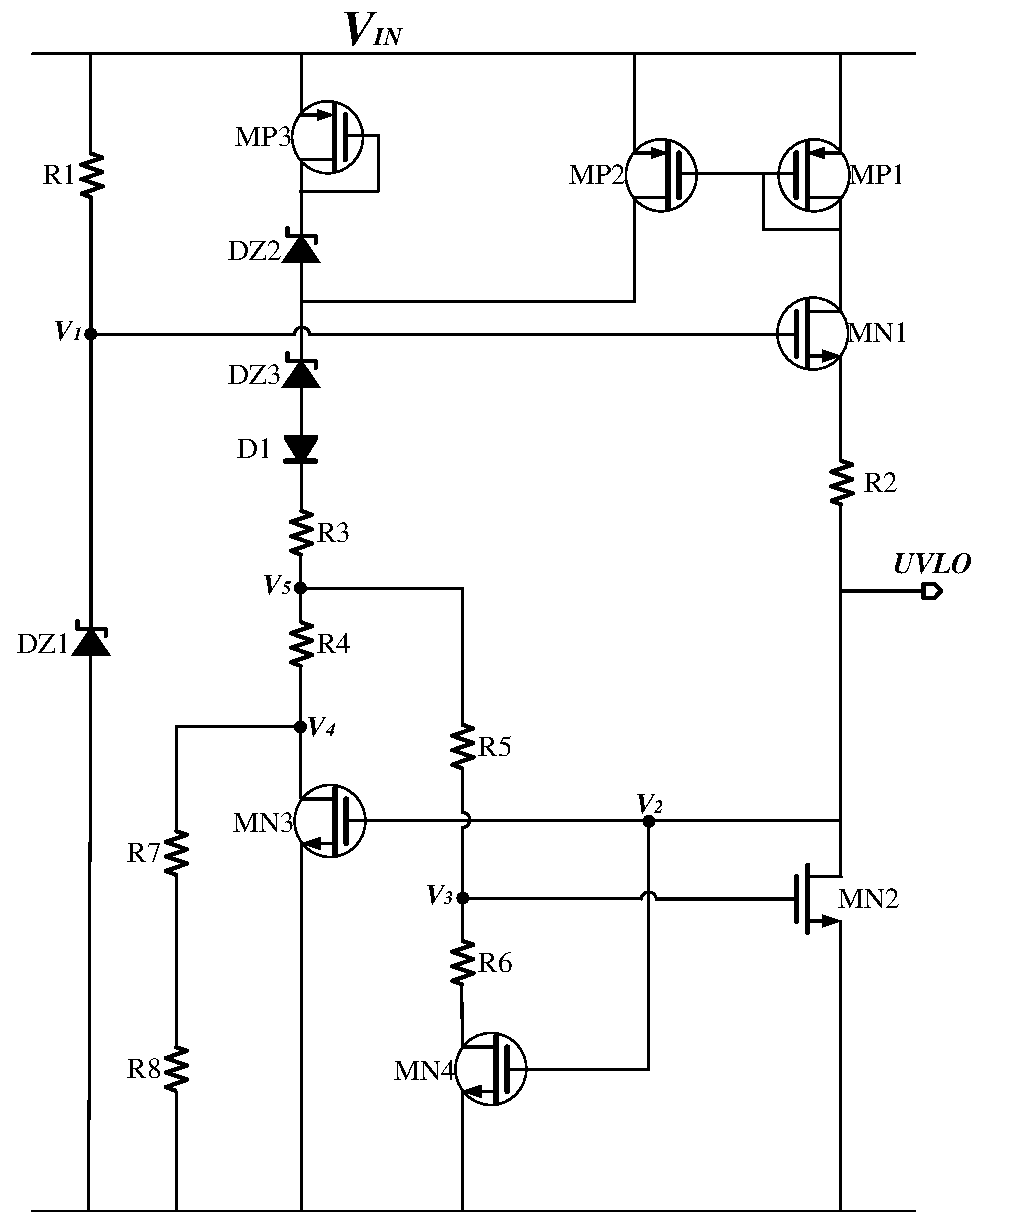
\includegraphics[width=0.6\linewidth]{figures/UVLO.pdf}
    \caption{欠压锁定UVLO电路原理图}
    \label{fig:UVLO电路}
\end{figure}

当外部输入电源电压低于预设值时,UVLO电路会输出高电平,直接控制外置功率开关管关断,同时内部低压电源供电电压均输出低电平;当外部电源电压高于预设值(即正常输入)时,UVLO输出低电平, 内部低压供电电源电压正常输出5V电压,表示芯片上电启动完成。电路原理图如图~\ref{fig:UVLO电路}所示。

欠压锁定电路的工作原理是通过高压LDMOS和齐纳二极管对输入电压进行箝位,当输入电压逐渐升高到大于齐纳二极管$D_{Z1}$时,节点电压V1被箝位至二极管$D_{Z1}$的反向击穿电压$V_{DZ1}$,V1作为高压管MN1的栅极电压同时将其导通。MN1导通后由于MN2未导通故无电流产生,其源端电压等于UVLO,此时UVLO电压较大,可视为逻辑“1”。MN3和MN4同时被栅极电压UVLO导通,将MN3和MN4的漏端同时拉到地电位,电阻R4并联于R5和R6的串联。
随着输入电压继续增大,节点电压V5由于自偏置高压管MP3产生的电流持续流过电阻R3,节点电压V6、V5和V4也随着输入电压持续增大。其中V6电压的公式为:
\begin{equation}
    %\label{eq:Vbe公式}
    V_6 = V_{IN} - V_{GS,MP3} - V_{DZ2} - V_{DZ3} - V_{D4}  
\end{equation}
直至节点电压V4增大至大于晶体管MN2的阈值电压$V_{TH,MN2}$时,晶体管MN2导通,将输出电压UVLO直接拉低到地电位,表明此刻输入电压脱离欠压锁定状态。此时的输入电压等于脱离欠压锁定的电压$V_{UVLO,OFF}$的电压值,电压$V_{UVLO,OFF}$的公式可表达为:
\begin{equation}
    \label{eq:V_UVLO,OFF公式}
    V_{UVLO,OFF} = V_5 + I_{R3}R_3 + V_{GS,MP3} + V_{DZ2} + V_{DZ3} + V_{D4}  
\end{equation}
其中R3上流过的电流$I_{R3}$的公式可表示为:
\begin{equation}
    \label{eq:IR3公式}
    I_{R3} = I_{R4} + I_{R5} = \frac{V_5 - V_{DS,MN3}}{R_4} +  \frac{V_5 - V_{GS,MN2}}{R_5}
\end{equation}

当输入电压从高压逐渐降低到一定值时,同样会进入欠压锁定情况中。在未进入欠压锁定状态时,由于MN4在输出UVLO为低电平时被关断,此时节点电压V4和V5相等。
随着输入电压逐渐降低,节点电压V4和V5的电压值也跟随着降低,直至当输入电压低于齐纳二极管的的反向击穿电压时,V5也低于晶体管MN2的阈值电压$V_{TH,MN2}$时,晶体管MN2关断,其漏端电压UVLO重新被瞬间拉高,电路再次进入欠压锁定转态。

\subsection{欠压锁定电路仿真分析}

\begin{figure}[htbp] 
    \centering
    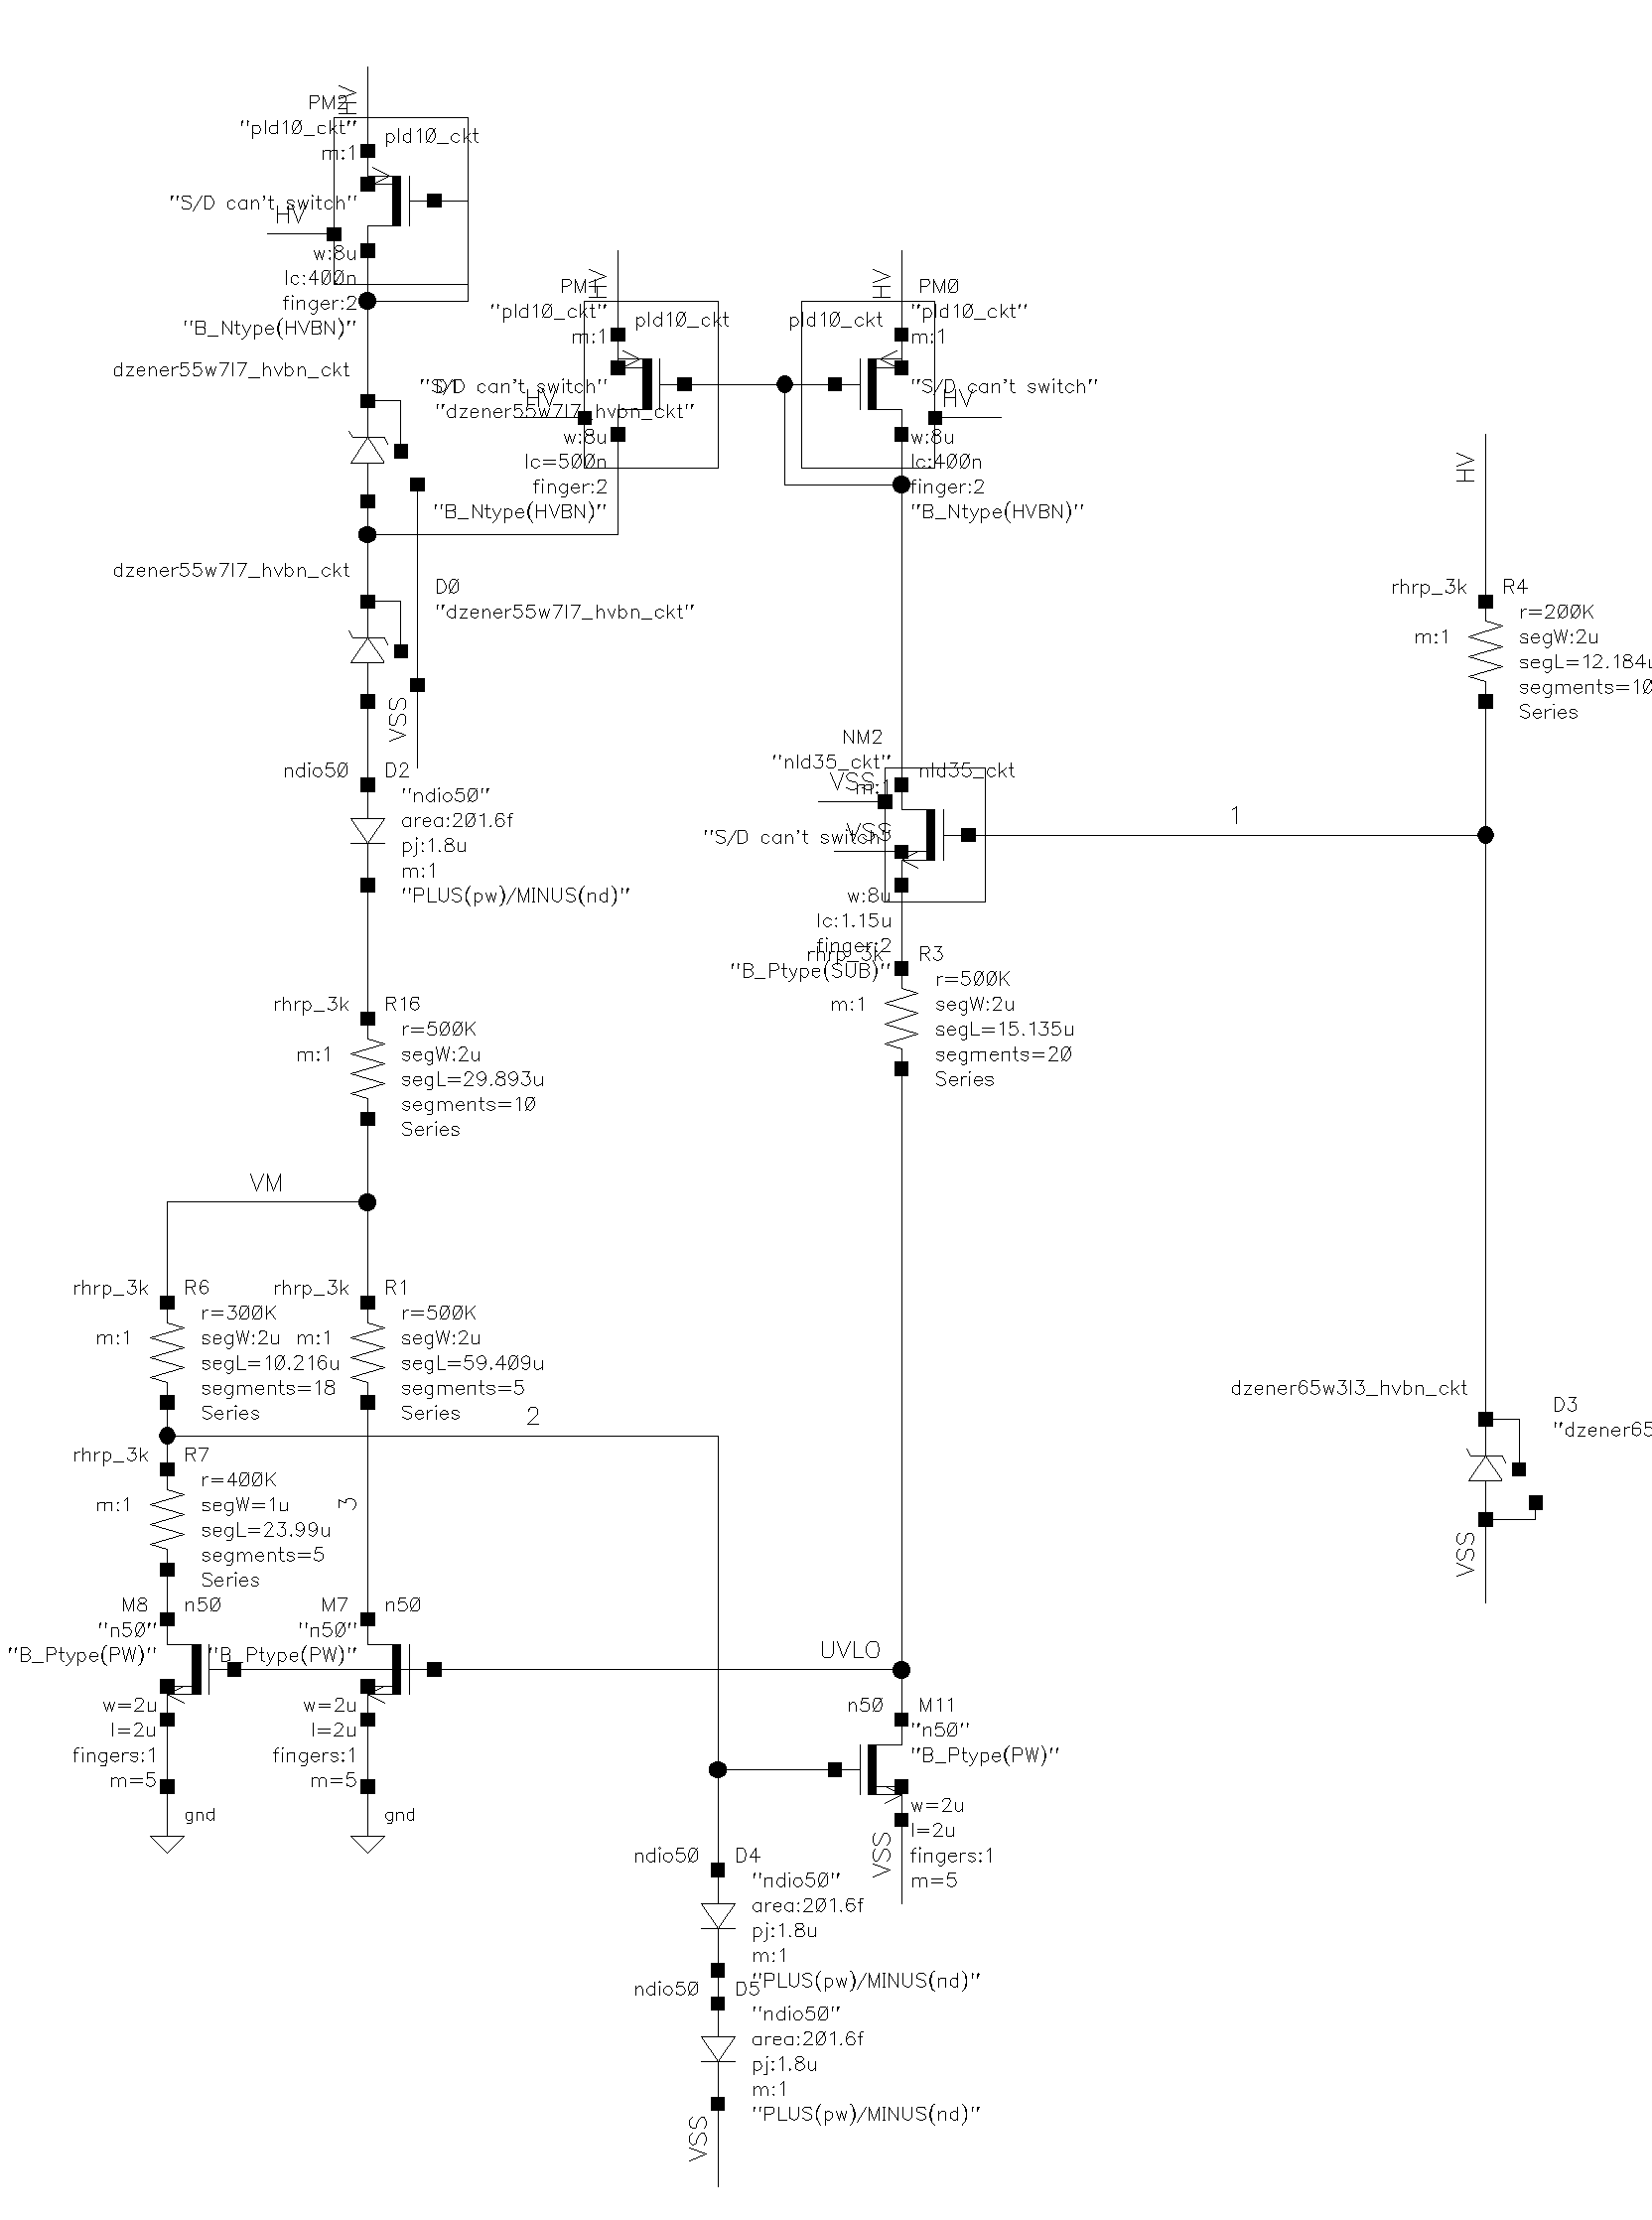
\includegraphics[width=0.8\linewidth]{figures/UVLO.png}
    \caption{欠压锁定UVLO电路仿真图}
    \label{fig:UVLO电路仿真}
\end{figure}

欠压锁定电路的仿真结果如图~\ref{fig:UVLO电路仿真}所示。
仿真结果表明,该欠压锁定电路正常完成其功能,性能符合变换器芯片要求。测试所用的输入电压HV输入范围为0-20V,当输入电压从低压逐渐升高至14.3V前,欠压锁定电路的输出电压UVLO电压为高电平,表明此时电路处于欠压锁定状态,芯片内部模块都未开始工作;当输入电压大于14.3V后,输出电压UVLO翻转为低电平,片内各模块进入正常工作转态。当输入电压从高压逐渐降低至6.5V时,欠压锁定电路输出电压UVLO重新被提升至高电平,电路重新进入欠压锁定状态,片内所有电路重新停止工作。



\iffalse
\section{内部供电电路}

\subsection{带隙基准电路}

在变换器芯片工作过程中,其内部的各个模块都需要相应的偏置电压和偏置电流,为了维持这些偏置电压和偏置电流的精确和稳定性,不能用普通的与电源无关的基准电路产生全部的信号,因此需要设计带隙基准电路,提供受电源电压和温度变化影响很小的基准电压电流,使得变换器芯片适用于各种工况下。

带隙基准电路的实现原理是通过将一个正温度系数的电压和一个负温度系数的电压加权相加后,抵消掉其正负温度系数,得到不受温度变化影响的零温度系数的基准电压。实际电路中,负温度系数的电压利用双极型晶体管产生,其正向压降$V_{be}$带有负温度特性。通过半导体物理的基础知识可知,电压$V_{be}$的公式为:
\begin{equation}
    \label{eq:Vbe公式}
    V_{be} = V_T \cdot ln(\frac{I_c}{I_s})
\end{equation}
其中,$V_T$是热电压,公式为:
\begin{equation}
    \label{eq:VT公式}
    V_T=\frac{kT}{q}
\end{equation}
$I_c$是PN结的集电极电流,公式为:
\begin{equation}
    \label{eq:Ic公式}
    I_c=I_s \cdot exp(\frac{V_{be}}{V_T})
\end{equation}
$I_s$是PN结饱和电流,公式为:
\begin{equation}
    \label{eq:Is公式}
    I_s=bT^{4+m} exp\frac{-E_g}{kT}
\end{equation}
结合式\eqref{eq:Vbe公式}、\eqref{eq:Ic公式}和\eqref{eq:Is公式},通过正向压降$V_{be}$对温度求偏导,可计算得$V_{be}$的负温度系数公式:
\begin{equation}
    \label{eq:Vbe/T公式}
    \frac{\partial V_{be}}{\partial T} = \frac{ V_{be} - (4+m)V_T - E_g/q}{T}
\end{equation}

正温度系数的电压同样可以通过双极型晶体管来产生,不同电流密度的电流流经晶体管会产生不同的负温度系数,两者的差值电压$\varDelta V_{be}$带有正温度系数。实际电路中为了满足晶体管的匹配性,使用两个不同面积的双极型晶体管来产生不同电流密度的作用。令两个双极型晶体管的面积比为$1:N$,则流经单个晶体管的电流密度比N:1,可计算得晶体管压差$\varDelta V_{be}$的公式为:
\begin{equation}
    \label{eq:△Vbe公式}
    \varDelta V_{be} = V_T ln(\frac{I_c}{I_s}) - V_T ln(\frac{I_c}{nI_s}) = V_T \cdot ln(n)
\end{equation}
通过$\varDelta V_{be}$对温度求偏导可计算得正的温度系数公式:
\begin{equation}
    \label{eq:△Vbe/T公式}
    \frac{\partial \varDelta V_{be}}{\partial T} = \frac{k}{q}\cdot ln(n)
\end{equation}


由式\eqref{eq:Vbe/T公式}和\eqref{eq:△Vbe/T公式}计算可知,在常温T=300K的条件下,当$V_{be}\thickapprox $ 750 mV时,$V_{be}$的负温度系数约等于-1.5 mV/K,$\varDelta V_{be}$的正温度系数为0.087ln(n) mV/K。为了合理地产生零温度系数电压,防止双极型晶体管的面积太大,需对正负温度系数加权相加可得。

为了满足变换器芯片中的低压数字模块,



\subsection{高压LDO电路}

由辅助绕组产生的供电端电压对于片内的元器件而已电压过大且不够稳定,无法直接用于作为供电电压,需要设计用于产生稳定输出电压的低压线性稳压器电路,将供电端的高压转化为可为内部电路供电的电源电压输出。
\begin{figure}[htbp] 
    \centering
    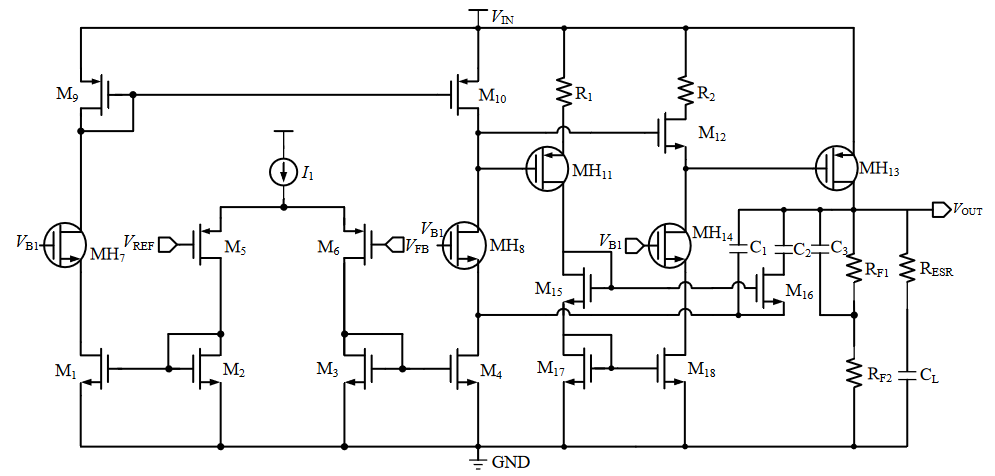
\includegraphics[width=0.6\linewidth]{figures/高压LDO.png}
    \caption{高压LDO电路图}
    \label{fig:高压LDO}
\end{figure}

本文设计的高压LDO电路如图~\ref{fig:高压LDO}所示,该电路
\fi

%\section{抖频振荡器}

%\section{模式切换电路}



\section{宽输出电压补偿的峰值电流控制电路}
\label{sec:峰值电流控制电路}
\subsection{宽输出电压补偿的峰值电流控制电路工作原理}

在宽输出范围非对称半桥反激式变换器系统中,随着输出电压的提升,相同负载下输出功率也随之提高,低输出电压下的高边功率管导通时间HSGD内存储在励磁电感和谐振腔内的能量已无法满足高输出电压下输出功率的要求,系统将自动提高峰值电流电压以产生更长的导通时间HSGD存储更多的能量传递到副边,进而要求更大的副边反馈电压$V_{FB}$,影响电路内各种模块的正常功能,产生各种不稳定的情况。

副边反馈电压$V_{FB}$随输出电压的波动是因为其是峰值电流电压$V_{CSP}$的重要组成部分,为了满足变大的输出功率,在开关频率不变的情况下,高边功率管更长的导通时间对应着更大的峰值电流$V_{CSP}$,$V_{FB}$也相应地增大。
故为满足变换器系统的宽输出范围的工作需求,设计了宽输出电压补偿结构的峰值电流控制电路来根据输出电压对峰值电流电压$V_{CSP}$进行补偿,维持副边反馈信号在宽输出范围内均匀地分布在全负载下。

%根据上文~\ref{sec:电流控制模式}小节的分析,如图~\ref{fig:电流工作模式电路图}中所示,可知副边反馈引脚电压信号是峰值电流电压$V_{CSP}$的重要组成部分,其可以一定程度地反映输出负载电流的大小。当负载电流突然增大时,为了满足变大的输出功率,变压器原边需要增加高边功率管的导通时间提供更多的能量传递给输出电容,因此$V_{CSP}$增大,$V_{FB}$也相应地增大;当负载电流突然减小时,同理$V_{FB}$也相应地减小。但在不同输出电压的情况下,相同负载电流下,信号$V_{FB}$稳定后电压值却大不相同,严重影响了芯片内多种电路模块,如精确谷底导通、谷值锁定、退磁时间动态校准等模块对$V_{FB}$的采样要求。为了避免此问题,需要设计峰值电流控制电路实现在当输出电压不同时,仍能维持信号$V_{FB}$的电压值在负载电流不变情况下的一致性。

在峰值电流控制模式中,峰值电流电压$V_{CSP}$是通过采样电阻对电感电流采样实现的,具体的转换关系可表示为:
\begin{align}
    \label{eq:VCSP公式}
    V_{CSP} = I_P \cdot R_{CS} 
\end{align}
其中$I_P$为原边电感电流的峰值。

\begin{figure}[htbp] 
    \centering
    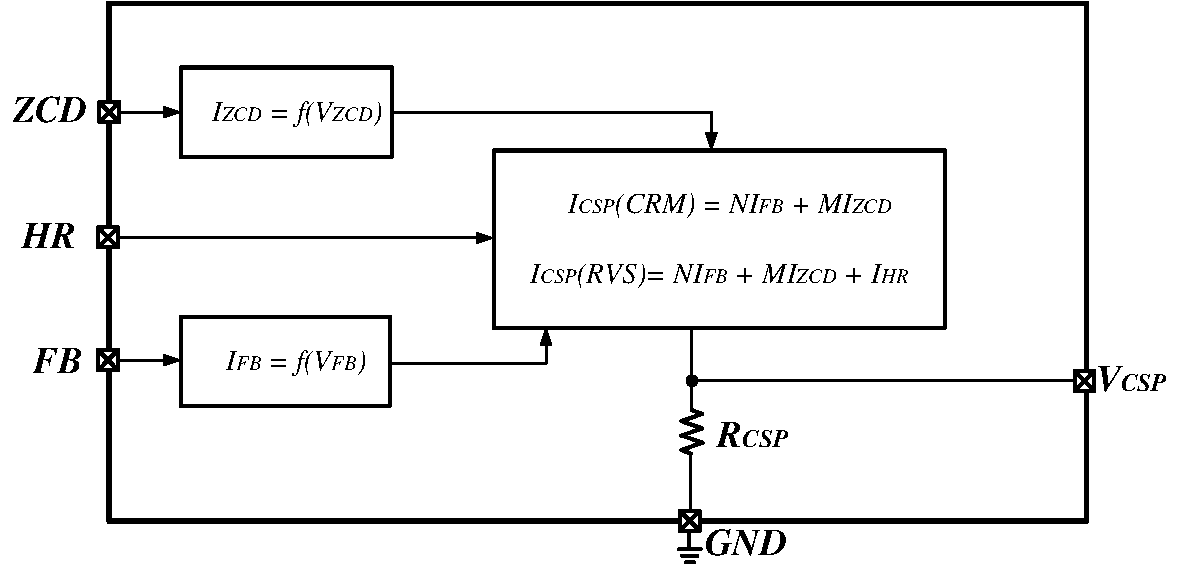
\includegraphics[width=0.8\linewidth]{figures/峰值电流控制.pdf}
    \caption{峰值电流控制电路框图}
    \label{fig:峰值电流控制框图}
\end{figure}

由于需要考虑到不同输出电压的影响,因此峰值电流电压$V_{CSP}$不能完全由副边反馈电压$V_{FB}$计算产生,需要引入携带输出电压信息的$V_{ZCD}$信号对$V_{CSP}$进行补偿,实现高边功率管导通时间在$V_{FB}$维持不变的情况下随着输出电压的变化而自动变化。其中辅助绕组电压$V_{ZCD}$和输出电压的关系如式\eqref{eq:VZCD公式}所示。

片内峰值电流电压$V_{CSP}$产生电路的框图如图~\ref{fig:峰值电流控制框图}所示,峰值电流电压$V_{CSP}$由电压信号$V_{EA}$、$V_{OVC}$和$V_{HR}$加权求和所得。电压$V_{EA}$是信号$V_{FB}$乘以反馈电压衰减系数$k_1$所得;$V_{OVC}$是输出电压补偿信号,由输出电压$V_o$乘以输出电压补偿结构衰减系数$k_2$所得;$V_{HR}$是切换为RVS工作模式时的补偿电压,用来补偿模式切换时开关频率骤变后的峰值电流变化。$V_{CSP}$的公式可表达为:
\begin{align}
    \label{eq:VCSP公式1}
    V_{CSP} &= V_{EA} + V_{OVC} + V_{HR} \\ &= k_1 V_{FB} + k_2 V_o + V_{HR}  
\end{align}
通过合理设置系数$k_1$和$k_2$的值,当输出电压切换导致$V_{CSP}$波动时,可以维持$V_{FB}$的稳定。

下面分析峰值电流电压和高边功率管导通时间在CRM工作模式中不同输出电压下的关系。图~\ref{fig:峰值电流控制1}中显示了在不同输出电压下峰值电流电压、电感电流斜率和占空比的关系。当输出电压为$V_{o1}$时,对应的峰值电流电压为$V_{CSP1}$,高边功率管导通时间HSGD为$D_1T_s$;当输出电压为$V_{o1}$时,对应的峰值电流电压为$V_{CSP2}$,高边功率管导通时间HSGD为$D_2T_s$。其中,根据式\eqref{eq:CCM_4}可求得$\frac{D2}{D1} = 4$。但由于电感电流的斜率也会发生变化,不能直接将占空比的变化值直接套用于计算$V_{CSP2}$和$V_{CSP1}$的比值。结合式\eqref{eq:Vcr_1}电感电流的斜率$K_{slope}$的公式可表示为:
\begin{equation}
    \label{eq:电感电流斜率公式}
    K_{slope} = \frac{V_{in} - N V_o}{L_m}
\end{equation}
由式\eqref{eq:电感电流斜率公式}可见,电感电流斜率会随着输出电压的变化而变化,输出电压越大,斜率越小。因此,在输出电压变化的情况下,峰值电流电压$V_{CSP}$的变化和占空比D的变化不成正比,不能直接对$V_{CSP}$乘以输出电压变化的倍数计算变化后的$V_{CSP}$。

\begin{figure}[htbp] 
    \centering
    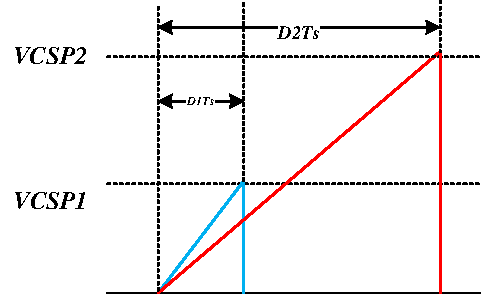
\includegraphics[width=0.6\linewidth]{figures/峰值电流控制1.pdf}
    \caption{不同输出电压下的峰值电流电压波形}
    \label{fig:峰值电流控制1}
\end{figure}

结合图~\ref{fig:峰值电流控制1}中带入公式\eqref{eq:电感电流斜率公式}得峰值电流电压的公式为:
\begin{equation}
    \label{eq:VCSP公式2}
     V_{CSP} = K_{slope} \cdot DT_s = \frac{V_{in} - N V_o}{L_m} \cdot \frac{N V_o}{V_{in}} T_s
\end{equation}

分别将两个不同的输出电压$V_{o1}$和$V_{o2}$带入式中,可计算得$V_{CSP1}$和$V_{CSP2}$的比值为:
\begin{equation}
    \label{eq:VCSP公式3}
    \frac{V_{CSP2}}{V_{CSP1}} = \frac{4 (V_{in} - NV_{o1})}{V_{in} - NV_{o2}}
\end{equation}
故当测得单一输出电压下的峰值电流电压值后,其他输出电压下的$V_{CSP}$也都可计算求出。

为计算输出电压补偿衰减系数$k_2$的值,将不同的输出电压带入式\eqref{eq:VCSP公式1}中并作差可得:
\begin{equation}
    \label{eq:VCSP公式4}
    \varDelta V_{CSP} = V_{CSP2}-V_{CSP1} = k_2 (V_{o2} - V_{o1})
\end{equation}

将式\eqref{eq:VCSP公式3}带入式\eqref{eq:VCSP公式4}中可求得输出电压补偿衰减系数$k_2$的公式为:
\begin{equation}
    \label{eq:k2公式}
    k_2 = \{ \frac{4 (V_{in} - NV_{o1})}{V_{in} - NV_{o2}} - 1 \} V_{CSP1} \cdot \frac{1}{V_{o2} - V_{o1}}
\end{equation}

\begin{figure}[htbp] 
    \centering
    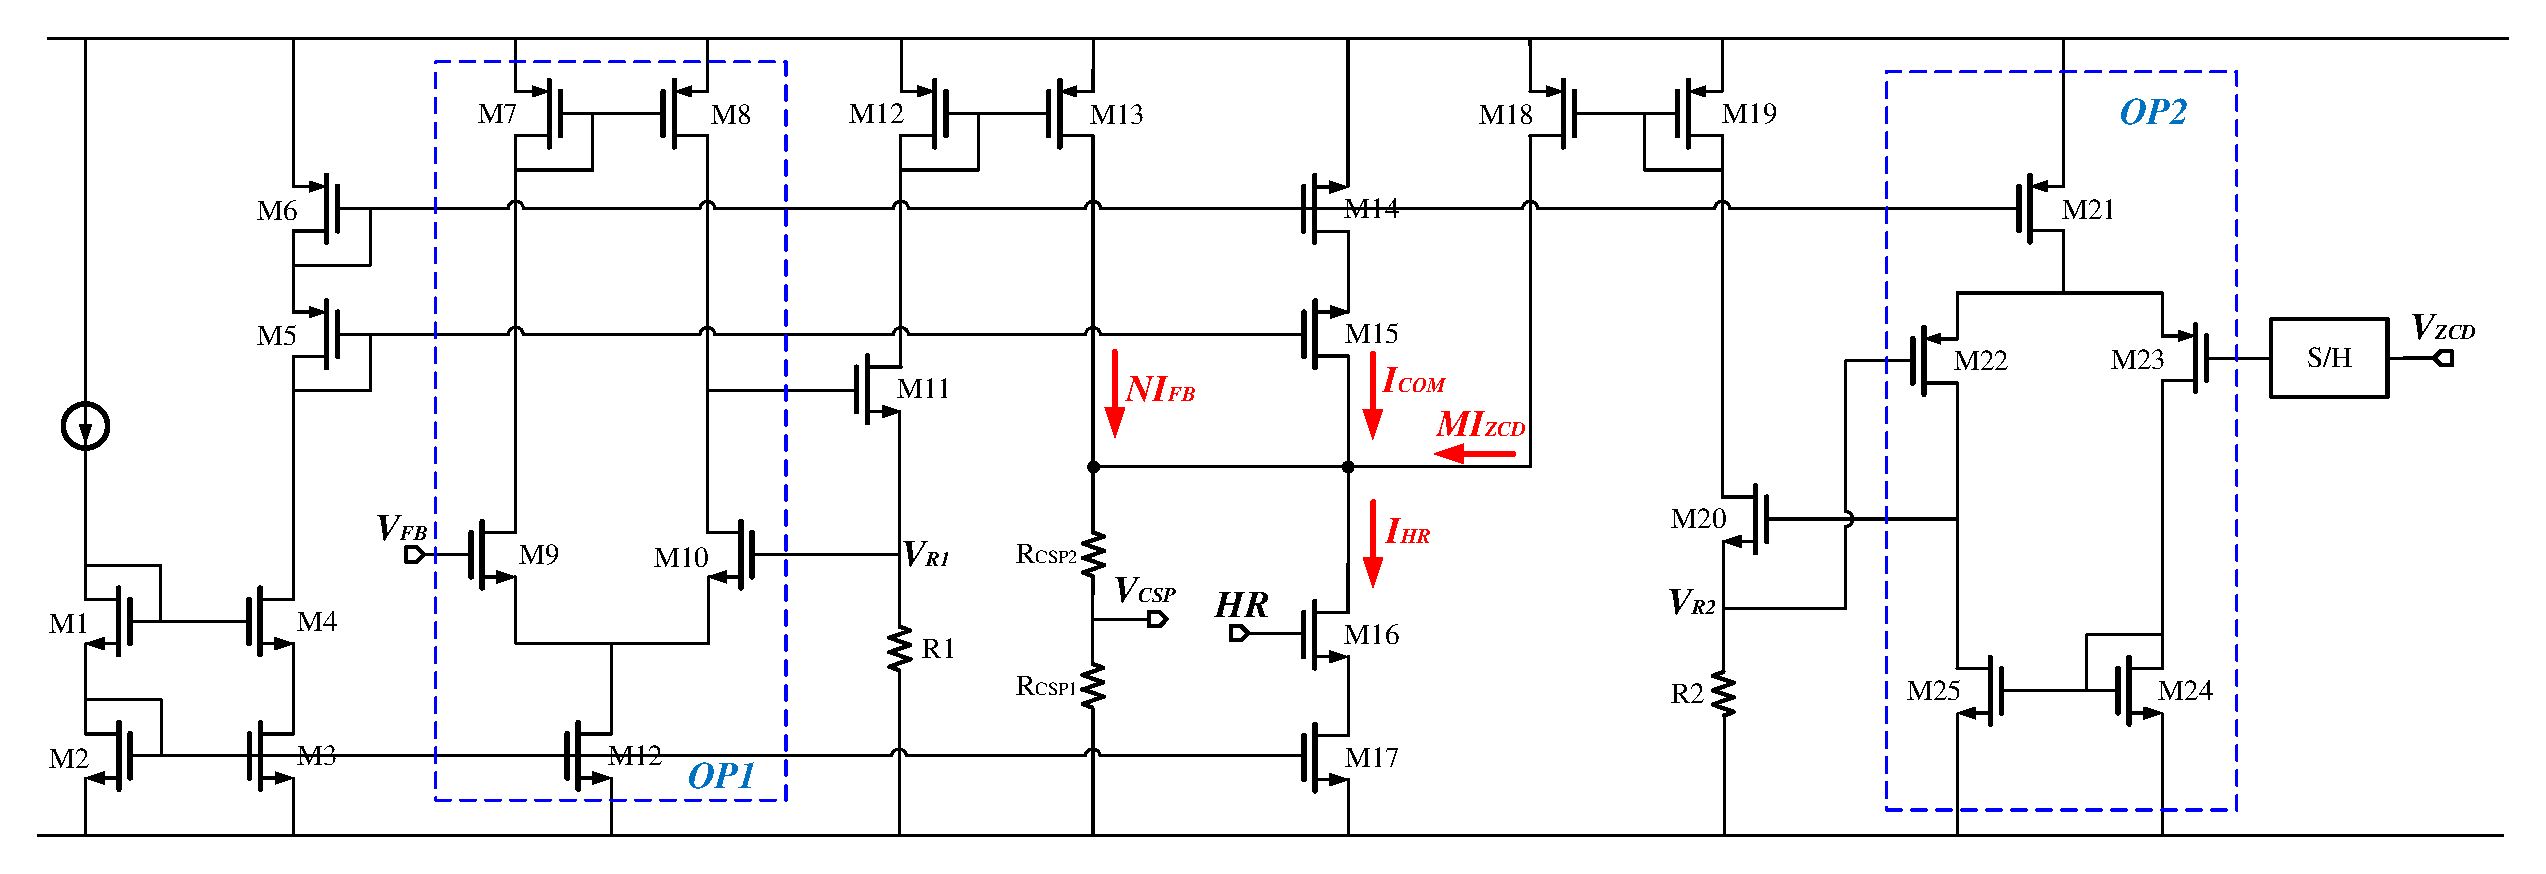
\includegraphics[width=1.0\linewidth]{figures/峰值控制电路图.pdf}
    \caption{峰值控制电路电路图}
    \label{fig:峰值控制电路图}
\end{figure}

带有宽输出电压补偿结构的峰值电流控制电路的具体电路图如图~\ref{fig:峰值控制电路图}所示。图中包括两个运放OP1和OP2组成的VCCS结构,该电路通过运放的虚短作用将OP1的输入端$V_{FB}$箝位到$V_{R1}$,$V_{R1}=V_{FB}$,调节运放输出端的电压控制晶体管M11的漏电流等于$I_{FB}$,同理运放OP2也将$V_{ZCD}$转化为电流$I_{ZCD}$。其中$I_{FB}$和$I_{ZCD}$的公式表达为:
\begin{equation}
    \label{eq:IFB公式}
    I_{FB} = \frac{V_{FB}}{R_1}
\end{equation}
\begin{equation}
    \label{eq:IZCD公式}
    V_{CSP} = \frac{V_{ZCD,in}}{R_2}
\end{equation}
电流信号$I_{FB}$通过电流镜M12、M13镜像为电流$NI_{FB}$后,该电流流过电阻$R_{CSP1}$,形成电压$V_{EA}$,其中$V_{EA}=k_1V_{FB}$;电流信号$I_{ZCD}$通过电流镜M18、M19镜像为电流$MI_{ZCD}$后,该电流同样流过电阻$R_{CSP1}$,形成电压$V_{OVC}$,$V_{OVC}$的公式可表示为:
\begin{equation}
    \label{eq:VOVC公式}
    V_{OVC} = \frac{MR_{CSP1}}{R_2}  V_{ZCD,in}
\end{equation}
除此之外,$R_{CSP1}$上的电流还包括补偿电流信号$I_{com}$和用于补偿模式切换的电流信号$I_{HR}$,分别在$R_{CSP1}$上形成电压$V_{com}$和$V_{HR}$。电压$V_{com}$用于对副边反馈电压的值进行微调,以匹配其他电路模块的工作要求。电阻$R_{CSP2}$的取值需要考虑到当工作模式切换为CRM模式时晶体管M17的过驱动电压,保证M17可以正常工作。

电路中电阻$R_1$和$R_2$的取值与对应的衰减系数$k_1$和$k_2$以及电流镜的复制比有关。当电阻$R_{CSP1}$的阻值确定后,根据反馈电压衰减系数$k_1$的值可求得电阻$R_1$为:
\begin{equation}
    \label{eq:R1公式}
    R_1 = \frac{NR_{CSP1}}{k_1}
\end{equation}
电阻$R_2$的计算公式需将公式\eqref{eq:VZCD公式}和\eqref{eq:k2公式}带入公式\eqref{eq:VOVC公式}中即可求得:
\begin{align}
    \label{eq:R2公式}
    R_2 &= \frac{MR_{CSP1}}{V_{OVC}}  V_{ZCD} = \frac{R_{CSP1}}{k_2 V_o}  V_{ZCD}
    \\  &= \frac{MR_{CSP1}}{\{ \frac{4 (V_{in} - NV_{o1})}{V_{in} - NV_{o2}} - 1 \} V_{CSP1} \cdot \frac{1}{V_{o2} - V_{o1}}}  \frac{N_A}{N_S}\frac{R_{a2}}{R_{a1}+R_{a2}}
\end{align}


\subsection{宽输出电压补偿的峰值电流控制电路仿真分析}




%\section{前沿消隐电路}



\section{精确谷底导通电路}

\subsection{精确谷底导通电路原理}

根据上文3.6.2节介绍的精确谷底导通技术,本小节对图~\ref{fig:精确谷底导通技术框图}中的精确谷底导通模块进行具体的描述并仿真其基本功能。

图~\ref{fig:精确谷底导通电路图1}是精确谷底导通模块的电路框图。包括两个峰值检测电路、压控高通滤波器、SR锁存器、鉴相鉴频器、电荷泵和逻辑电路等。

\begin{figure}[htbp] 
    \centering
    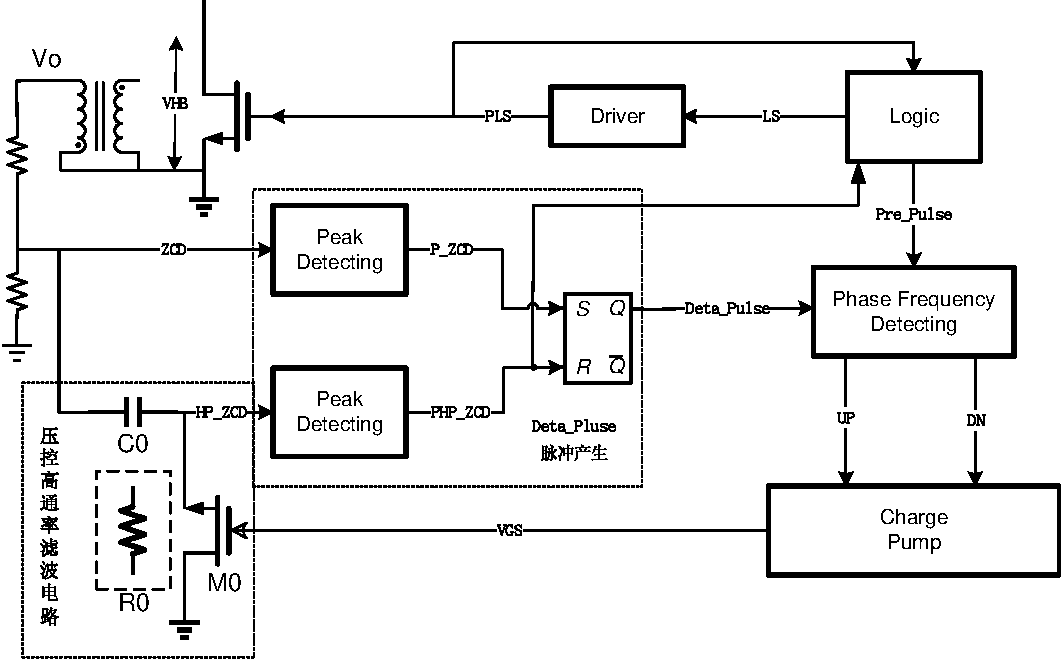
\includegraphics[width=0.8\linewidth]{figures/精确谷底导通电路图1.pdf}
    \caption{精确谷底导通电路图1}
    \label{fig:精确谷底导通电路图1}
\end{figure}


因为功率管半桥节点信号$V_{HB}$的电压值过大,无法直接输入变换器芯片内进行处理,因此对在等待时间$T_w$内同样带有谐振信息的辅助绕组分压引脚ZCD的电压信号$V_{ZCD}$进行采样处理。由于$V_{ZCD}$信号和$V_{HB}$信号的谐振电压相位相反,故$V_{HB}$的谐振谷底对应$V_{ZCD}$的谐振谷峰值。如图~\ref{fig:精确谷底导通电路图1}中所示,采用峰值检测电路来检测$V_{ZCD}$信号在等待时间$T_w$内的谐振谷峰值,并输出对应的峰值脉冲信号P\_ZCD。

峰值检测电路图如图~\ref{fig:峰值检测电路图}所示。峰值检测电路包括一个由晶体管M2、M4、M5、M6和M7组成的五管运算放大器,一个晶体管M9和M10组成的电流镜以及晶体管M11构成的源极跟随器。电流镜晶体管M12为源极跟随器M11提供偏置电流。该电路的工作原理是通过运算放大器比较输入电压$V_{in}$和输出电压$V_{out}$的大小,当输入电压$V_{in}$大于输出电压$V_{out}$时,运算放大器输出低电平,拉低电流镜晶体管M9的栅端电压,电流镜开始工作,对电容$C_1$进行充电,电压$V_1$逐渐升高,$V_{out}$在源极跟随器的作用下也逐渐增大,跟随$V_{in}$变化。当$V_{in}$不再增大,$V_{in}$开始小于$V_{out}$时,运算放大器输出高电平,拉高电流镜晶体管M9的栅端电压,电流镜停止工作,不再给电容$C_1$进行充电,进而输出电压$V_{out}$也保持不变,实现峰值检测的功能。最后通过一个脉冲产生电路输出峰值脉冲信号。同时为了检测在电路在不同周期内不同大小的输入电压$V_{in}$,加入复位开关管M13,当接收到复位信号$R_{st}$后,开关管M13导通,对电容$C_1$进行放电,实现复位的功能。

\begin{figure}[htbp] 
    \centering
    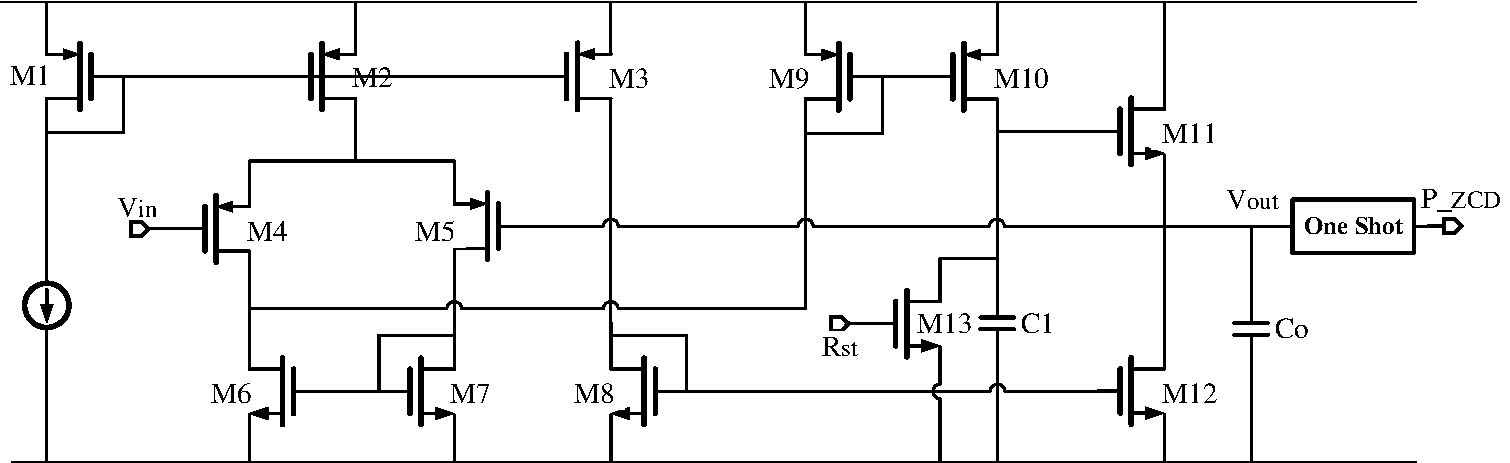
\includegraphics[width=1.0\linewidth]{figures/峰值检测电路图.pdf}
    \caption{峰值检测电路图}
    \label{fig:峰值检测电路图}
\end{figure}

由于驱动电路等电路结构对逻辑控制信号存在延时问题,为了满足精确的谷底导通功能,不能直接将信号$V_{ZCD}$通过峰值检测电路产生的峰值脉冲信号P\_ZCD直接作为时钟信号CLK输入到逻辑控制模块来产生下个开关周期的逻辑控制信号LS。针对于该问题,新颖性地提出了迫使精确谷底导通模块在$V_{HB}$谐振谷底到达之前产生低边功率管的导通时钟信号CLK的方案,使得逻辑控制信号LS通过驱动电路延时后,输出的栅极驱动信号LSGD恰好位于$V_{HB}$信号谐振谷底的位置处,此时导通低边功率管,不仅降低开关损耗,还可以极大地减小峰值检测电压的过冲现象。为满足该功能,要求逻辑控制信号LS超前产生的时间近似等于驱动电路等结构的延时时间。

该模块中实现超前采样$V_{ZCD}$信号峰值的核心电路是采用的压控高通滤波器电路,如图~\ref{fig:精确谷底导通电路图1}中所示,可以通过控制MOS管的栅极电压$V_{GS}$来调节MOS管的导通电阻$R_{on}$,$R_{on}$的计算公式为:
\begin{equation}
    \label{eq:Ron公式}
    R_{on}=\frac{1}{\mu_n C_{ox} \frac{W}{L} (V_{GS} - V_{TH})}
\end{equation}
由式可知,随着MOS管栅极电压$V_{GS}$的增大,其导通电阻逐渐减小。根据高通滤波器的幅频曲线公式可知,当功率管栅压$V_{GS}$为零电压时,功率管截止,导通电阻近似无穷大,对应的时间常数RC无穷大,相位变化为0度,压控高通滤波器的输出信号$V_{ZCD,PH}$和信号$V_{ZCD}$的电压波形重合。随着栅压信号$V_{GS}$的增大,时间RC常数越小,$V_{ZCD,PH}$波形超前的相位变化越大,直至时间常数RC等于零时,超前相位最大值90度。
\begin{equation}
    \label{eq:jw公式}
    \varphi_{j\omega }=\arctan (\frac{\omega_c}{j\omega R C })
\end{equation}
其中$\omega_c$为滤波器的截止频率。通过和合理的调节MOS管栅压信号$V_{GS}$的值,即可调节$V_{ZCD,ph}$波形恰好超前$V_{ZCD}$电压波形的相位时间信号D\_Phase和驱动电路的延时时间信号L\_Phase的脉冲宽度相等,实现低边功率管栅极驱动信号的精确谷底导通功能。其中,如图~\ref{fig:精确谷底导通电路图1},信号D\_Phase是信号$V_{ZCD,PH}$和$V_{ZCD}$通过峰值采样电路分别输出的峰值脉冲信号PH\_ZCD与P\_ZCD经过一个SR锁存器产生的;信号L\_Phase则是将栅极驱动信号LSGD经过电平移位器降为低压后同逻辑控制信号LS经过SR锁存器产生的。

\begin{figure}[htbp] 
    \centering
    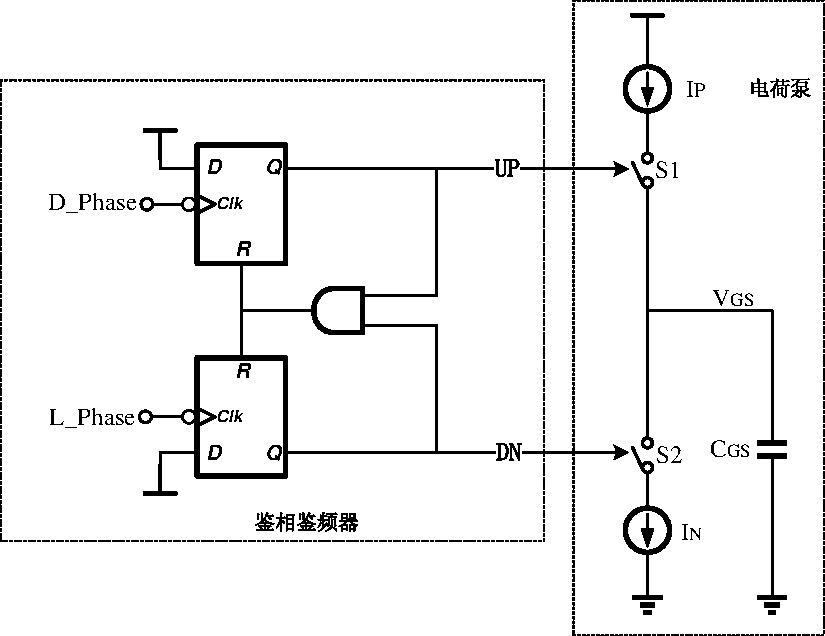
\includegraphics[width=0.8\linewidth]{figures/鉴相鉴频器.pdf}
    \caption{鉴相鉴频器和电荷泵电路图}
    \label{fig:鉴相鉴频器电路图}
\end{figure}

压控高通滤波器的栅压信号$V_{GS}$的调控方式采用了锁相环电路中的鉴相鉴频器和电荷泵结构来动态调节实现。图~\ref{fig:鉴相鉴频器电路图}为该模块使用的鉴相鉴频器电路和电荷泵的电路图。包括两个带复位端的下降沿D触发器和一个与门组成。触发器的D输入端都接高电平保持逻辑"1",触发器1的时钟输入端D\_Phase是信号$V_{ZCD,PH}$和信号$V_{ZCD}$波形的超前相位时间差;触发器2的时钟输入端L\_Phase是逻辑控制信号LS和栅压驱动信号LSGD的延迟时间差。通过这两个D触发器检测D\_Phase和L\_Phase信号的相位时间差信号UP和DN,再通过信号UP和DN控制电荷泵的开关S1和S2,选择对电容$C_{GS}$进行充电或放电功能。


鉴相鉴频器和电荷的波形图如~\ref{fig:鉴相鉴频器波形图}所示。不同于上升沿D触发器组成的鉴相鉴频器,该模块中使用的下降沿鉴相鉴频器的输出信号UP和DN是信号D\_Phase和L\_Phase的下降沿的相位时间差。当信号D\_Phase先于信号L\_Phase变为低电平时,信号UP由低变高,导通开关S1,电流源$I_P$对电容$C_{GS}$进行充电,电压$V_{GS}$逐渐增大;当信号L\_Phase的下降沿到来后,UP由高变低,开关S1关断,$V_{GS}$保持不变。同理,信号DN和UP相似,区别在于L\_Phase先于信号D\_Phase变为低电平时有低变高,导通开关S2通过电流源$I_N$对电容$C_{GS}$进行放电,电压$V_{GS}$逐渐减小。随着鉴相鉴频器和电荷泵电路的不断工作,最终信号D\_Phase和信号L\_Phase几乎重叠,信号UP和DN脉冲保持一致,同时给电容$C_{GS}$进行充电和放电,电压$V_{GS}$维持稳定。

\begin{figure}[htbp] 
    \centering
    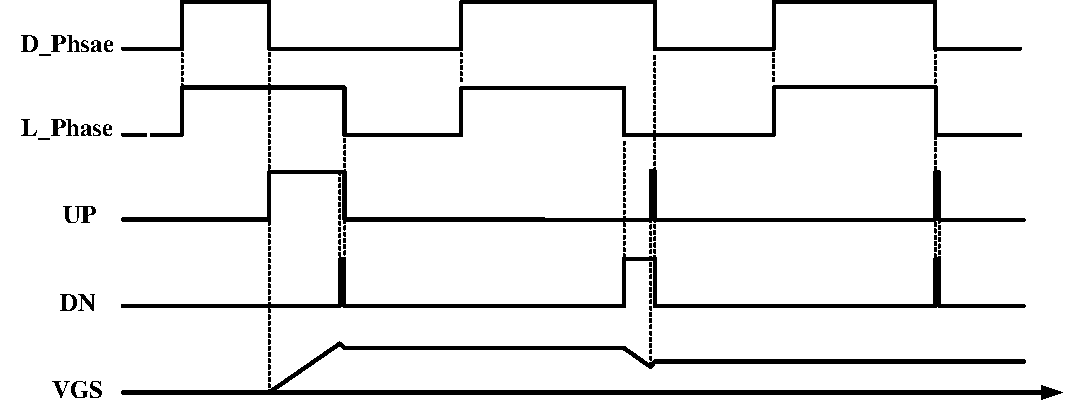
\includegraphics[width=0.8\linewidth]{figures/鉴相鉴频器波形图.pdf}
    \caption{鉴相鉴频器电荷泵波形图}
    \label{fig:鉴相鉴频器波形图}
\end{figure} 

其中,模块中使用的单端结构电荷泵的实际电路图如图~\ref{fig:电荷泵电路图}所示,电荷泵的单端结构占用面积较小,且更易于设计,满足于精确谷底导通模块的使用需求。同时为了减小电荷泵电路中的电荷注入、时钟馈通和电荷共享的非理性效应,采用了源极开关型结构。该电荷泵结构未直接将MOS开关管MP5、MN4连接在电容$C_{GS}$的上极板,通过电流镜晶体管MP6、MN3将开光管和电容隔离开,阻挡了开关管关断时反型层中的沟道电荷注入电容,提高了电压$V_{GS}$的稳定性。

\begin{figure}[htbp] 
    \centering
    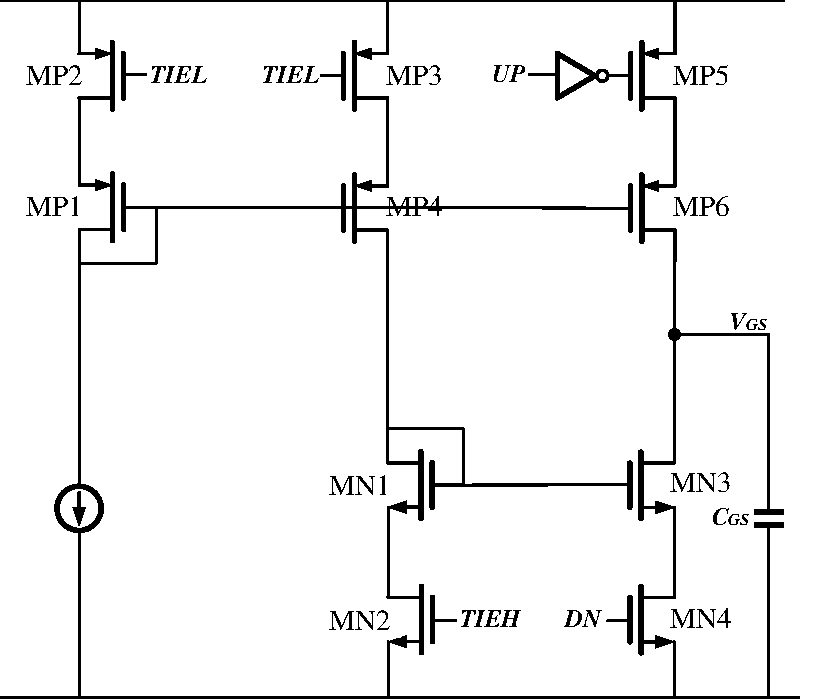
\includegraphics[width=0.7\linewidth]{figures/电荷泵电路图.pdf}
    \caption{电荷泵电路图}
    \label{fig:电荷泵电路图}
\end{figure} 

为了满足PMOS管在信号UP的控制下正确地导通和关断,通过一个反相器输出信号UPN来控制开关管MP5,在信号UP电压由低变高时,信号UPN电压由高变低,导通开关管MP5,对电容$C_{GS}$进行充电;信号DN电压由低变高时,直接控制开关管MN4导通,对电容$C_{GS}$进行放电。电荷泵电路除了由晶体管MP1、MP4、MP6组成的PMOS电流镜和晶体管MN1、MN3组成的NMOS电流镜,还额外加入了晶体管MP2、MP3、MN2来和开关管MP5 MN4相对应,提高了电路的对称性,在开关管导通时使得电流镜晶体管的源极电压相等,提高电流镜的复制比精度,迫使电容$C_{GS}$的充放电电流尽可能一致。


结合图~\ref{fig:精确谷底导通波形图}中的工作波形,精确谷底导通模块的具体工作过程为:当工作模式首次切换为RVS模式时,此时压控高通滤波器的栅压$V_{GS}$为零,晶体管M0未导通,晶体管的导通电阻近似无穷大,高通滤波器的相位变化为零,信号$V_{ZCD,PH}$和信号$V_{ZCD}$波形重叠,模块将峰值检测电路检测的$V_{ZCD}$峰值脉冲信号P\_ZCD作为时钟CLK输出给逻辑控制模块,产生的逻辑控制信号LS在t1时刻的$V_{HB}$谐振谷底处由低电平变为高电平,经过驱动电路延时后,栅极驱动信号在t2时刻控制低边功率管导通,此时$V_{HB}$电压较大,产生较大的开关损耗。信号D\_Phase和L\_Phase经过鉴相鉴频器输出的信号UP导通电荷泵开关管对电容充电,压控高通滤波器栅压$V_{GS}$线性增大。

\begin{figure}[htbp] 
    \centering
    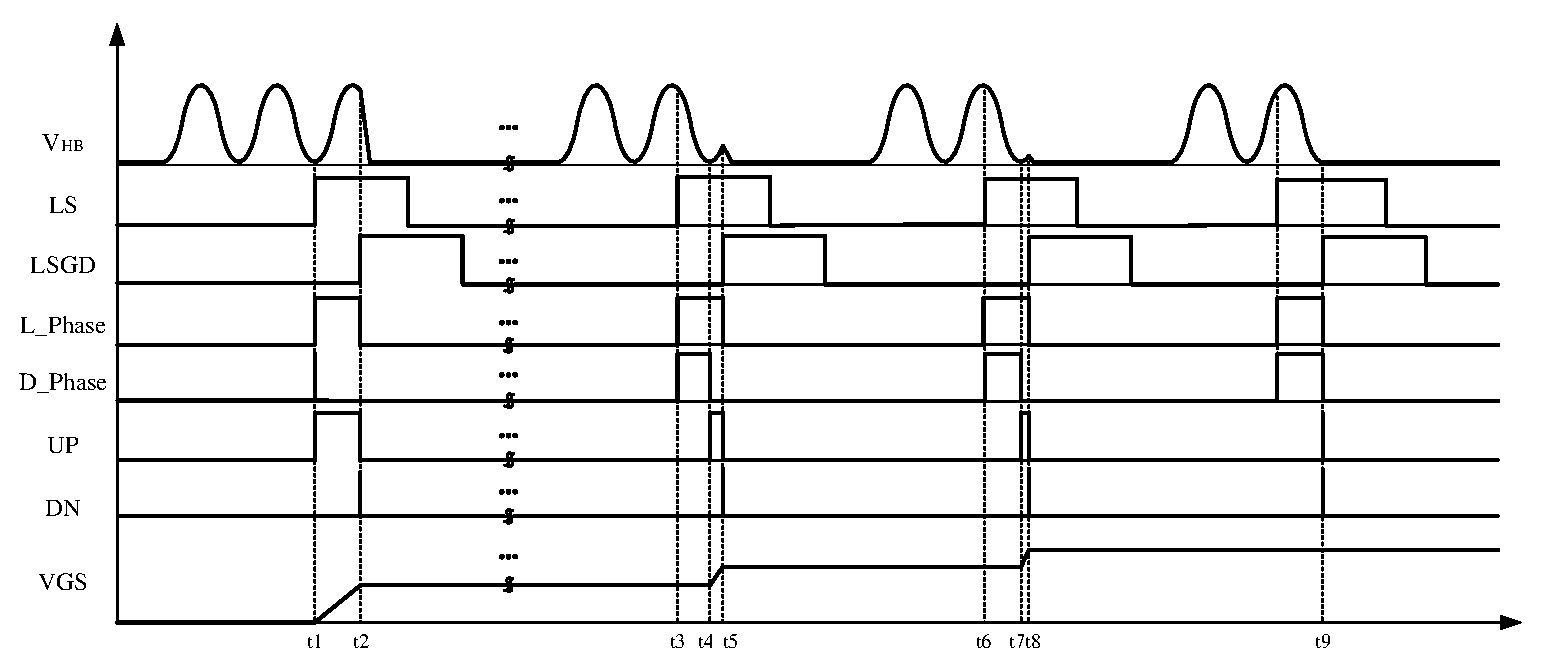
\includegraphics[width=1.0\linewidth]{figures/精确谷底导通波形图.pdf}
    \caption{精确谷底导通电路相关波形图}
    \label{fig:精确谷底导通波形图}
\end{figure} 

经过几个开关周期的充电后,栅压$V_{GS}$大于晶体管M0阈值电压,晶体管导通,压控高通滤波器产生的超前信号D\_Phase迫使信号LS在$V_{HB}$谐振谷底前导通,与信号L\_Phase之间的相位差UP也相应减小,成功实现逐步逼近功能,栅极驱动信号LSGD在t5时刻导通低边功率管,此时虽仍未在谷底处导通,但开关损耗已大大降低。

最后经过几个开关周期的变化,压控高通滤波器产生的超前信号D\_Phase几乎与信号L\_Phase重叠,鉴相鉴频器输出信号UP和DN脉冲宽度相等,电容上电压$V_{GS}$维持稳定,t9时刻LSGD在$V_{HB}$谐振谷底处实现精确导通低边功率管的功能。

\subsection{精确谷底导通电路仿真分析}


图~\ref{fig:谷底导通仿真图}为精确谷底导通电路相关波形仿真图,由仿真图可见,当系统由恒流模式切换为恒压模式中的RVS工作模式后,精确谷底导通模块内压控高通滤波器的栅压$V_{GS}$随着开关周期逐渐增大,经过1.43ms后稳定在1.65V,此时电路已完成精确谷底导通功能。图~\ref{fig:谷底导通放大仿真图}中分别展示了电路在栅压$V_{GS}$未稳定和稳定后的具体波形图。在图~\ref{fig:谷底导通放大仿真图} (a)中,栅极驱动信号LSGD未能在$V_{HB}$谐振谷底处导通,其导通时刻$V_{HB}$电压值等于27.7V,和谷底处电压值的差值约为21.3V。在图~\ref{fig:谷底导通放大仿真图} (b)中可见,由于电路精度的限制,栅极驱动信号LSGD导通低边功率管时$V_{HB}$电压值和谷底电压值的差值仅为252mV,可以近似忽略不计,实现了电路的设计需求和功能。

%通过逻辑控制电路得到LS和PLS信号的延时时间Pre\_Pulse。为了预判谷底信号,通过一个使用MOS管充当电阻的压控高通滤波器电路,产生$V_{ZCD}$对应的超前时间信号VHP\_ZCD,只需适当的调节VGS的大小即可控制VHP\_ZCD信号的超前时间大小。分别使用两个峰值检测电路来检测并得到两个信号的峰值脉冲信号,经过SR锁存器产生超前时间Deta\_Pulse。为了轻微的调节栅极电压信号VGS,使用了PLL电路中的鉴相鉴频器和电荷泵电路来控制Deta\_Pulse信号逐步逼近Pre\_Pulse信号,完成低边功率管的精确谷底导通功能。

\begin{figure}[htbp] 
    \centering
    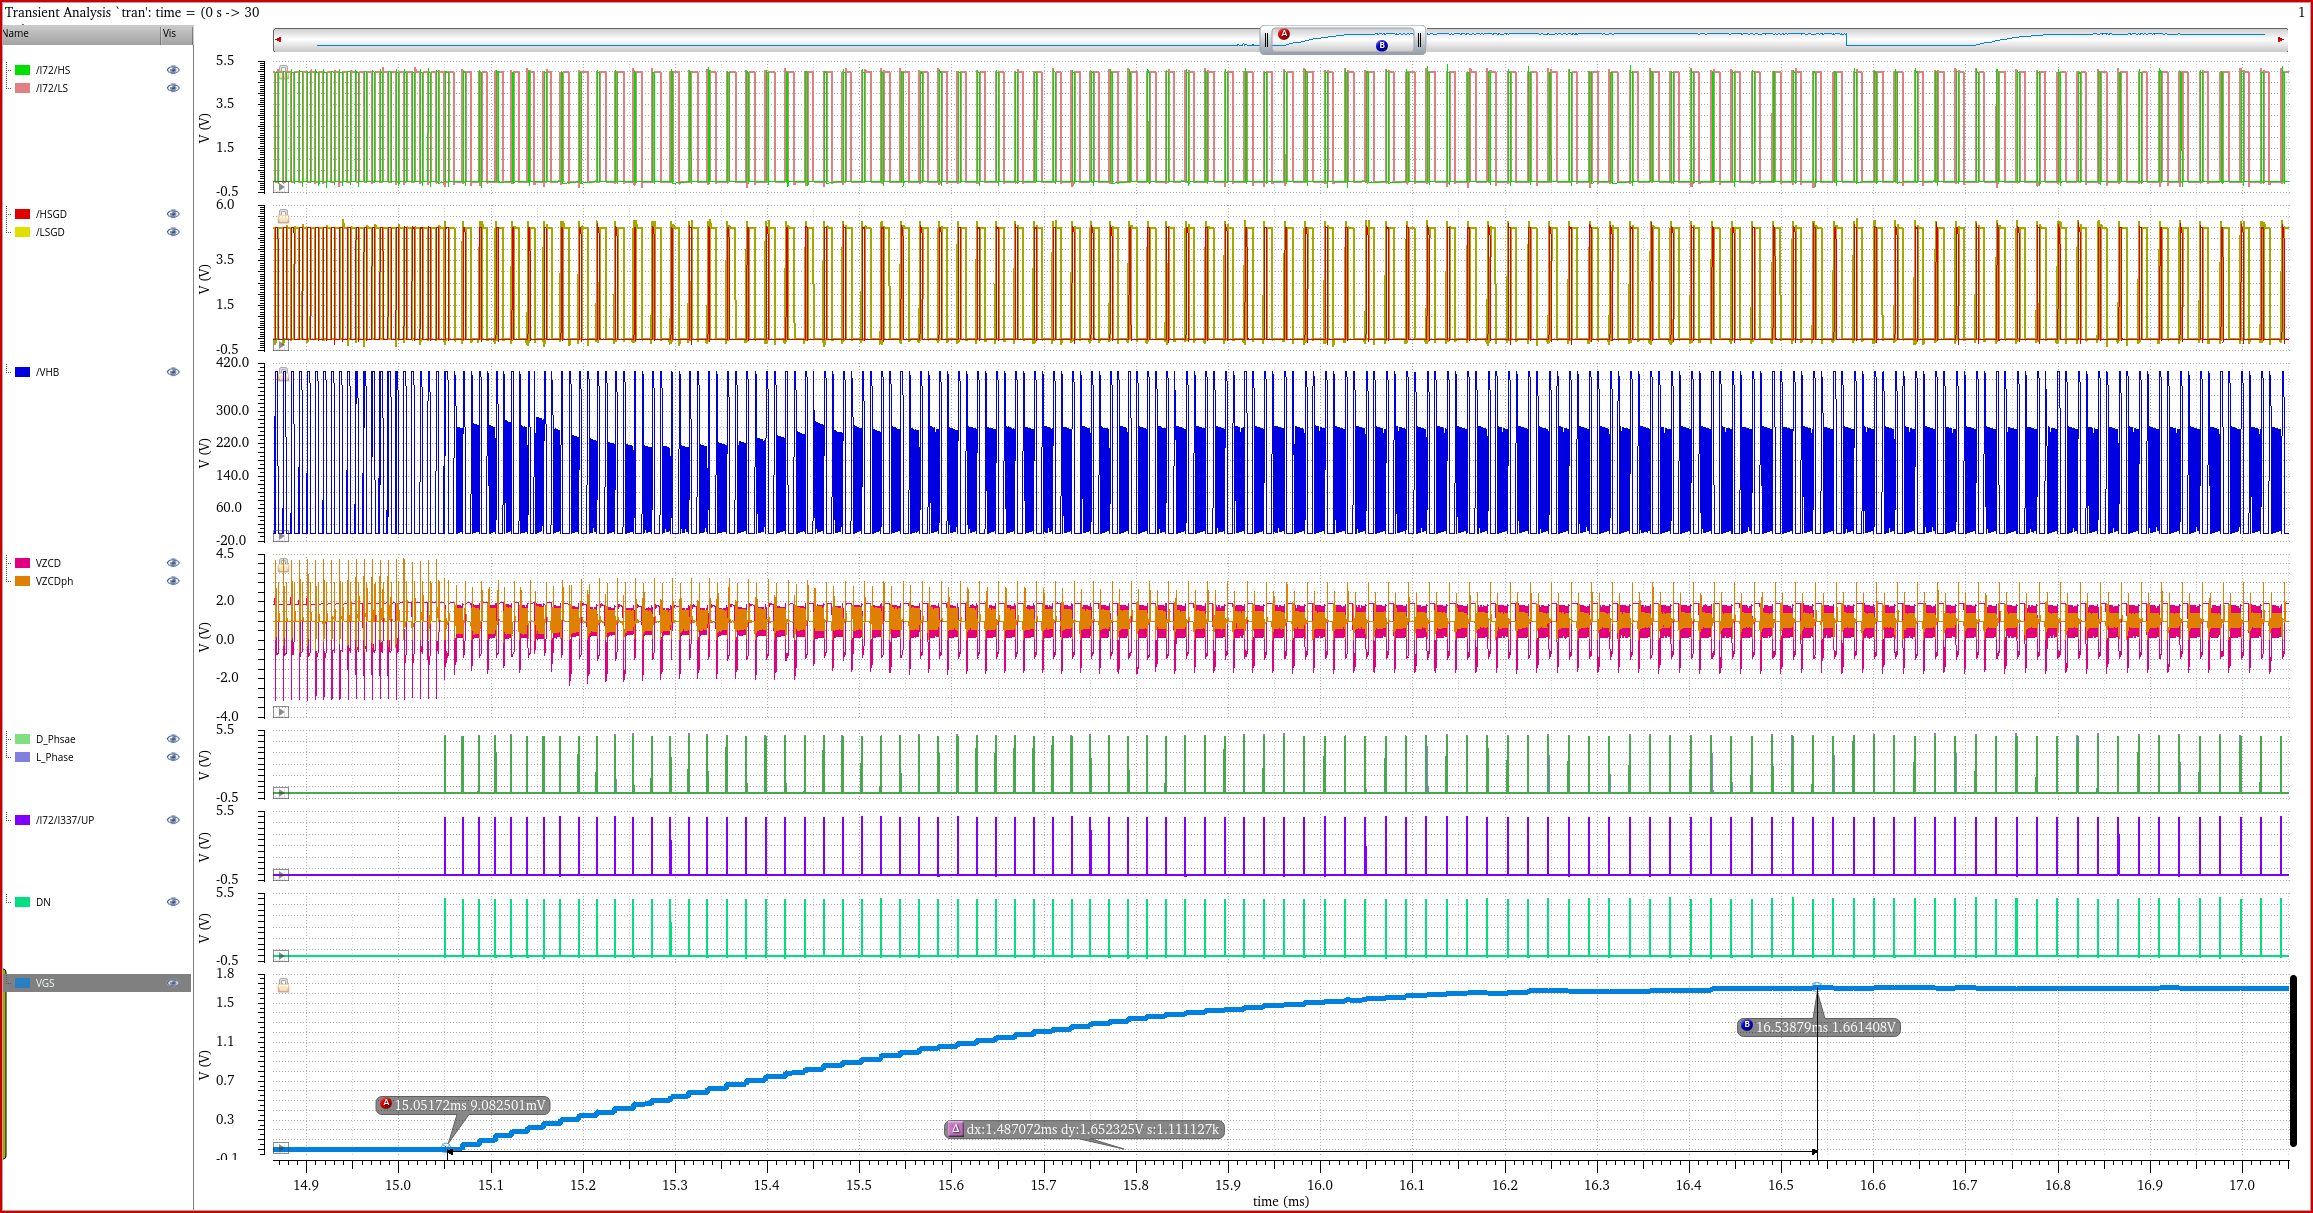
\includegraphics[width=0.8\linewidth]{figures/valley_switch.png}
    \caption{精确谷底导通电路相关波形仿真图}
    \label{fig:谷底导通仿真图}
\end{figure} 

\begin{figure}[H]
	\centering
	\subcaptionbox{未稳定\label{fig:谷底导通仿真图1}}{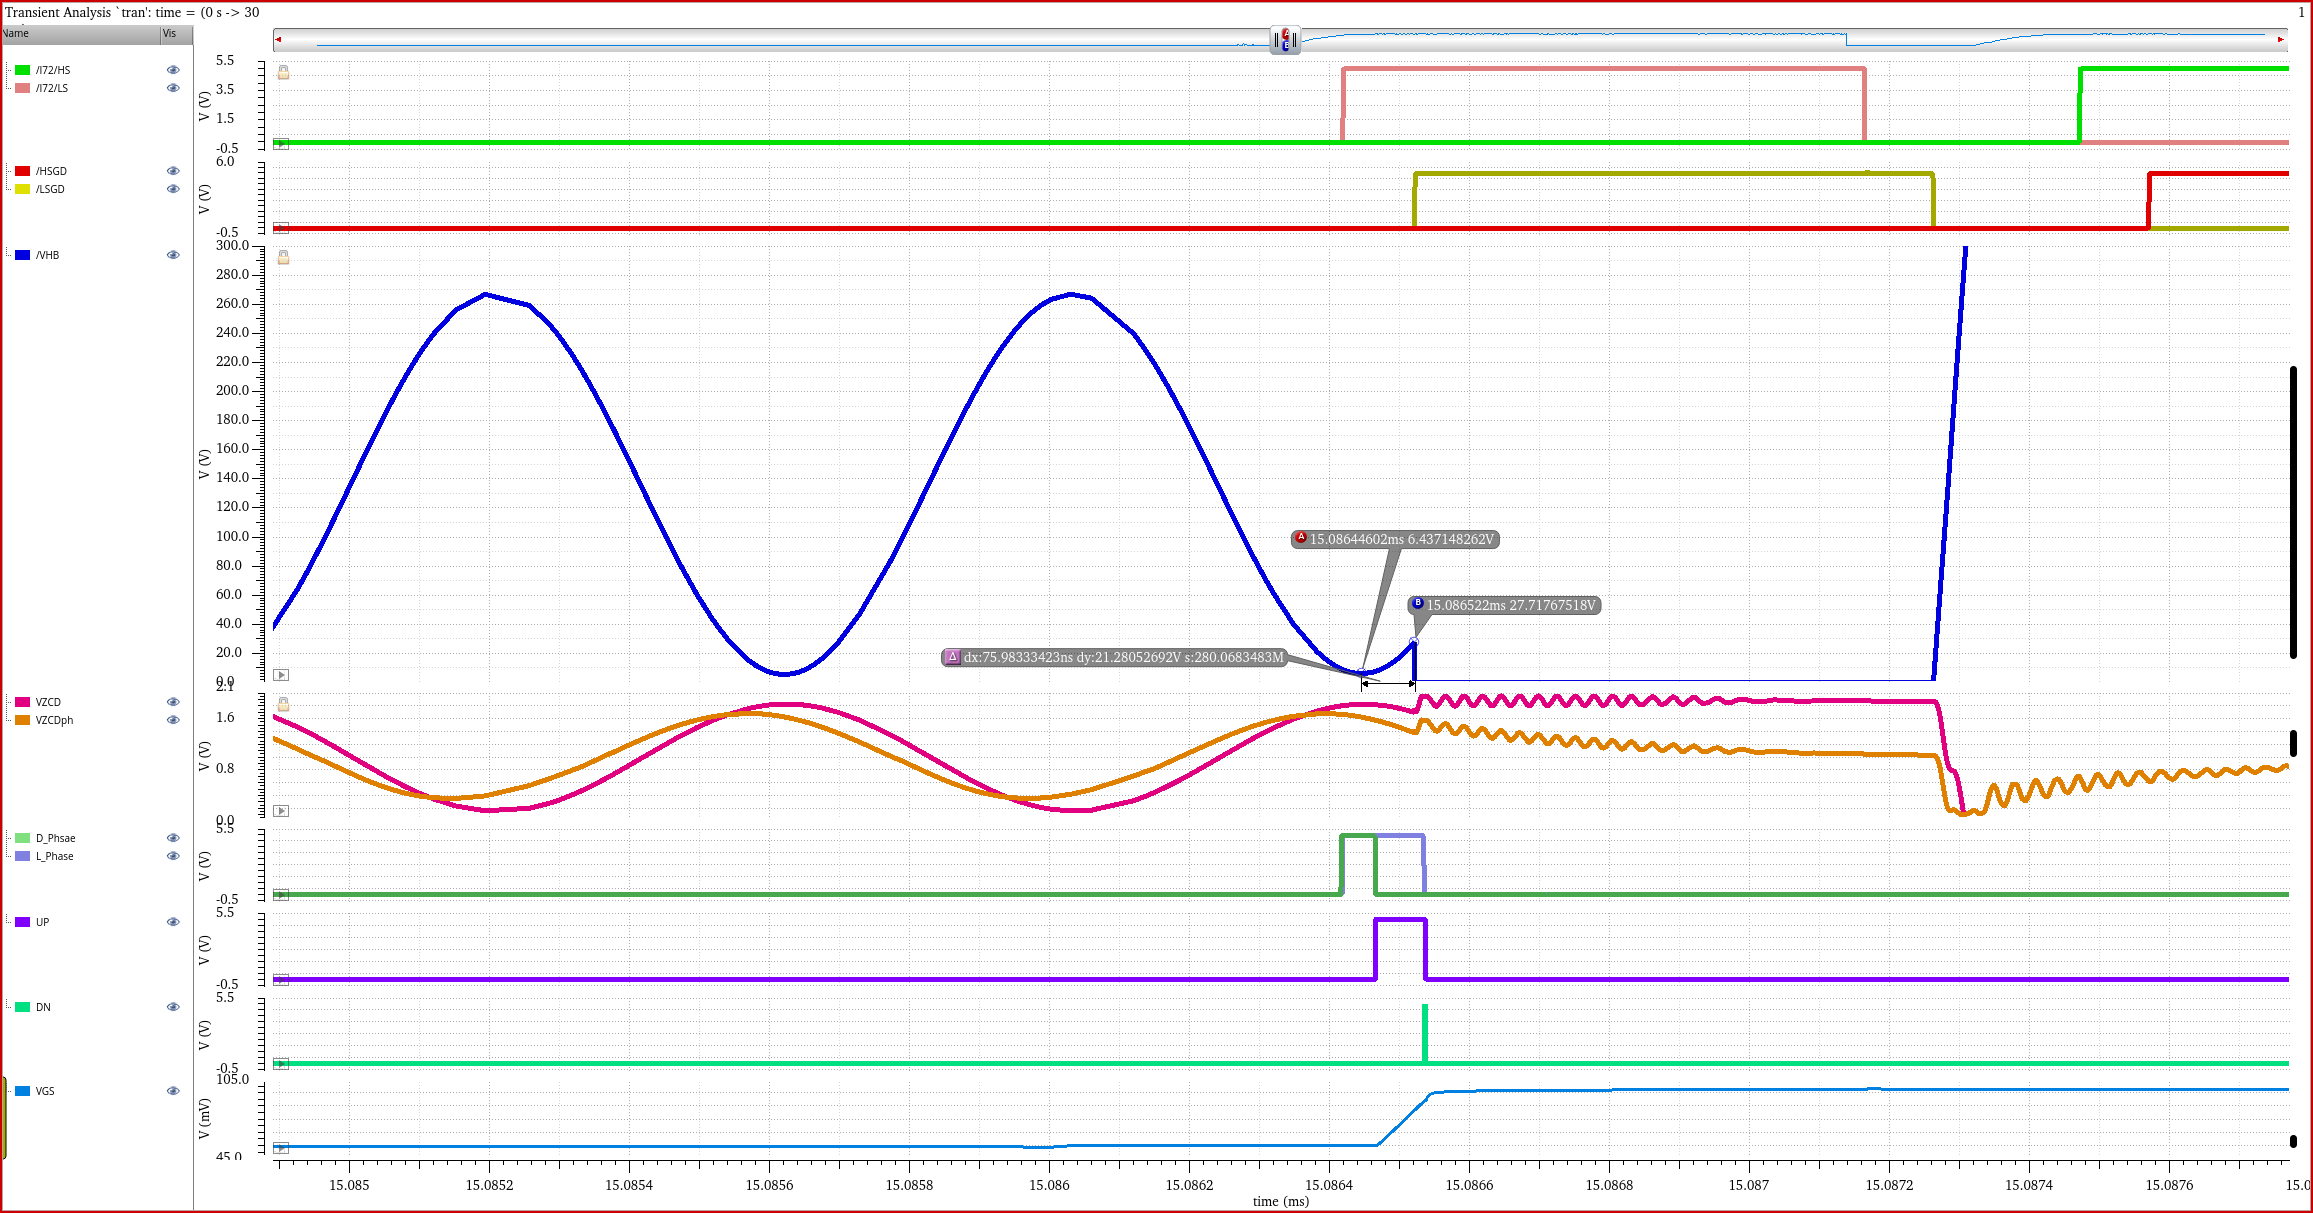
\includegraphics[width = 0.6\linewidth]{figures/valley_switch1.png}}
	\subcaptionbox{稳定\label{fig:谷底导通仿真图2}}{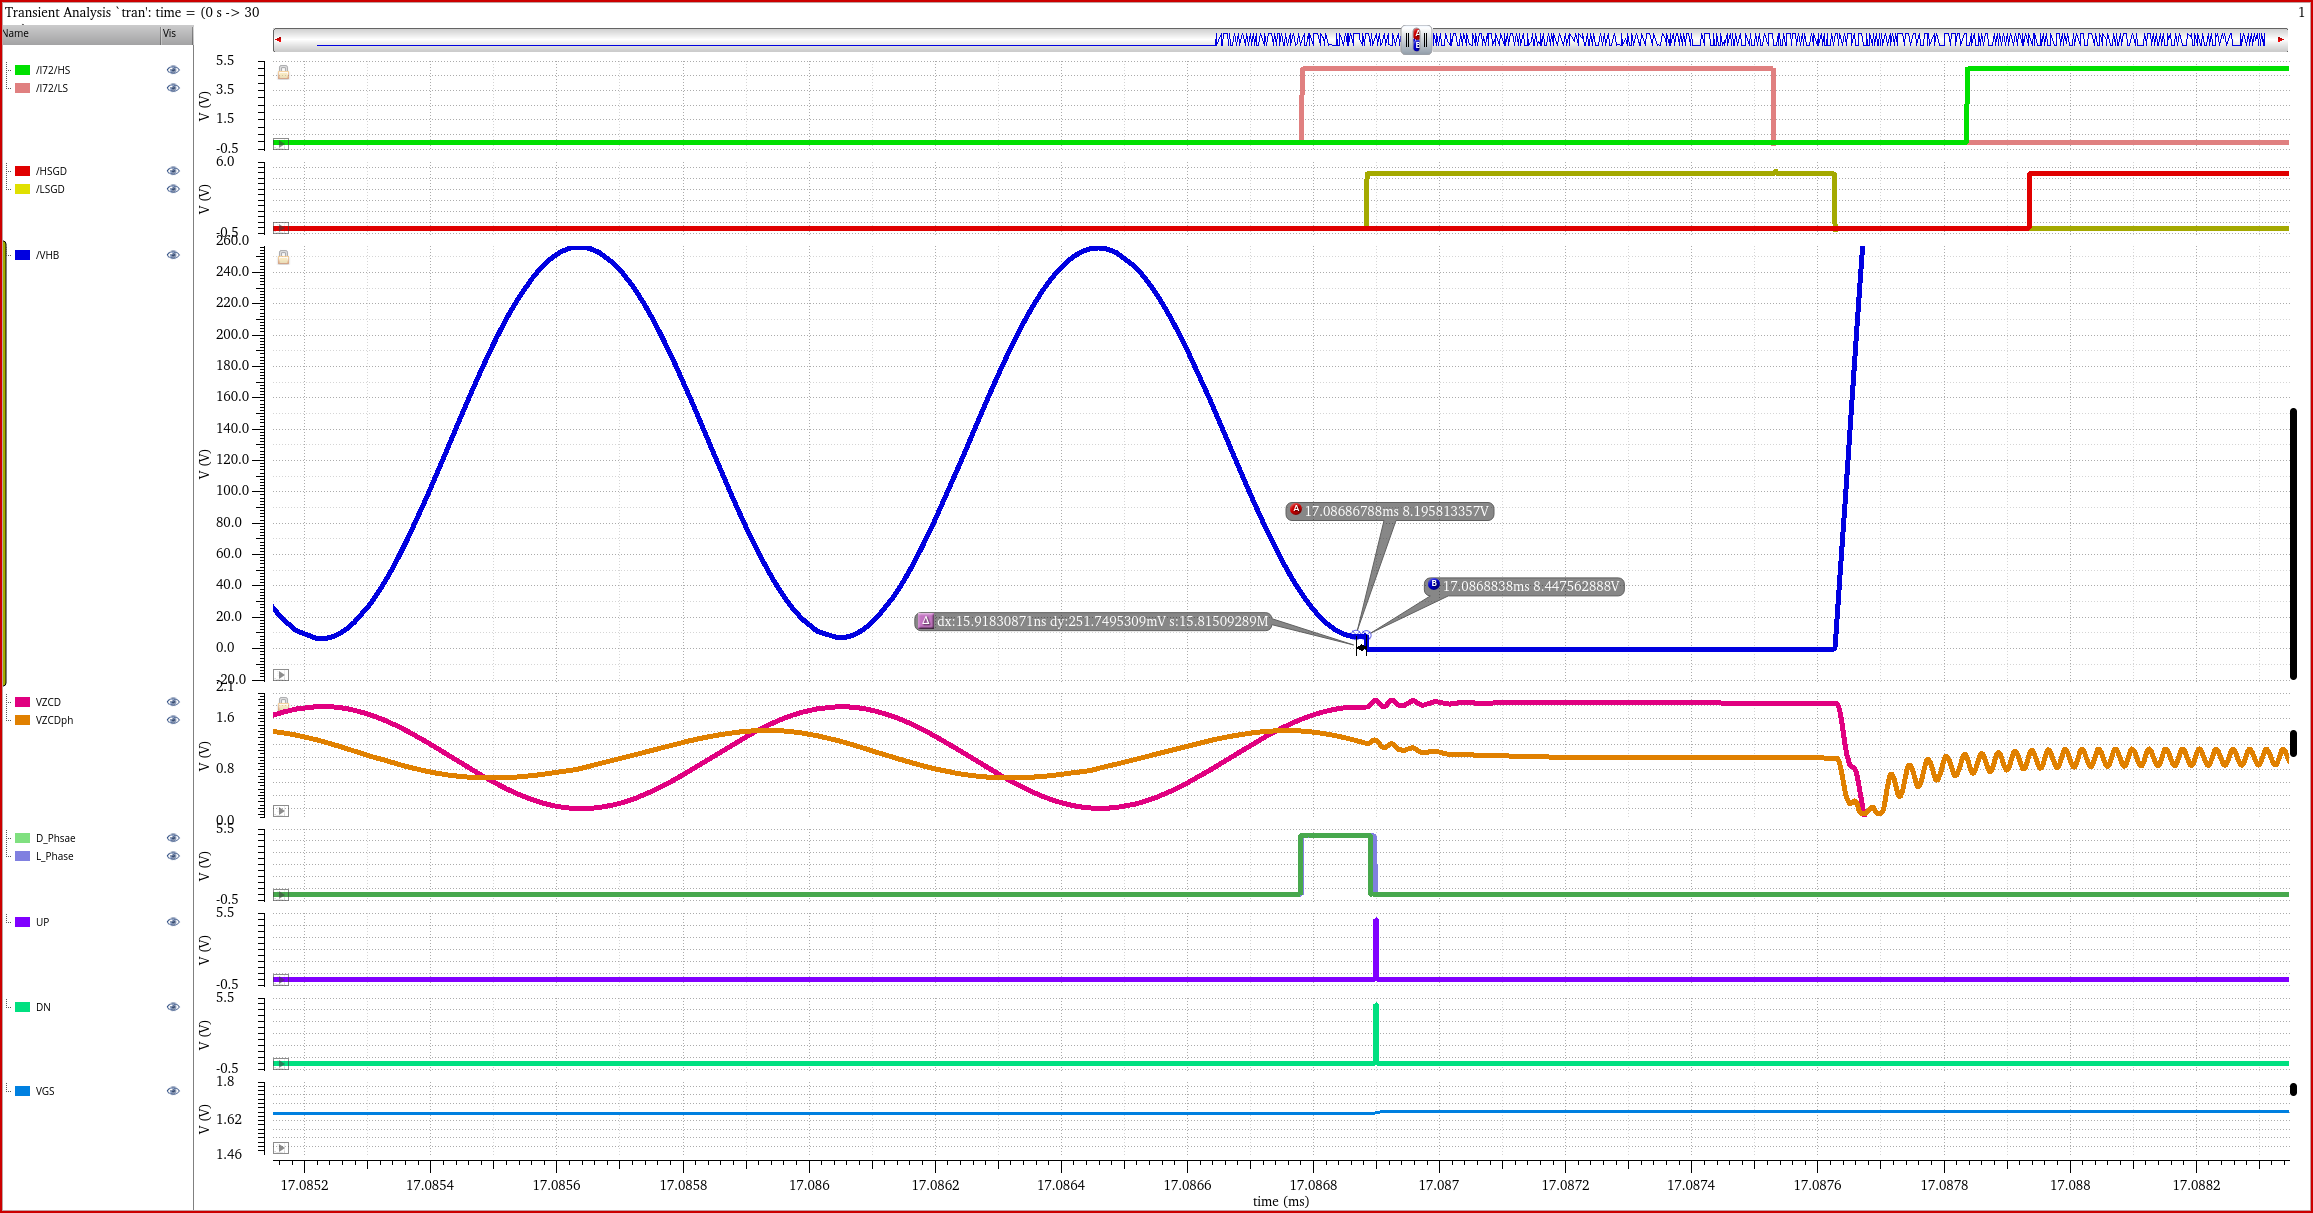
\includegraphics[width = 0.6\linewidth]{figures/valley_switch2.png}}
	\caption{谷底导通放大仿真图}
	\label{fig:谷底导通放大仿真图}
\end{figure}




\section{谷值锁定电路}

\subsection{谷值锁定电路原理}

在RVS工作模式中,上文所提到的精确谷底导通电路工作前需先确认等待时间信号$T_w$,只有识别到$T_w$的下降沿到达后,才能在其之后的谐振谷底处导通低边功率管,如图~\ref{fig:谷值锁定波形1}所示,当t1时刻$T_w$电压由高变低后,精确谷底导通模块开始工作,寻找识别到距离下降沿最近的t2时刻的谐振谷底,开启下个开关周期。

\begin{figure}[htbp] 
    \centering
    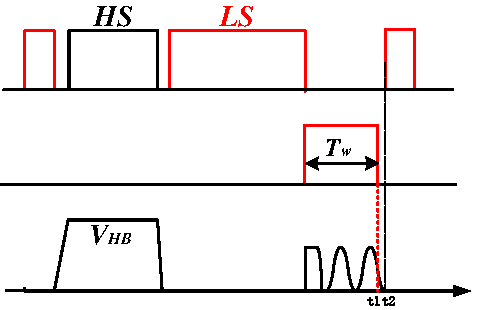
\includegraphics[width=0.8\linewidth]{figures/谷值锁定波形1.pdf}
    \caption{谷值锁定波形1}
    \label{fig:谷值锁定波形1}
\end{figure} 


若使用随负载变化控制频率大小的振荡器电路来产生$T_w$,会出现当输出功率变化到功率重叠范围内时,$T_w$内信号$V_{HB}$的谐振谷数值在不同开关周期内发生来回跳动的情况,称之为跳谷现象,其引起的频率跳变将在这些功率重叠的负载点产生严重的可听噪声。跳谷现象如图~\ref{fig:跳谷现象波形图}所示。其发生的原理是峰值电流电压$V_{CSP}$会随着输出功率的提升而增大,开关周期时间也会同时减小,当输出功率增大到某个点时,控制开关周期开启的时钟信号CLK越过了某个谷底,如图中的CLK1在第一个谷底前产生,此时开关周期从第二个谷底变为了在第一个谷底处开启下一周期,开关频率发生了离散变化,这种突然的变化将导致传输到输出端的功率超过负载的消耗,从而导致输出电压上升。输出电压的增大又会通过反馈回路减小$V_{CSP}$和增大开关周期时间,$T_{sw1}<T_{sw2}$,CLK2又产生在第一个谷底后,致使下一个开关周期在第二谷底处开启,再次发生离散变化,后续开关周期将不停地在第一谷底和第二谷底处开启。
为解决该问题,本文设计了谷值锁定电路。

\begin{figure}[htbp] 
    \centering
    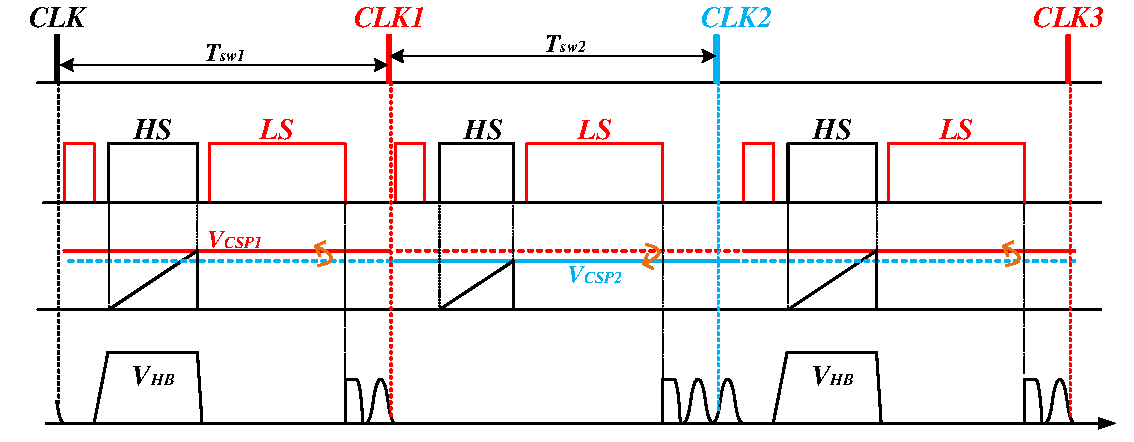
\includegraphics[width=1.0\linewidth]{figures/谷值锁定2.pdf}
    \caption{跳谷现象波形图}
    \label{fig:跳谷现象波形图}
\end{figure} 

谷值锁定电路的作用同样是根据负载的轻重情况调节开关频率大小,副边反馈引脚电压信号$V_{FB}$如~\ref{sec:峰值电流控制电路}小节中提到的,是峰值电流参考电压$V_{CSP}$的重要组成部分,可以一定程度地反映输出负载电流的大小。为了降低导通损耗,需要维持一个较低的峰值电流,因此在负载变化时,利用谷值锁定电路根据$V_{FB}$的变化动态调节谐振谷的数量,以改变$T_w$时间长度的方式改变开关频率,更快地恢复输出电压的稳定。
但不同与振荡器电路的是,为了防止跳谷现象的产生,通过对负载的变化调整并锁定等待时间$T_w$内的谐振谷数值,只有当电路判断实际的谷值和设定谷值相等时,才允许精确谷底导通模块在最近的谷底处导通低边功率管,开启下一开关周期。该电路彻底避免了在负载不变的情况下谐振谷值的频繁变化问题,减小了电路的不稳定现象。

谷值锁定电路具体组成如图~\ref{fig:谷值锁定电路1}所示,主要包括三个迟滞比较器、一个D触发器、一个单向计数器、一个双向计数器和DAC电路等。
%该电路的设计原理是,当输出负载电流较小时,$V_{FB}$的电压值也较小,此时谷值锁定电路增大$T_w$时间内的谐振谷值,降低开关频率。

\begin{figure}[htbp] 
    \centering
    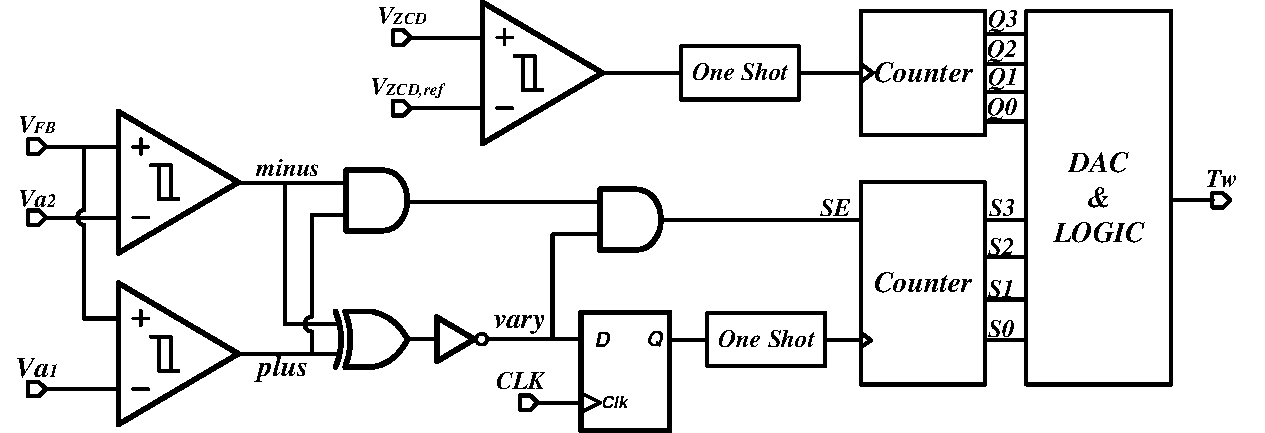
\includegraphics[width=0.8\linewidth]{figures/谷值锁定电路1.pdf}
    \caption{谷值锁定电路1}
    \label{fig:谷值锁定电路1}
\end{figure} 

如图~\ref{fig:谷值变化策略}的谐振谷数值变化策略所示,当输出负载电流较小时,$V_{FB}$电压值小于参考电压Va1,比较器3的输出端plus等于逻辑“1”,此时需要随着CLK信号的触发通过双向计数器电路增加$T_w$时间内的谐振谷数量,降低开关频率;当输出负载电流较大时,$V_{FB}$电压值大于参考电压Va2,比较器2的输出端minus等于逻辑“1”,说明需要减小$T_w$时间内的谐振谷数量,增大开关频率;当$V_{FB}$大于Va1但小于Va2时,锁定$T_w$时间内的谐振谷数量,防止发生跳谷现象。

\begin{figure}[htbp] 
    \centering
    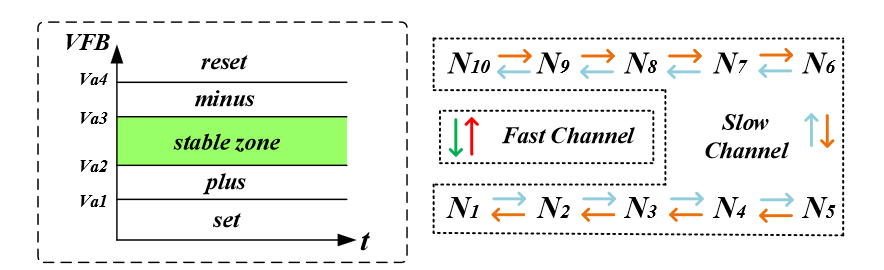
\includegraphics[width=0.8\linewidth]{figures/谷值变化策略.png}
    \caption{谷值变化策略图}
    \label{fig:谷值变化策略}
\end{figure} 

信号$V_{FB}$和参考电压Va1、Va2通过比较器比较后输出的信号plus、minus的组合逻辑决定了谷值锁定电路不同的工作状态,具体工作状态如~\ref{tab:谷值锁定电路}表所示。如在plus信号为逻辑“0”,minus信号为逻辑“1”时,谷值锁定电路将对谐振谷数量进行锁定;在plus和minus信号的其他逻辑转态将对谐振谷进行增加或减小数量的调整操作。plus和minus信号通过一个同或门后输出vary信号并连接到D触发器的D输入端,保证在vary信号为逻辑“1”时允许时钟信号CLK对双向计数器进行计数。plus和minus信号还经过两个与门后输出SE信号,SE信号控制了双向计数器向上和向下的两种计数模式。当SE信号为逻辑“1”时,双向计数器进行向上计数操作,增加$T_w$时间内的谐振谷数量;当SE信号为逻辑“0”时,双向计数器进行向下计数操作,减少$T_w$时间内的谐振谷数量。双向计数器输出的4bit信号S[3:0]会通过DAC电路转为模拟电压信号,与另一个计数器产生的4bit信号Q[3:0]产生的电压信号进行比较,输出$T_w$等待时间给精确谷底导通电路。

其中CLK脉冲信号的设置根据香农定律,为了保证信号采样的完整性,采样频率应至少为带宽的两倍。本文定义$\frac{1}{T_{CLK}}$作为CLK脉冲信号的工作频率。在开关电源系统中,为了避免可听噪声,开关频率$f_{CLK}$必须超过20Hz ~ 20KHz频段。$T_{CLK}$可以表示为如下形式:
\begin{equation}
    \label{eq:CLK公式}
    T_{CLK} > 2 \times \frac{1}{20kHz}
\end{equation}
取$T_{CLK}$的开关周期长度为100u。


%为了防止出现如前文~\ref{sec:多模式切换}小节中提到的峰值电流和开关频率同时变化引起的相位裕度降低和电路不稳定情况,轻载时采取的RVS工作模式通过改变开关频率的方式维持峰值电流的基本恒定。副边反馈引脚电压信号$V_{FB}$如~\ref{sec:峰值电流控制电路}小节中提到的,是峰值电流参考电压$V_{CSP}$的重要组成部分,可以一定程度地反映输出负载电流的大小。当负载电流突然增大时,为了满足变大的输出功率,变压器原边需要增大高边功率管的导通时间提供更多的能量给输出电容,因此$V_{CSP}$增大,$V_{FB}$也相应地增大;当负载电流突然减小时,同理$V_{FB}$也会相应地减小。同时为了降低导通损耗,需要维持一个较低的峰值电流,因此在负载波动时,利用谷值锁定电路通过随$V_{FB}$变化动态调节谐振谷的数量,改变$T_w$时间长度的方式改变开关频率,更快地恢复输出电压的稳定。



\begin{table}[htbp]
    \caption{谷值锁定的三种操作}
    \label{tab:谷值锁定电路}
    \centering
    \belowrulesep=0pt  %防止竖线不连续
    \aboverulesep=0pt  %防止竖线不连续
        \begin{tabular}{|c|c|c|c|c|}
            \toprule
             (minus,plus) & 功能 & vary & SE \\
            \midrule
             (0,0)  & 减小谷值  & 1 &    0                   \\  \midrule
             (0,1)  & 锁定谷值  & 0 & disable                \\  \midrule
             (1,1)  & 增加谷值  & 1 &    1       \\          
            \bottomrule
        \end{tabular}
\end{table}

4bit双向计数器电路的电路图如图~\ref{fig:双向计数器电路}所示,包括四个D触发器和MUX电路。不同于普通的单向计数器,可以通过SE信号选择实现向上或向下计数的功能。当SE信号为逻辑“1”时,将每个D触发器的反向输出端输入到下一个D触发器的CLK输入端,此时是向上计数功能;当SE信号为逻辑“0”时,MUX将D触发器的正向输出端输入到下一个D触发器的CLK输入端,实现向下计数功能。电路中还包括hold信号,hold信号的作用是消隐掉SE信号的电平切换的上升沿或下降沿,防止其对计数方向切换造成影响。

\begin{figure}[htbp] 
    \centering
    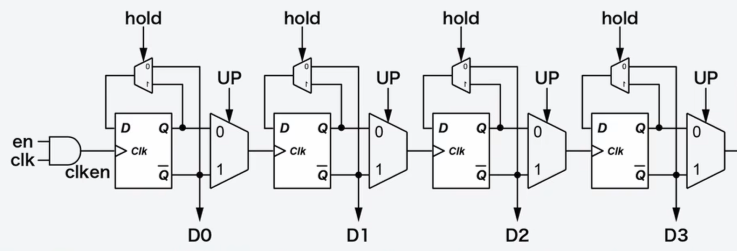
\includegraphics[width=0.8\linewidth]{figures/双向计数器电路.png}
    \caption{双向计数器电路图}
    \label{fig:双向计数器电路}
\end{figure} 

谷值锁定电路中的DAC电路如图~\ref{fig:双向计数器电路}所示,计数器的计数值作为DAC的输入信号,两个计数器分别控制思路电流镜开关管的导通和关断,每个电流镜的镜像比例为1:2:4:8,成倍增加,产生随4bit数字信号S[3:0]、Q[3:0]信号对应的电流$I_S$、$I_Q$。电流镜采用了cascode结构增大电流镜的输出阻抗,提高电流镜像的精度。每一路电流镜还都添加了毛刺消除结构晶体管M11、M13等,用于吸收当数字信号控制M10、M12等开关管导通瞬间产生的巨大毛刺电压。
没有毛刺消除结构时,如图~\ref{fig:双向计数器电路}中的电压V2和V3,分别为晶体管M2和M3的漏极电压,在数字信号S0未导通开关管M10时,$V_2=V_3=V_{DD}$;当S0控制开关管M10导通,电压V3由于cascode结构的大输出阻抗的作用下和电压V1近似相等,电压V2则由于开关管导通等于电阻$R_S$上的电压。在开关管通断前后电压V2和V3的变化量分别为:
\begin{equation}
    \label{eq:△V2公式}
    \varDelta V_2 = V_{DD} - V_{GS1}
\end{equation}
\begin{equation}
    \label{eq:△V3公式}
    \varDelta V_3 = V_{DD} - V_S
\end{equation}

由于电流镜晶体管存在寄生电容$C_{ds}$,故电流镜晶体管M3和M2的寄生电容上的能量$\varDelta P_3 = \varDelta V_3 C_{ds3}$、$\varDelta P_2 = \varDelta V_2 C_{ds2}$会在开关管导通的瞬间传递到电阻$R_S$上,在电压$V_S$引起巨大的毛刺。加入毛刺消除结构M11后,由于M11是NMOS晶体管,其会和开关管M10交替导通,在晶体管M11导通时,电压V2等于零,电压V3的值仍近似等于V1;当开关管M10导通的时候,电压V2和V3的值和没有晶体管M11时相同,故电压V2和V3的变化量分别变为:
\begin{equation}
    \label{eq:△V2公式1}
    \varDelta V_2 = V_{GS1} - V_{GS1} = 0
\end{equation}
\begin{equation}
    \label{eq:△V3公式1}
    \varDelta V_3 = V_S - 0 = V_S
\end{equation}
由式中可见得,电压V2和V3的变化量大大降低,明显降低了毛刺现象。

\begin{figure}[htbp] 
    \centering
    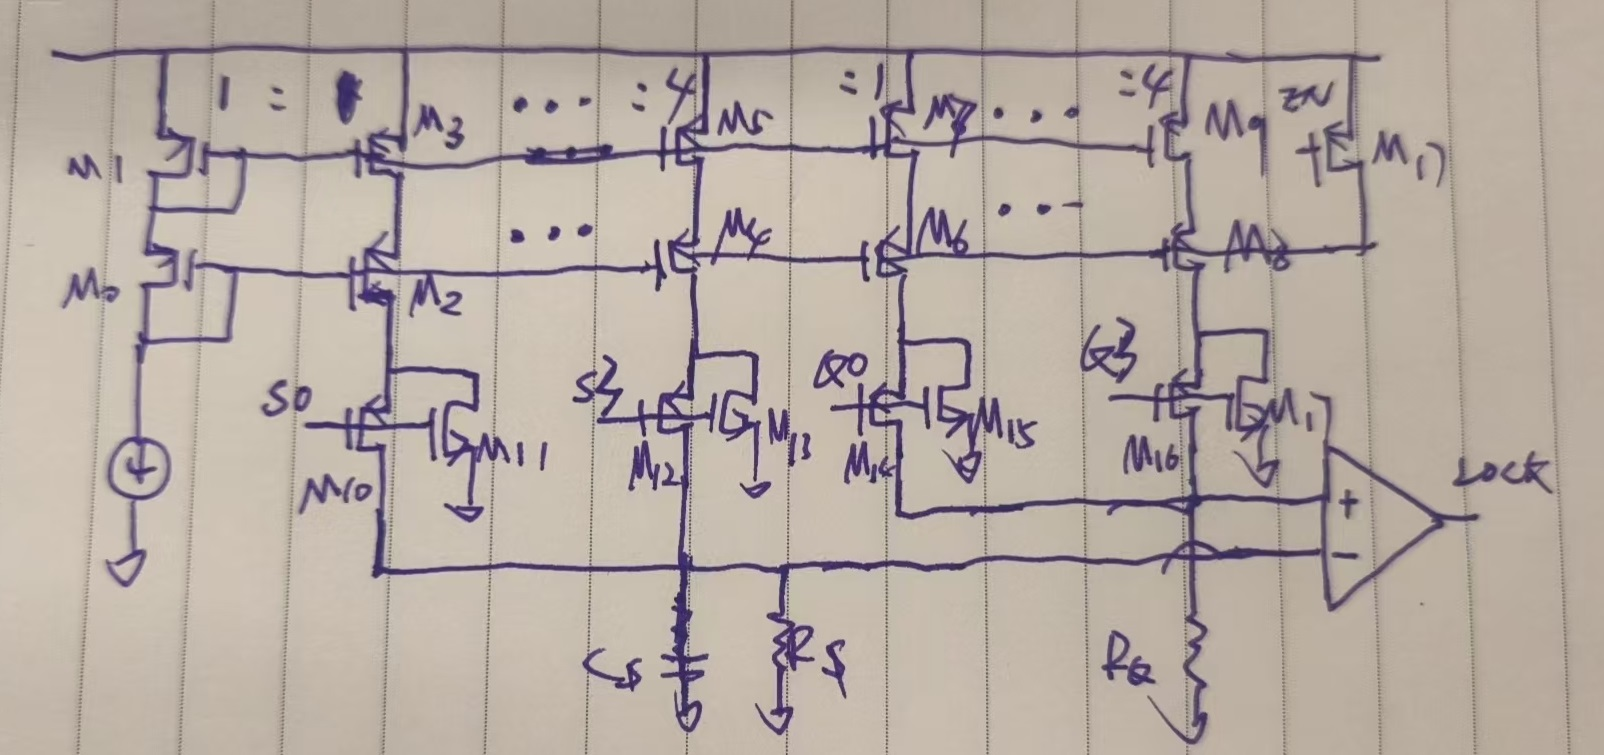
\includegraphics[width=0.6\linewidth]{figures/DAC电路.jpg}
    \caption{DAC电路图}
    \label{fig:DAC电路}
\end{figure} 

数字信号S[3:0]、Q[3:0]控制产生的电流$I_S$、$I_Q$流经电阻$R_S$、$R_Q$后产生的电压$V_S$、$V_Q$通过比较器进行比较大小,当电压$V_Q$大于$V_S$后,比较器输出信号$T_w$由高电平转为低电平,锁定时间结束,精确谷底导通电路开始工作,寻找最近的谐振谷底开启下一开关周期。

\subsection{谷值锁定电路仿真分析}

\begin{figure}[htbp] 
    \centering
    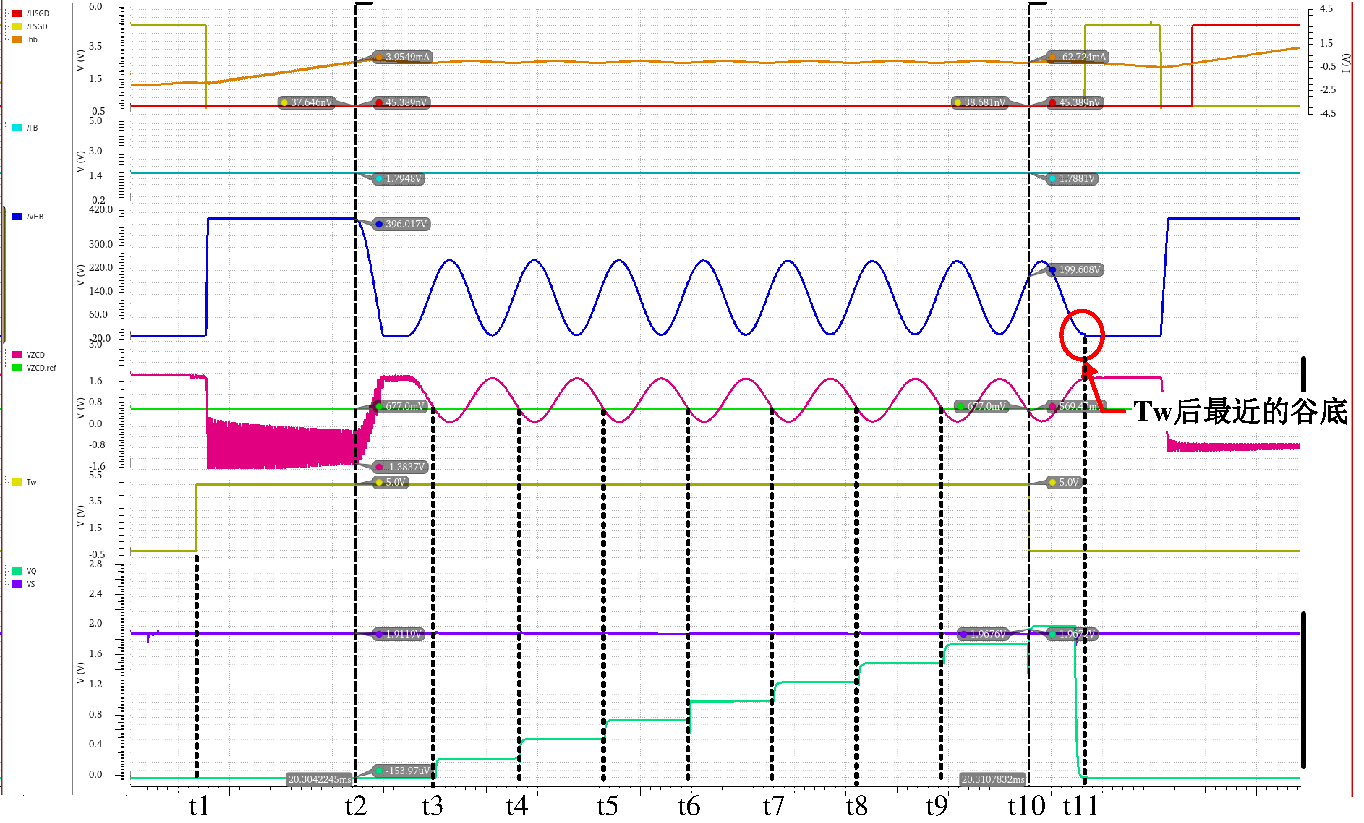
\includegraphics[width=0.8\linewidth]{figures/valley_lock.pdf}
    \caption{单周期谷值锁定电路波形图}
    \label{fig:单周期谷值锁定电路波形图}
\end{figure} 

图~\ref{fig:单周期谷值锁定电路波形图}为单个开关周期内的谷值锁定电路相关的波形图,图中在t1时刻处,原边励磁电感退磁完成,低边功率管顺势关断,此时进入等待时间$T_w$内,图中$T_w$的波形由低电平变化为高电平,在经过一段时间在t2时刻原边电流恢复到零安培后,半桥节点电压信号$V_{FB}$和辅助绕组分压信号$V_{ZCD}$开始自由振荡,通过比较$V_{ZCD}$和$V_{ZCD,ref}$的电压值大小,计数器1不断地对谐振谷进行计数,并通过DAC电路输出电压信号$V_{Q}$,在图中可见在t3、t4、t5等时刻电压$V_{Q}$的波形持续进行阶梯式的抬升,直至在t10时刻大于电压信号$V_{S}$,完成信号$V_{S}$设置的八个谷值的锁定功能,$T_w$的波形同时也由高电平变化为低电平,精确谷底导通电路采样到此下降沿后,在t11时刻的第八个谐振谷底处开启下一个开关周期。


图~\ref{fig:多周期谷值锁定电路波形图}为多个开关周期内的谷值锁定电路相关的波形图,输出负载电流在图中从1A在t1时刻变化为1.5A,在t5时刻再次变化2A。随着输出负载电流的变化,信号$V_{FB}$的波形如上文所提到的,相应地发生变化。在t1时刻前,$V_{FB}$小于参考电压$V_{a1}$,此时图中的信号vary为逻辑“1”的高电平,信号SE为逻辑“0”的低电平,表示此时计数器应该随着信号CLK的脉冲增加谐振谷数值,但由于此时图中谐振谷数值已经达到最大谷值,故参考电压$V_S$未发生变化保持恒定的3.15V。
在t1时刻后,负载电流增大为1.5A,在开关频率未变化的情况下,$V_{FB}$为满足输出功率的需求,迅速增大,在t3时刻爬升到大于参考电压$V_{a2}$,信号vary为逻辑“1”,信号SE同样为逻辑“1”,此状态计数器应减少谐振谷数值,在t3和t4时刻之间,随着CLK的脉冲信号电压$V_S$呈阶梯式降低,开关周期每100us缩短一个谐振谷长度,持续增大开关频率,进而降低$V_{FB}$的电压值以维持一个较低的峰值电流。
在t4时刻处,$V_{FB}$降低至小于参考电压$V_{a2}$,信号vary变为逻辑“0”并disable信号SE,谐振谷数值不再发生变化,$V_{FB}$的电压值稳定在1.722V,直至t5时刻负载电流再次增大,后续波形的变化同理。

\begin{figure}[htbp] 
    \centering
    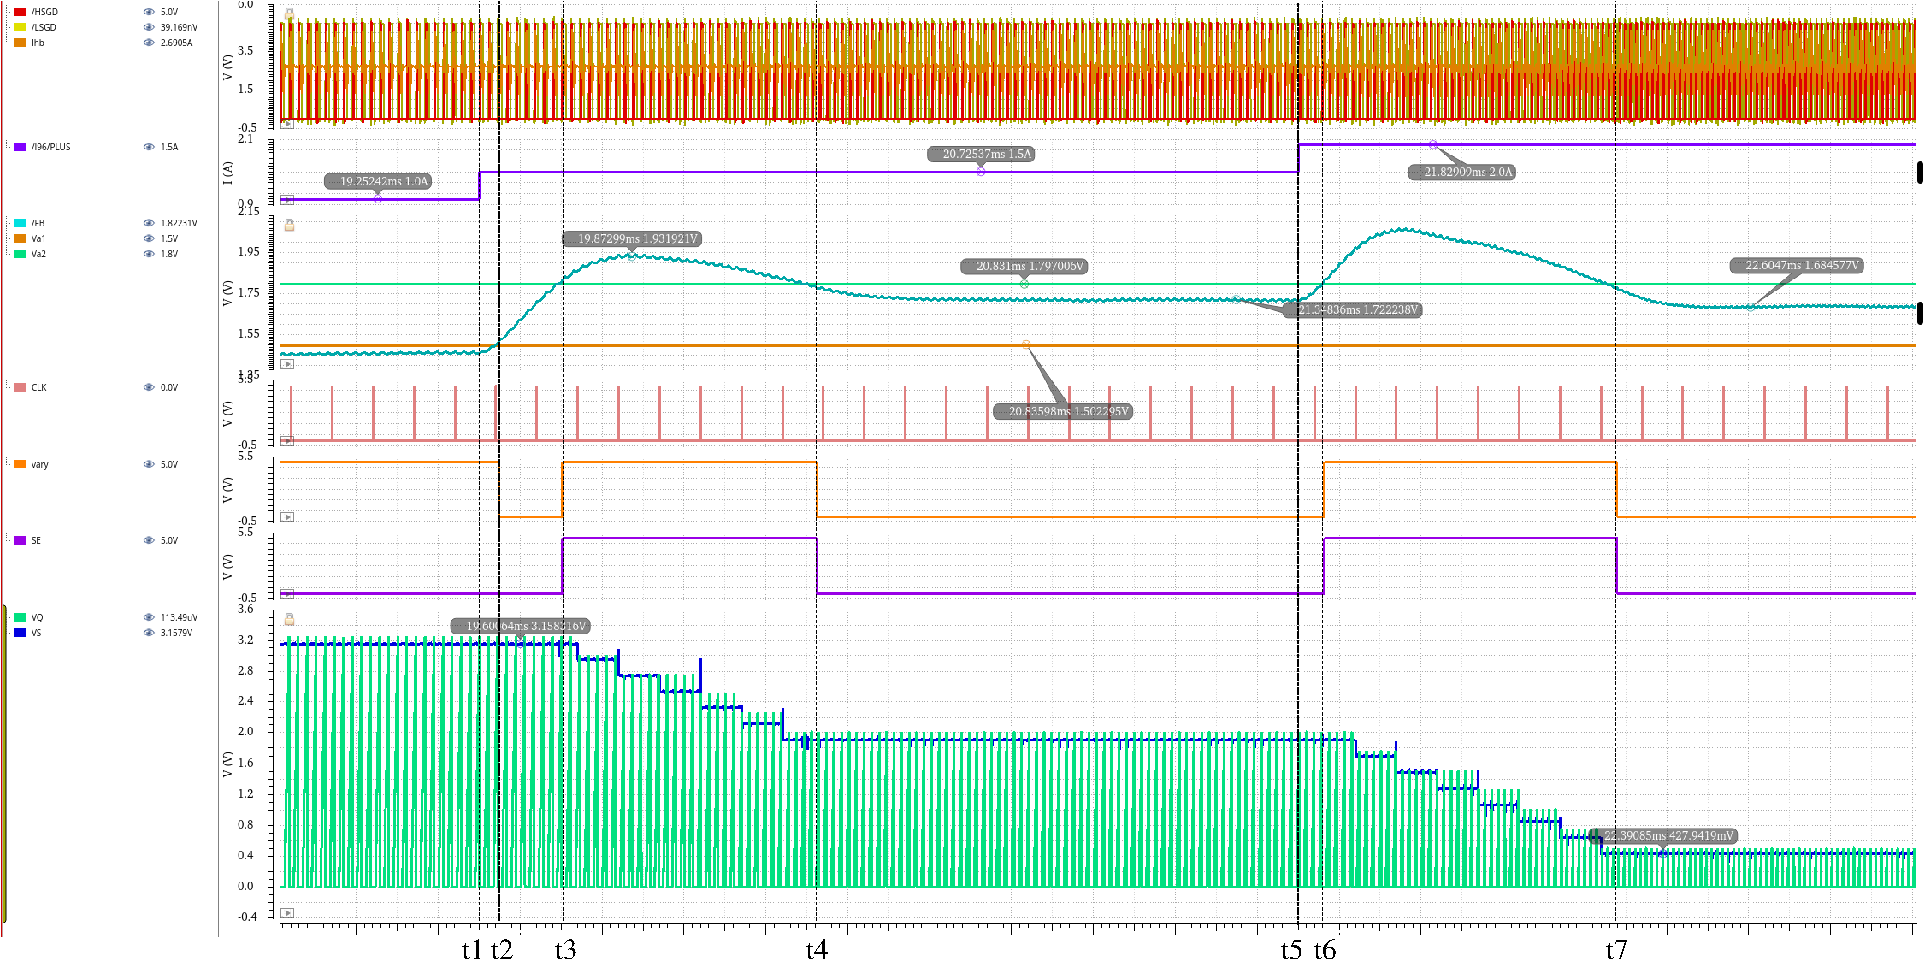
\includegraphics[width=0.8\linewidth]{figures/valley_lock1.pdf}
    \caption{多周期谷值锁定电路波形图}
    \label{fig:多周期谷值锁定电路波形图}
\end{figure} 

图~\ref{fig:谷值锁定放大仿真图}是具体不同负载下谷值锁定电路的仿真波形图。当系统在1.5A的负载电流下稳定后,如图~\ref{fig:多周期谷值锁定电路波形图}中的t4-t5时间段内,谷值锁定电路将每个开关周期内等待时间的谐振谷锁定在相同数值,防止跳谷现象的发生,在图~\ref{fig:谷值锁定仿真图1}中可见得,连续5个开关周期内都保持在第八个谐振谷底处导通低边功率管,未发生跳谷现象。在图~\ref{fig:谷值锁定仿真图2}中可,在2A的负载电流情况下,稳定后的系统在每个开关周期内的第二个谐振谷底处导通低边功率管,同样未发生跳谷现象。

\begin{figure}[htbp]
	\centering
	\subcaptionbox{1.5A负载\label{fig:谷值锁定仿真图1}}{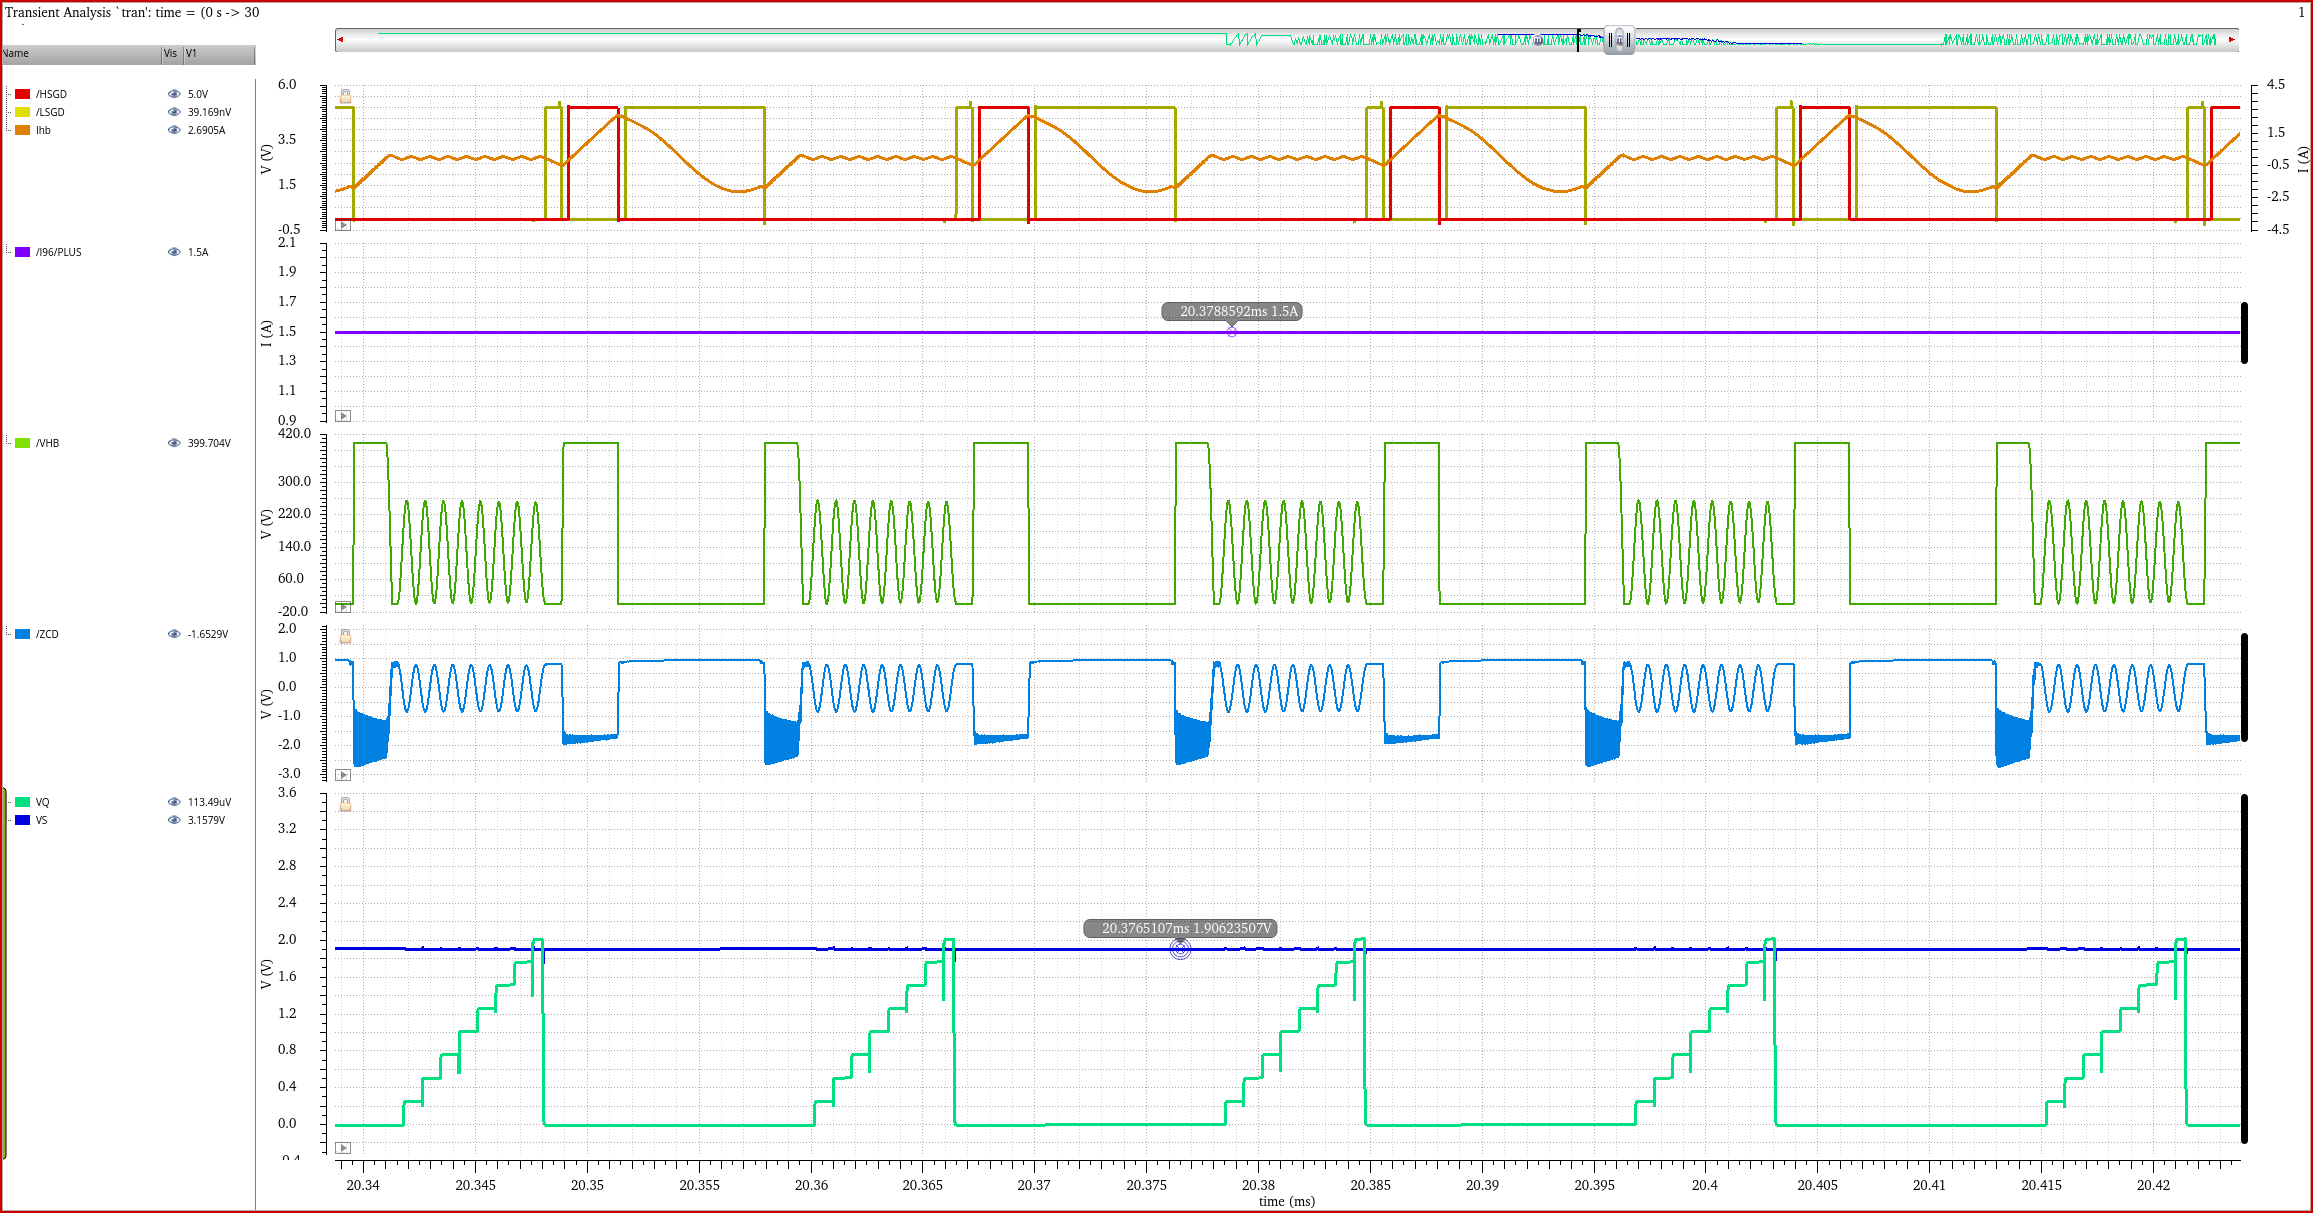
\includegraphics[width = 0.6\linewidth]{figures/valley_lock1.5A.png}}
	\subcaptionbox{2A负载  \label{fig:谷值锁定仿真图2}}{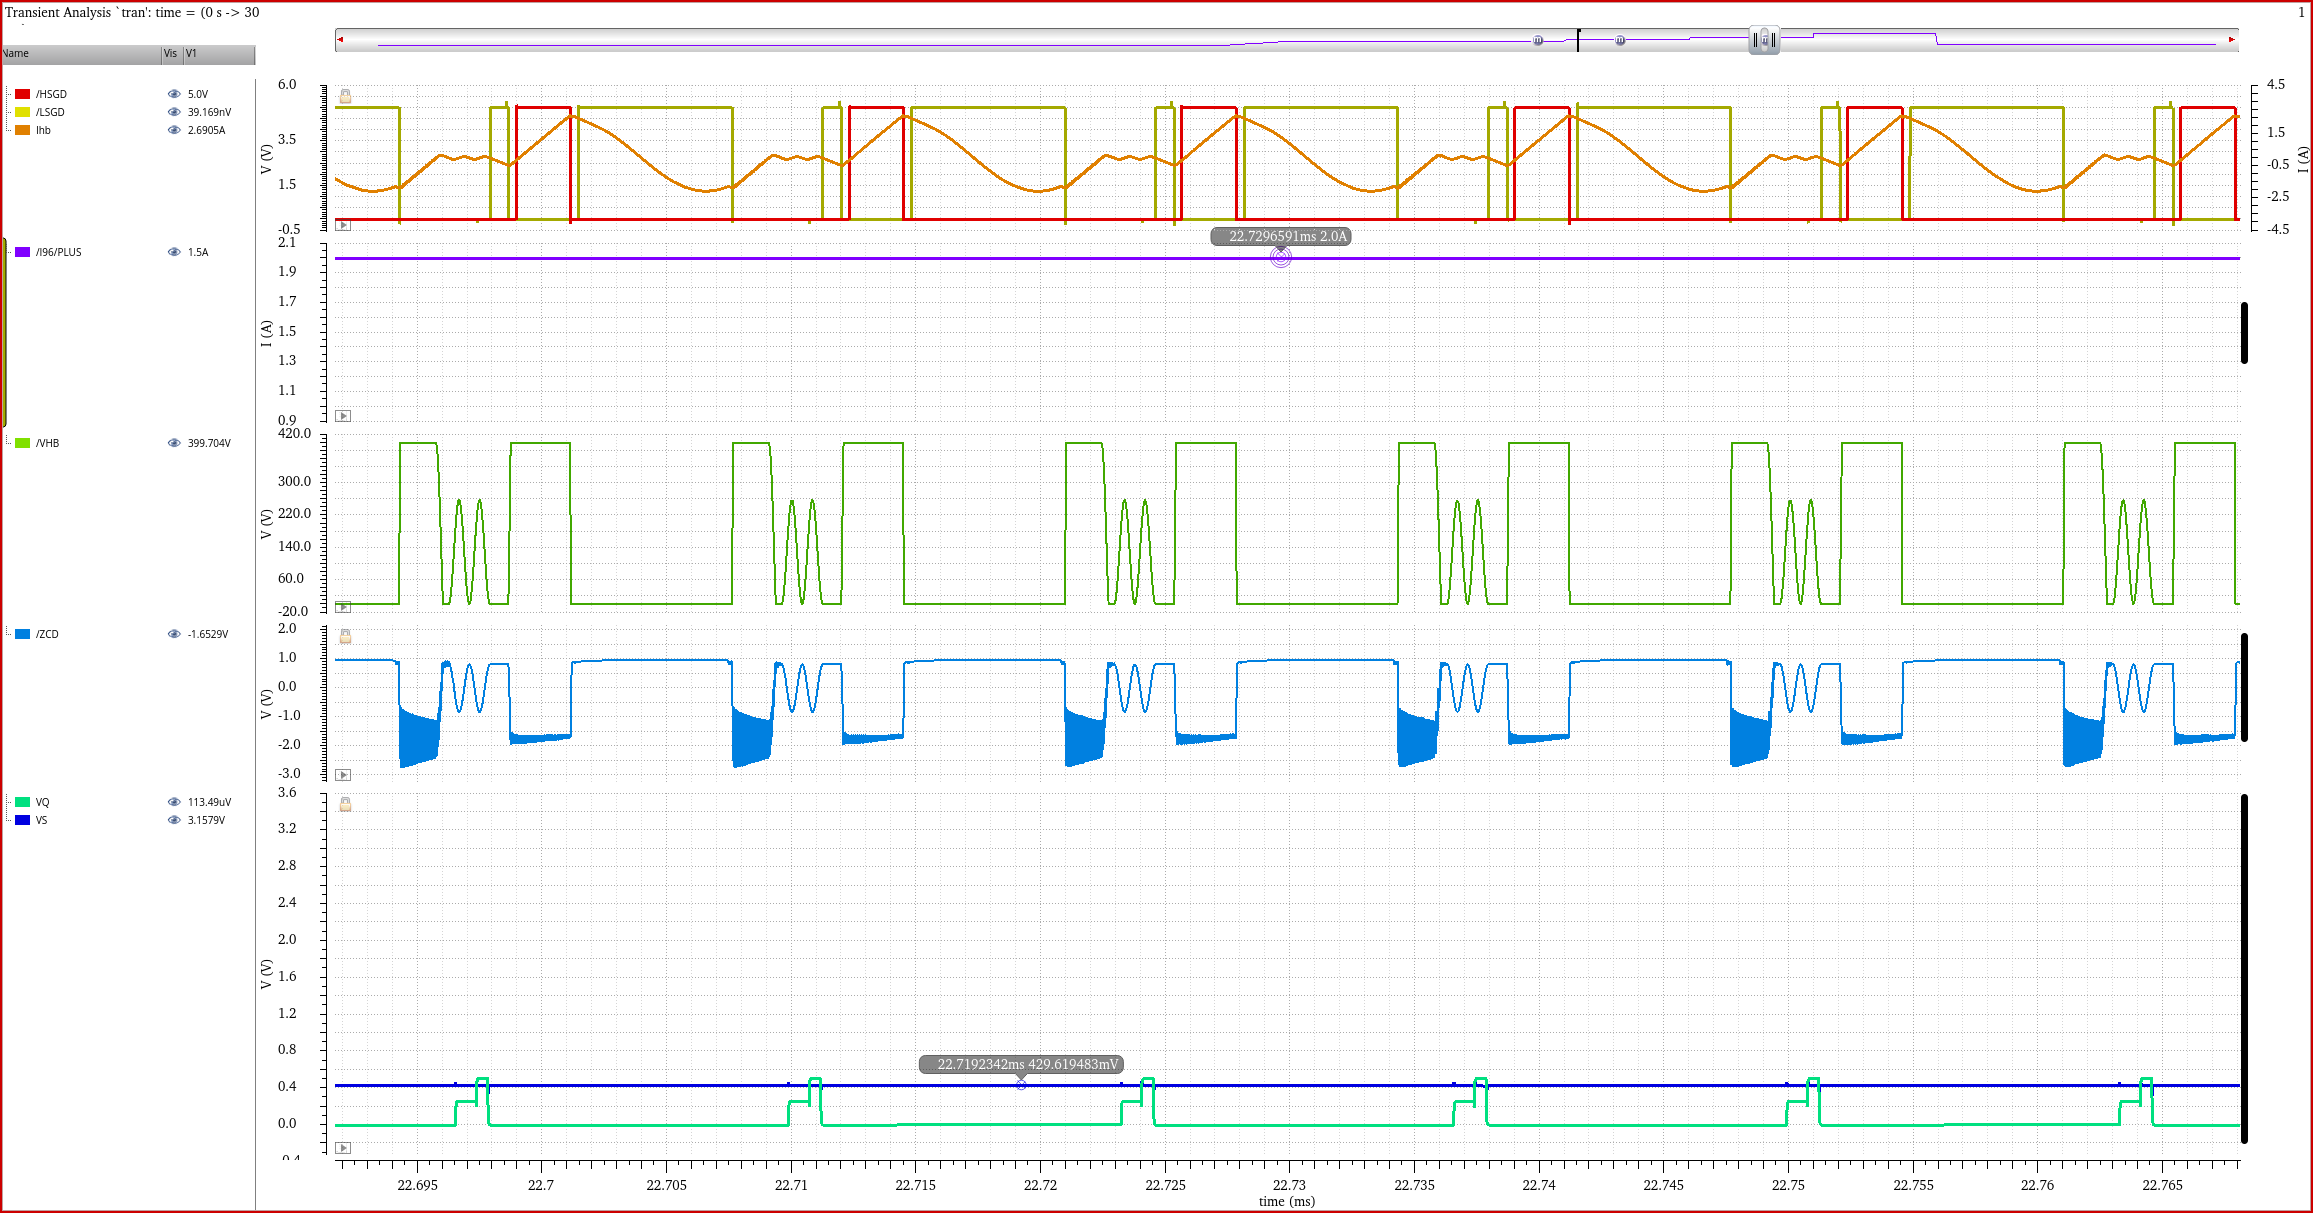
\includegraphics[width = 0.6\linewidth]{figures/valley_lock2A.png}}
	\caption{不同负载谷值锁定仿真图}
	\label{fig:谷值锁定放大仿真图}
\end{figure}

该谷值锁定电路还加入了谷值快切换的功能,不同于前文提到的谷值数量随着时钟信号逐个增加或减少,在快切换功能中,当判断到
$V_{FB}$的电压值迅速超过$V_{a3}$或低于$V_{a0}$时,判断该情况为负载较大的变化,此时谷值数量将被电路直接置位到最大谷值数量或复位到最小谷值数量,以快速变化为到对应负载电流所匹配的开关频率,实现快速响应的功能。



如图~\ref{fig:快慢切换的谷值锁定仿真图}中所示显示了在不同程度负载电流跳变引起的快慢切换策略的谷值锁定电路仿真图。

\begin{figure}[htbp]
	\centering
	\subcaptionbox{1.5A-2A  \label{fig:谷值锁定慢切换仿真}}{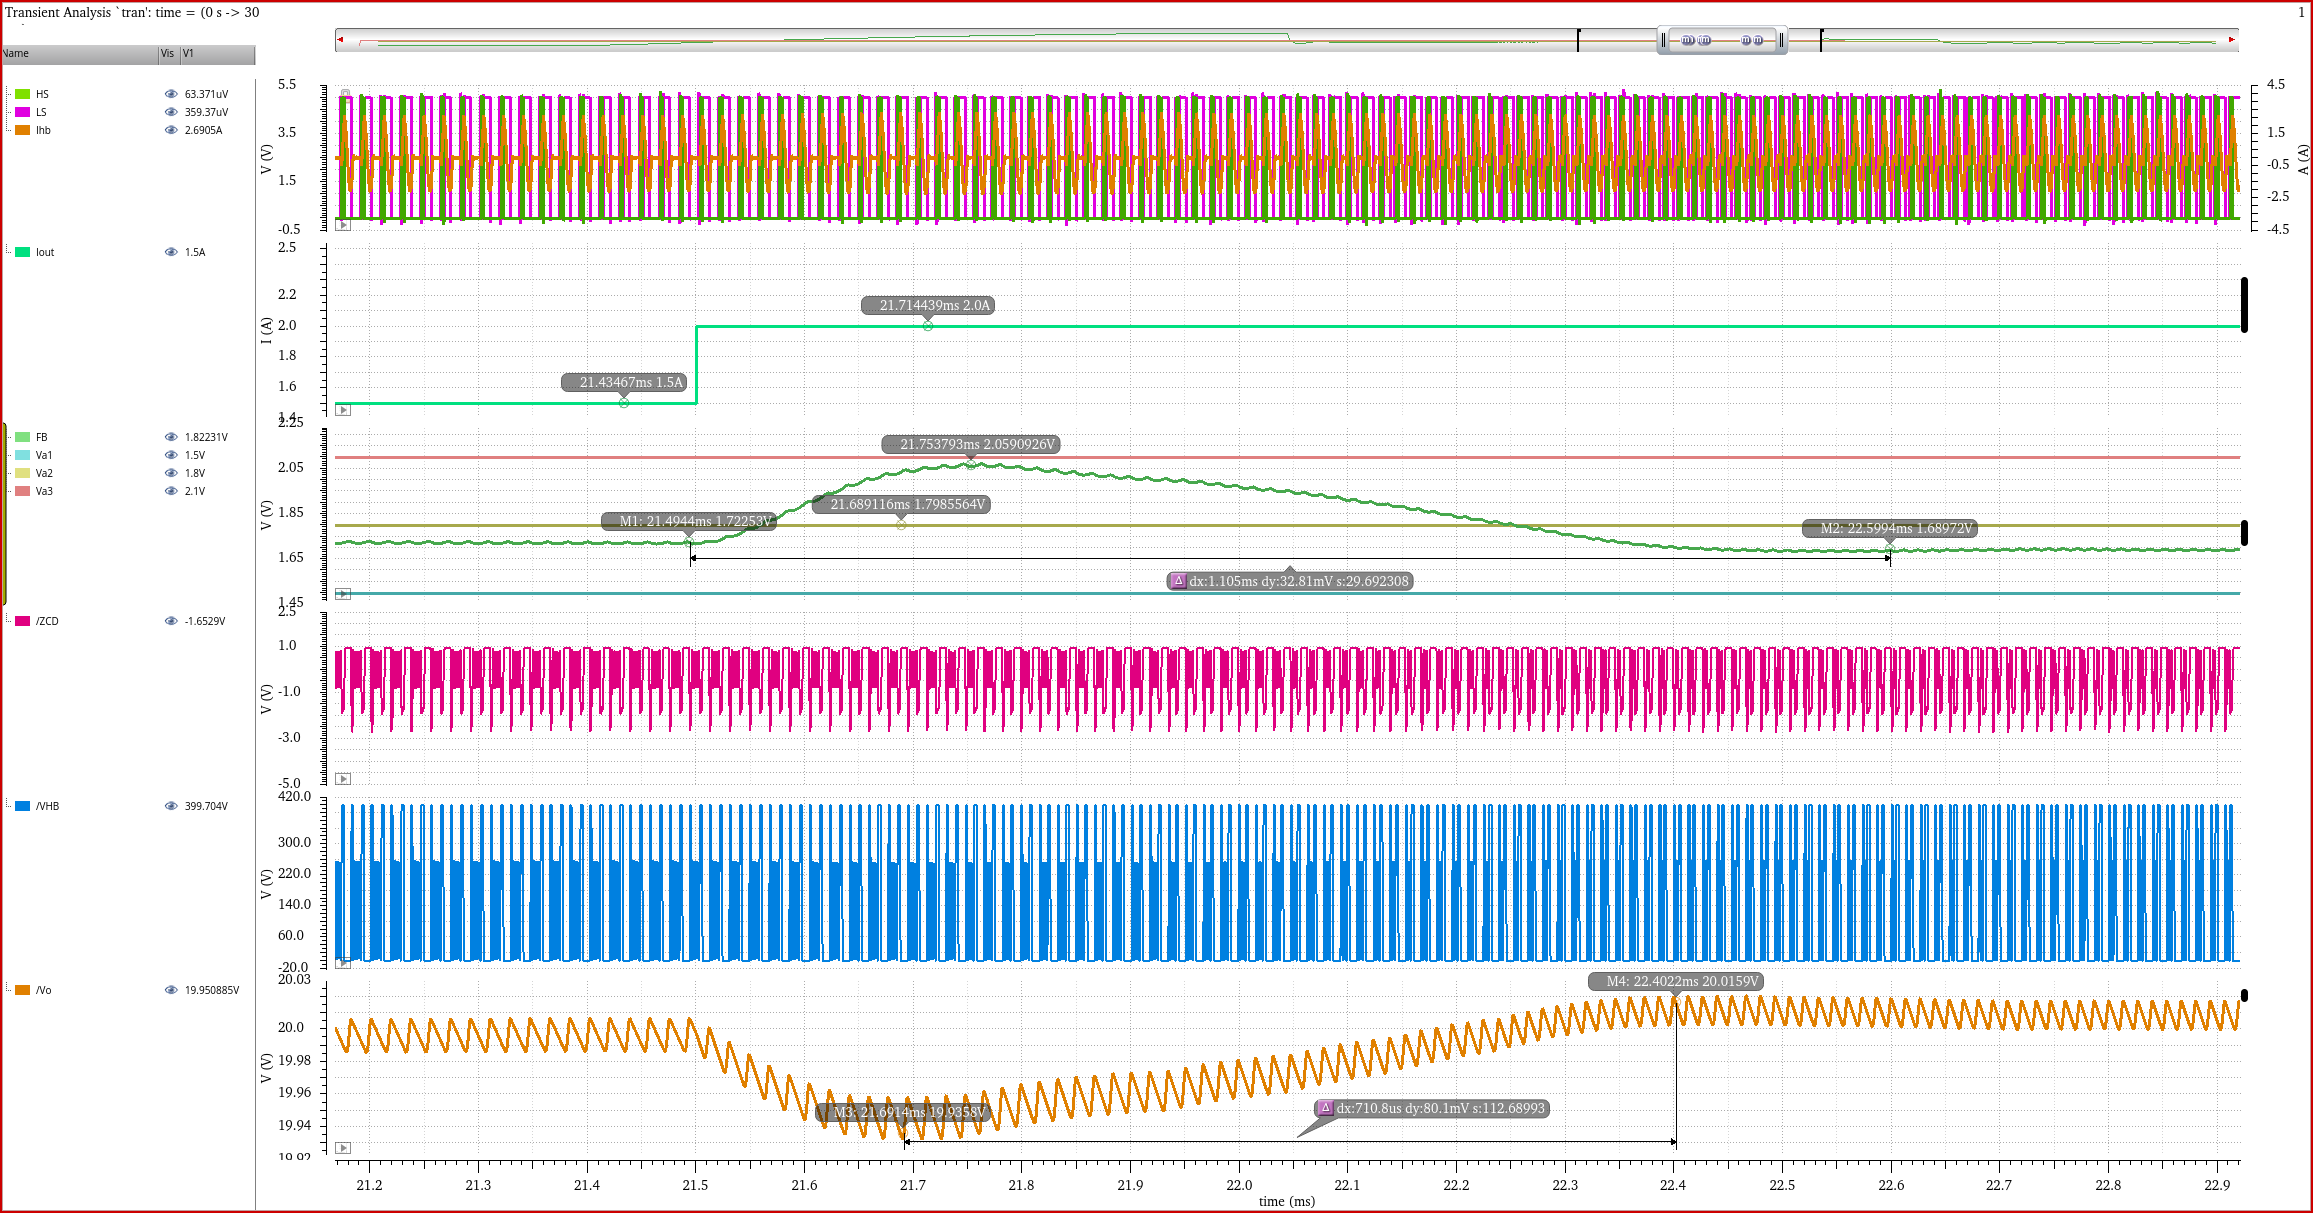
\includegraphics[width = 0.6\linewidth]{figures/valley_lock_slow.png}}
	\subcaptionbox{0A-2.5A  \label{fig:谷值锁定快切换仿真}}{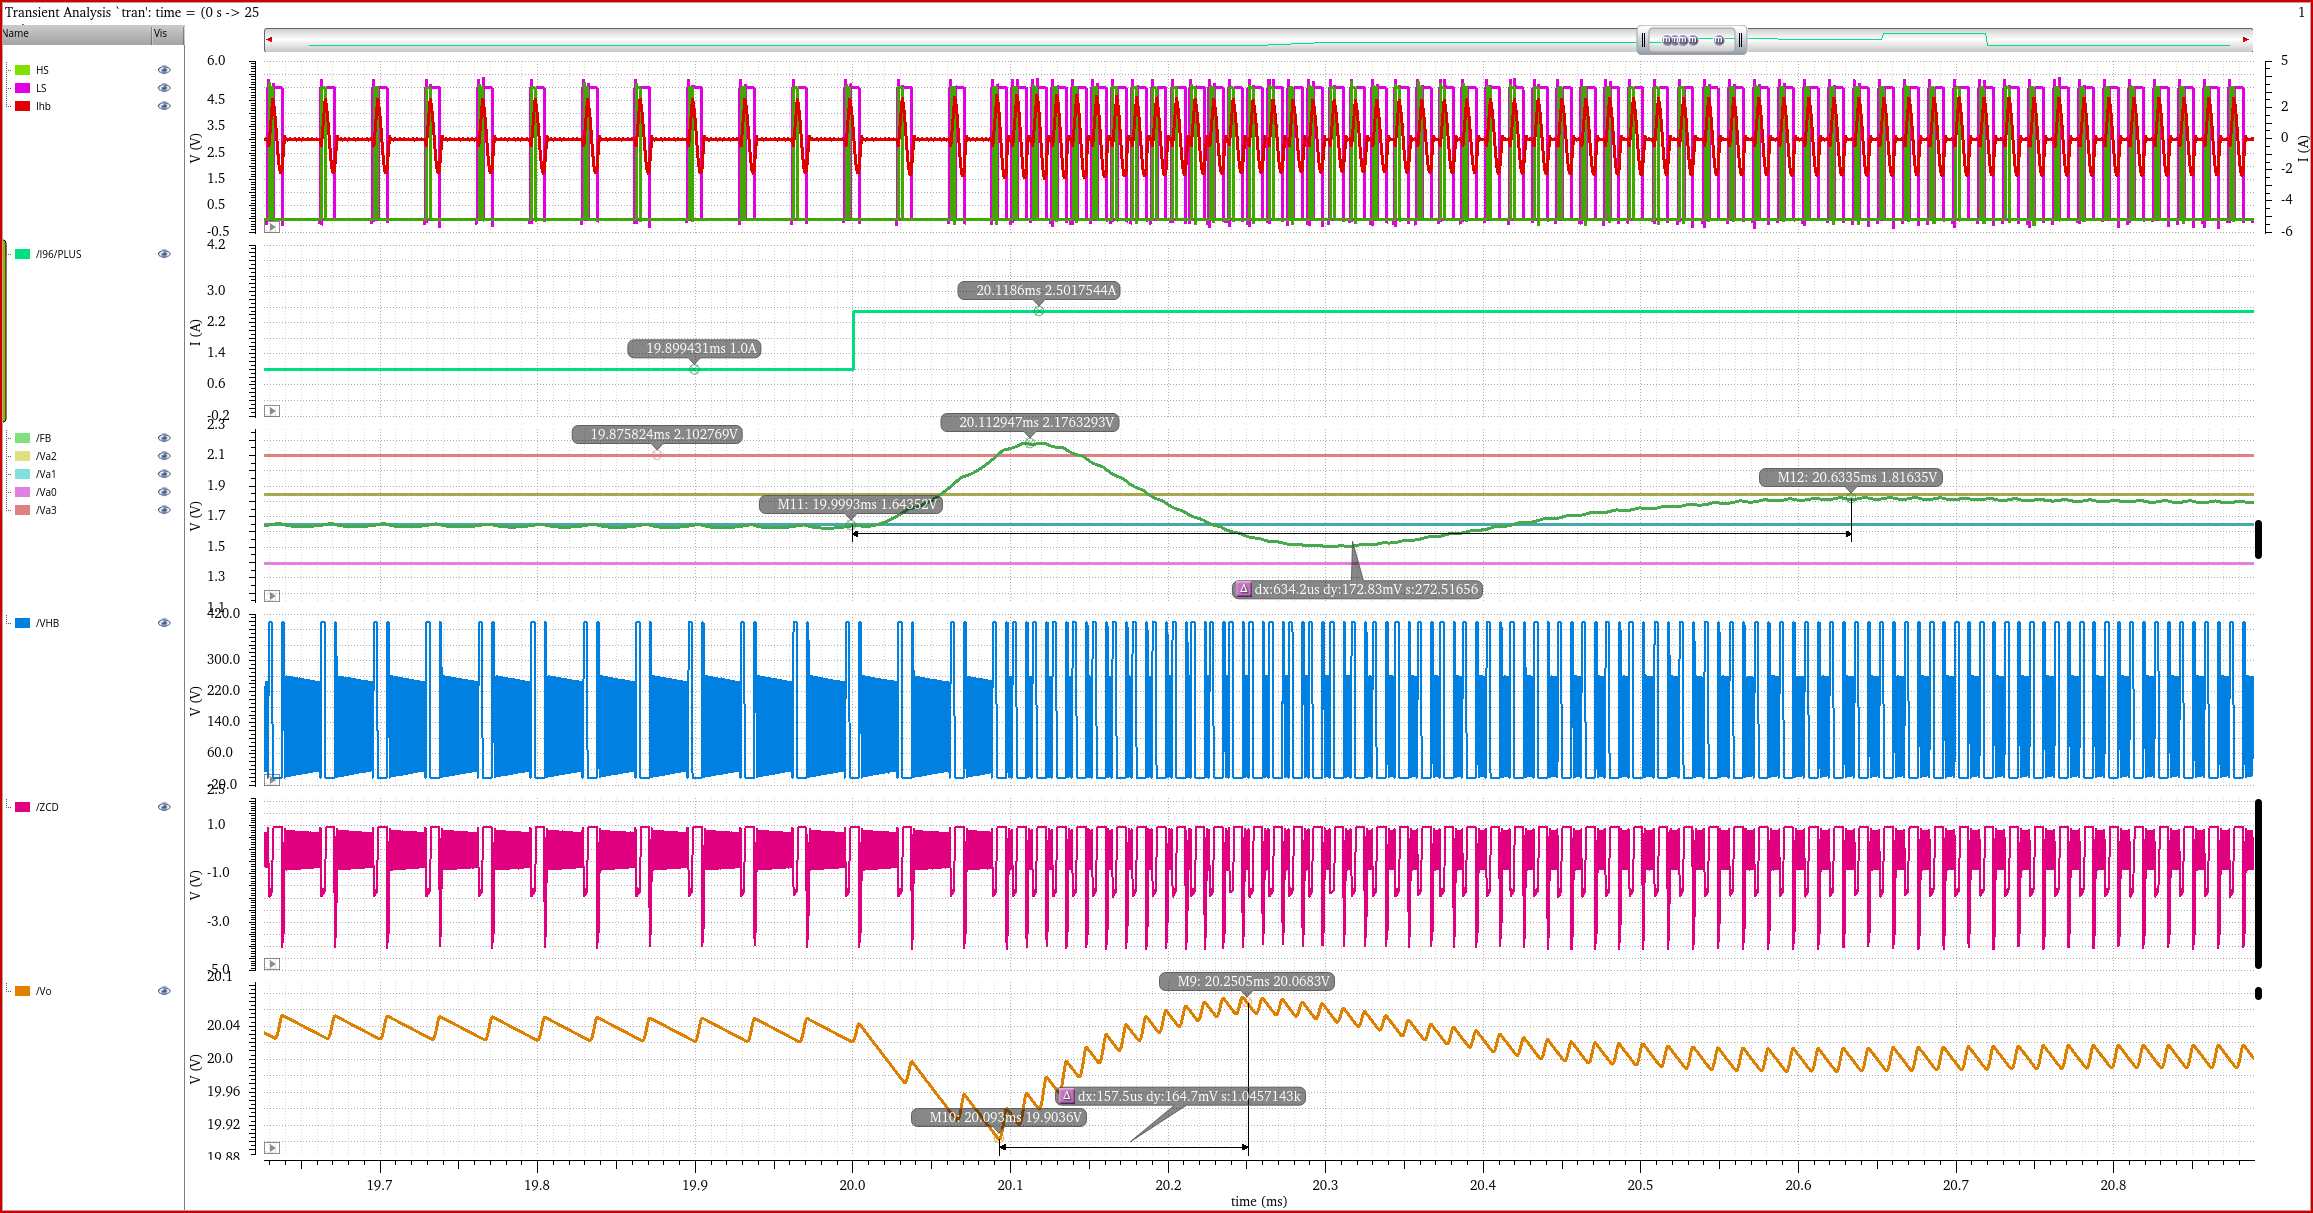
\includegraphics[width = 0.6\linewidth]{figures/valley_lock_fast.png}}
	\caption{快慢切换的谷值锁定仿真图}
	\label{fig:快慢切换的谷值锁定仿真图}
\end{figure}

其中图~\ref{fig:谷值锁定慢切换仿真}为负载电流小幅度地从1.5A变化为2A的仿真波形,$V_{FB}$未能大于参考电压$V_{a3}$,电路锁定的谷值数量逐次递减,直至$V_{FB}$小于参考电压$V_{a2}$直至稳定。可以观察到$V_{FB}$从发生变化到重新进入稳定区的时间共约为1.1ms,在$V_{FB}$的调制过程中输出电压$V_{o}$产生了约80mV的最大纹波,调制过程比较平稳,但响应速度略慢。

图~\ref{fig:谷值锁定慢切换仿真}为负载电流变化剧烈的仿真波形,从1A变化为2.5A,$V_{FB}$迅速大于参考电压$V_{a3}$,谷值锁定电路随机将谷值数量复位到了最小谷值数,直至$V_{FB}$在稳定区内稳定时,整个调制时间约为634us,调制过程中输出电压产生了约157mV的最大纹波。可以观察到,快切换策略减少了将近一半的响应时间,但由于谷值切换策略较为激进,导致输出电压的纹波略大。根据上文的全部仿真图,谷值锁定电路基本完成设计的功能,达成了预期的设计指标。


\section{退磁时间动态校准电路}

\subsection{退磁时间动态校准电路原理}

根据上文对~\ref{sec:退磁时间动态校准技术}小节中提到的退磁时间动态校准技术的分析,为了实现高效率的能量传递,应合理的调整低边功率管的导通时间,力求让导通时间和励磁电感的退磁完成时间尽可能的接近。

退磁完成时间会受到多方面因素的影响,如输出电压、输出负载电流、原边峰值电流大小和芯片外围变压器漏感、谐振电容等器件。难以通过计算直接求得退磁完成时间,常规的退磁时间设定技术是通过将退磁时间和输出电压联系起来,采用开环电路控制低边功率管的导通时间。但当输出负载发生波动或外围器件采用不同参数配置时,开环的电路无法对每种情况都匹配,实现最大的能量传递。故本文通过如图~\ref{fig:退磁时间1}中所示的退磁时间动态校准技术完成闭环设计,实现最高的能量传递效率。

\begin{figure}[htbp] 
    \centering
    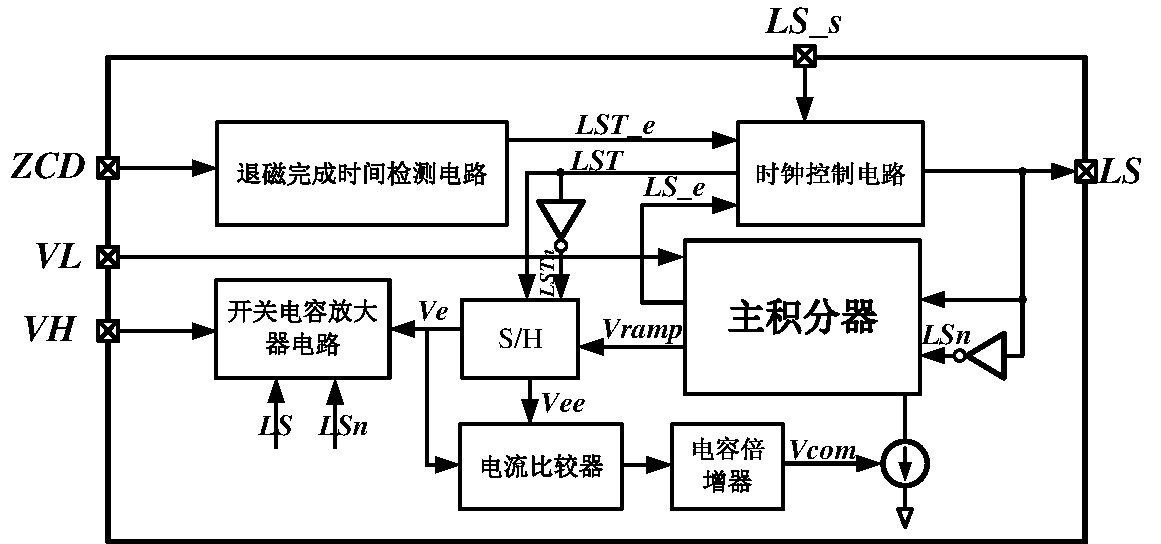
\includegraphics[width=0.8\linewidth]{figures/退磁技术框图.pdf}
    \caption{退磁时间动态校准电路框图}
    \label{fig:退磁时间动态校准电路框图}
\end{figure} 

图~\ref{fig:退磁时间动态校准电路框图}中所示为退磁时间动态校准电路的主要模块框图,主要包括退磁完成时间检测、时钟控制、主积分器、开关电容放大器、电流比较器和电容倍增器等电路。该电路方案通过退磁完成时间检测电路采样得到ZCD引脚电压信号$V_{ZCD}$上的高频谐振信号,输出退磁完成时间结束信号LST\_e,在该信号产生时刻原边电流和漏感电流相交,能量传递结束。但为了防止输出负载微小波动引起的信号LST\_e不稳定情况,不能直接用该信号直接控制低边功率管关断,导致其导通时间的不稳定问题,而是通过动态校准技术延缓变化速度,逐周期逼近到最新的退磁完成时间。

\begin{figure}[htbp] 
    \centering
    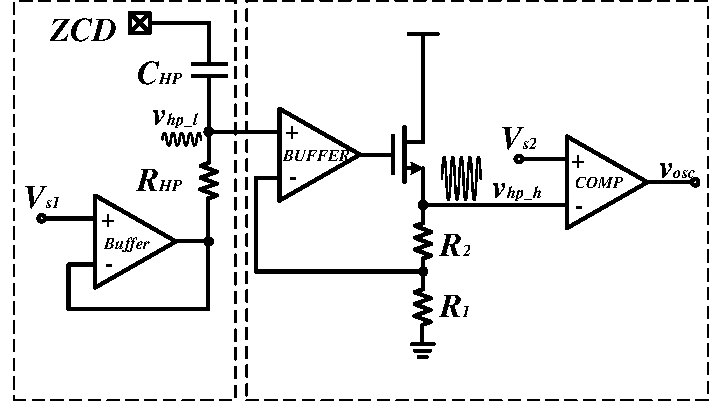
\includegraphics[width=0.6\linewidth]{figures/退磁时间检测电路.pdf}
    \caption{退磁完成时间检测电路}
    \label{fig:退磁时间检测电路}
\end{figure} 

退磁完成时间检测电路的如图~\ref{fig:退磁时间检测电路}中所示,包括高通滤波电路和小信号放大电路,高通滤波电路输入端连接$V_{ZCD}$电压信号,高通滤波模块由$C_{HP}$和$R_{HP}$组成,用于将$V_{ZCD}$电压信号上的微小高频谐振信号采样到给定电压$V_{s1}$上得到电压信号$V_{hp,l}$,再经过弱信号放大模块放大后得到电压信号$V_{hp,h}$,$V_{hp,h}$与给定电压$V_{s2}$通过比较器进行比较,得到输出的退磁完成时间结束信号LST\_e,触发时钟控制电路生成控制信号LST。信号LST不能直接用于控制低边功率管,后续通过图~\ref{fig:退磁时间动态校准电路框图}中其他电路组成的动态校准闭环补偿结构产生功率管实际关断信号LS\_e,通过时钟控制电路生成逻辑控制信号LS去控制低边功率管的导通时间。

\begin{figure}[htbp] 
    \centering
    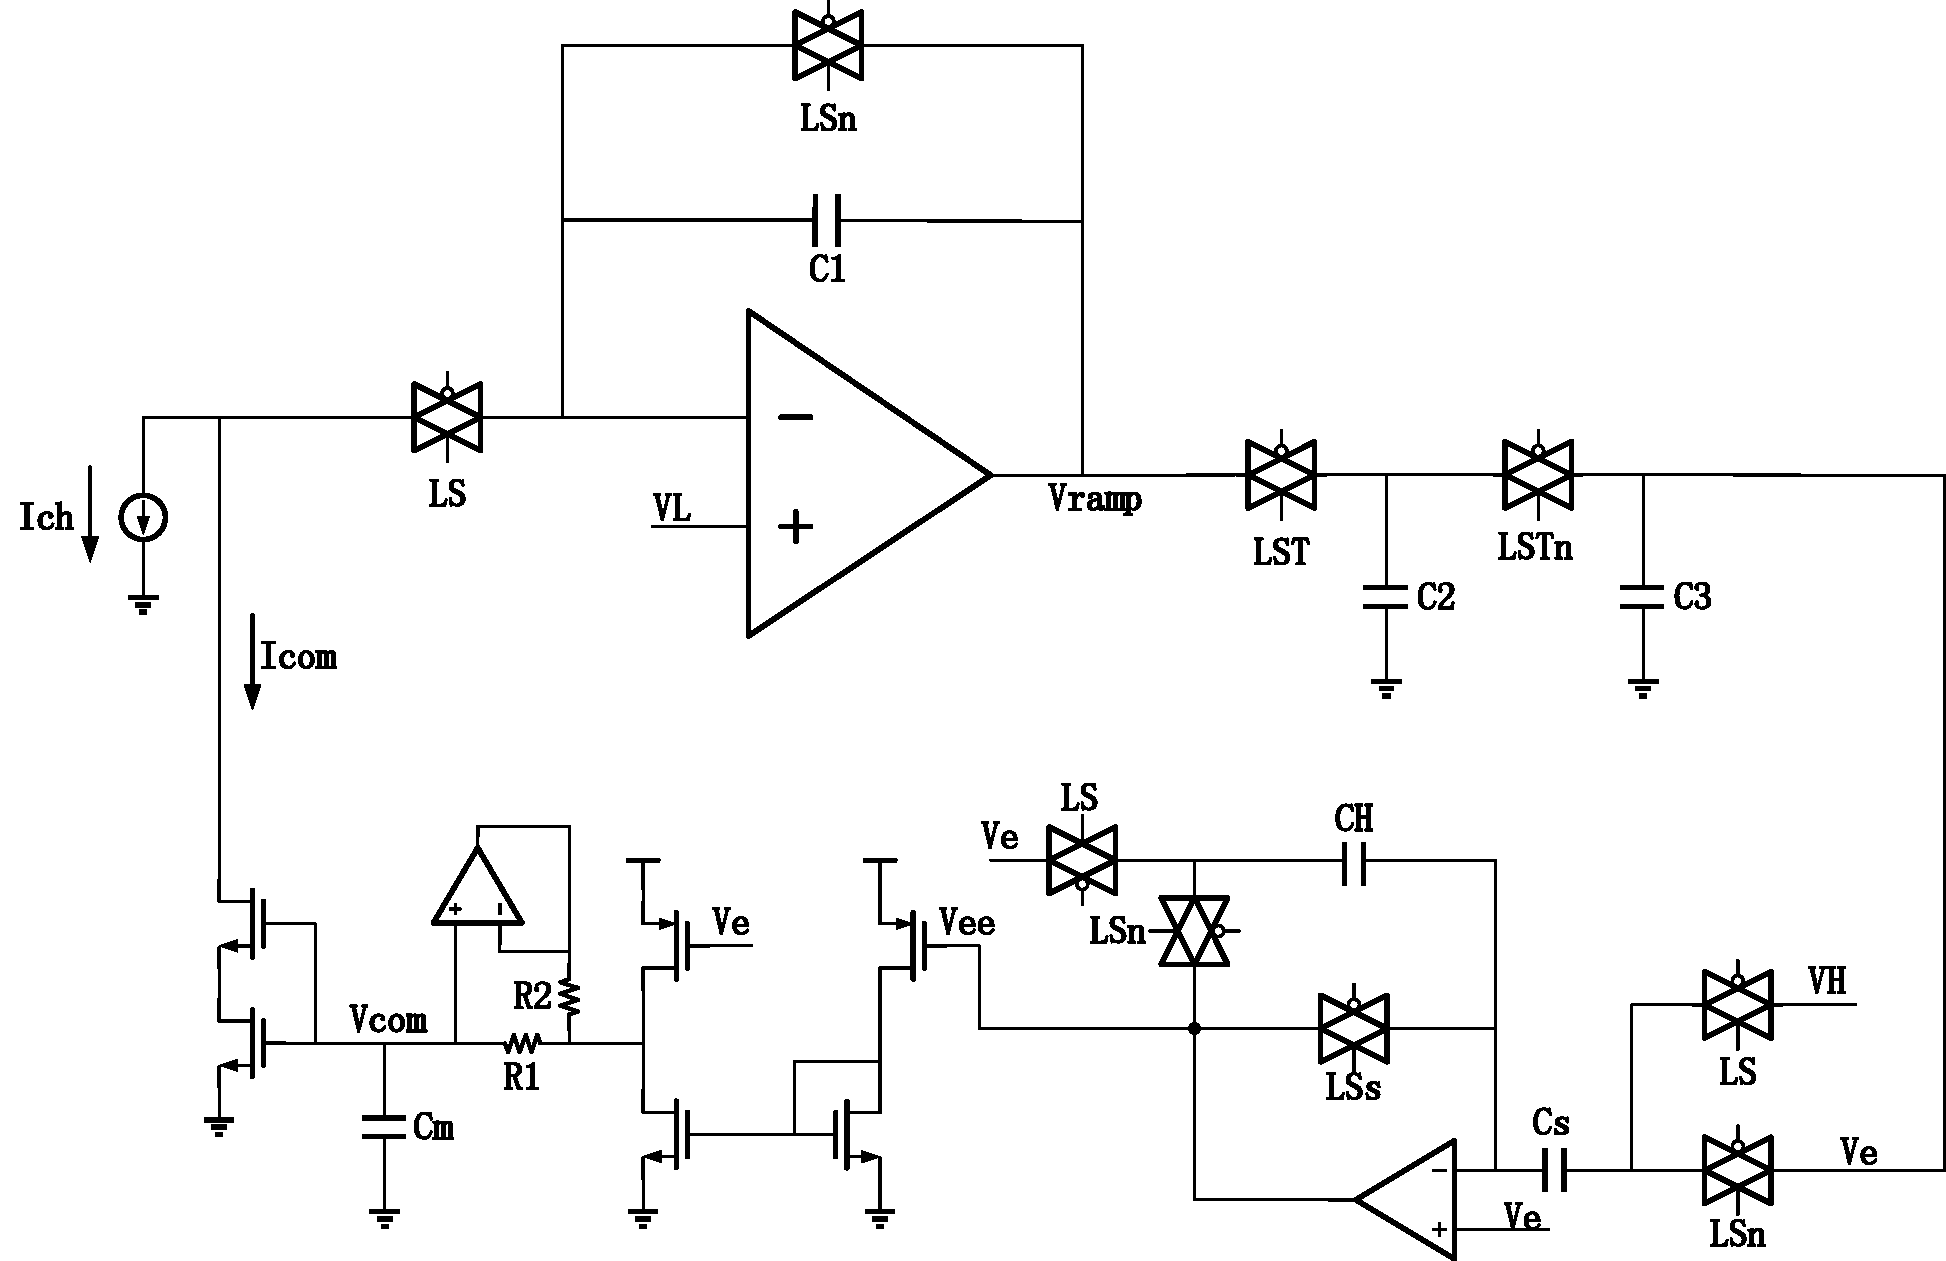
\includegraphics[width=0.8\linewidth]{figures/主积分器环路电路.pdf}
    \caption{动态校准闭环补偿电路}
    \label{fig:动态校准闭环补偿电路}
\end{figure} 

\begin{figure}[htbp] 
    \centering
    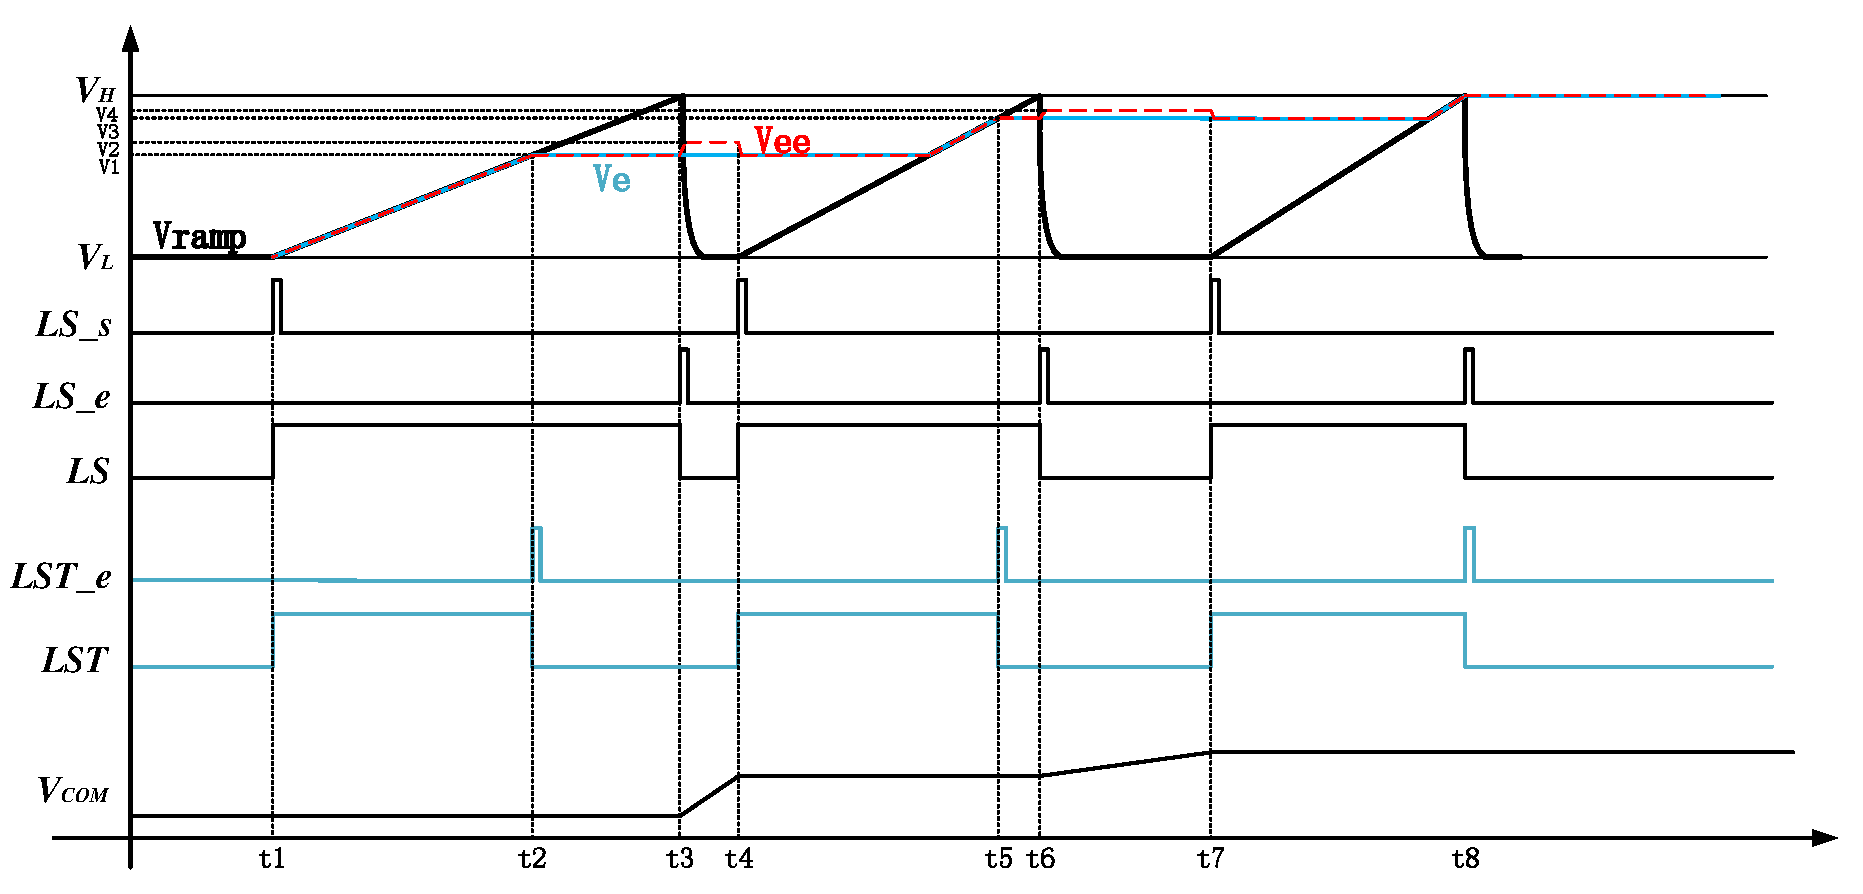
\includegraphics[width=0.8\linewidth]{figures/主积分器环路波形图.pdf}
    \caption{动态校准闭环补偿波形示意图}
    \label{fig:动态校准闭环补偿波形图}
\end{figure} 

图~\ref{fig:动态校准闭环补偿电路}和~\ref{fig:动态校准闭环补偿波形图}分别是动态校准闭环补偿结构的电路图和波形图。该结构的具体工作过程为:

在t1时刻外部输入脉冲信号LS\_s由低电平转为高电平,时钟控制模块输出的时钟信号LS和LST被LS\_s信号触发同样由低电平转为高电平,LS信号开始控制电流Ich对主积分器的积分电容进行充电,输出斜率为k1积分斜坡电压$V_{ramp}$,LST信号控制采样保持电路采样电压信号$V_{ramp}$。

电路经过一段时间到达t2时刻,高通滤波采样放大电路检测到外部输入电压信号$V_{ZCD}$的高频谐波振荡,产生脉冲信号LS\_e使得时钟控制电路将时钟信号LST由高电平拉低到低电平,进而将采样电压Ve保持在固定的电压V1处。

在LS为高电平的时间阶段内,开关电容电路同时工作在采样阶段,使得输出电压Vee一直等于前级输入电压Ve,因此后级的电流比较器电路两个PMOS晶体管栅极电压保持相等,Ie和Iee近似相同,没有多余的电流对后级的大电容进行充放电,电容电压$V_{com}$维持不变,由NMOS构成的VCCS也不产生补偿电流Icom改变主积分器电路输出积分斜坡电压$V_{ramp}$的斜率。

直至电路工作到t3时刻,主积分器积分斜坡电压$V_{ramp}$大于给定固定电压VH,产生脉冲LS\_e使得时钟控制电路控制时钟信号LS由高电平拉低为低电平,开关电容放大器电路改变为保持放大模式,将输出电压Vee放大到固定电压V2处;此时开关电容放大器电路输出电压Vee大于采样保持电压Ve,电流比较器输出的电流Ie大于Iee,开始为后级电容倍增电路产生的大电容进行充电,电压$V_{com}$逐渐增大,经过VCCS后产生的补偿电流也Icom逐渐增大。

电路继续工作到t4时刻,外部输入的脉冲信号LS\_s再次由低变高,电路进入下一周期,由于上一周期产生的补偿电流Icom增大到一定值,因此本周期主积分器输出的积分斜坡电压$V_{ramp}$的斜率增大到k2,由于斜率增大,斜坡电压$V_{ramp}$将更快的大于给定固定电压VH,使得时钟控制电路产生的时钟信号LS相较于前一周期更短,更接近时钟信号LST的脉宽长度。

电路经过与前一周期同样的工作流程后,电压信号$V_{com}$再次在LS信号为低电平时逐渐增大,补偿电流Icom也相应增大,进而控制下一周期的积分斜坡电压$V_{ramp}$继续增大,时钟信号LS进一步缩短,逐步逼近时钟信号LST。

\subsection{退磁时间动态校准电路仿真分析}


\begin{figure}[htbp] 
    \centering
    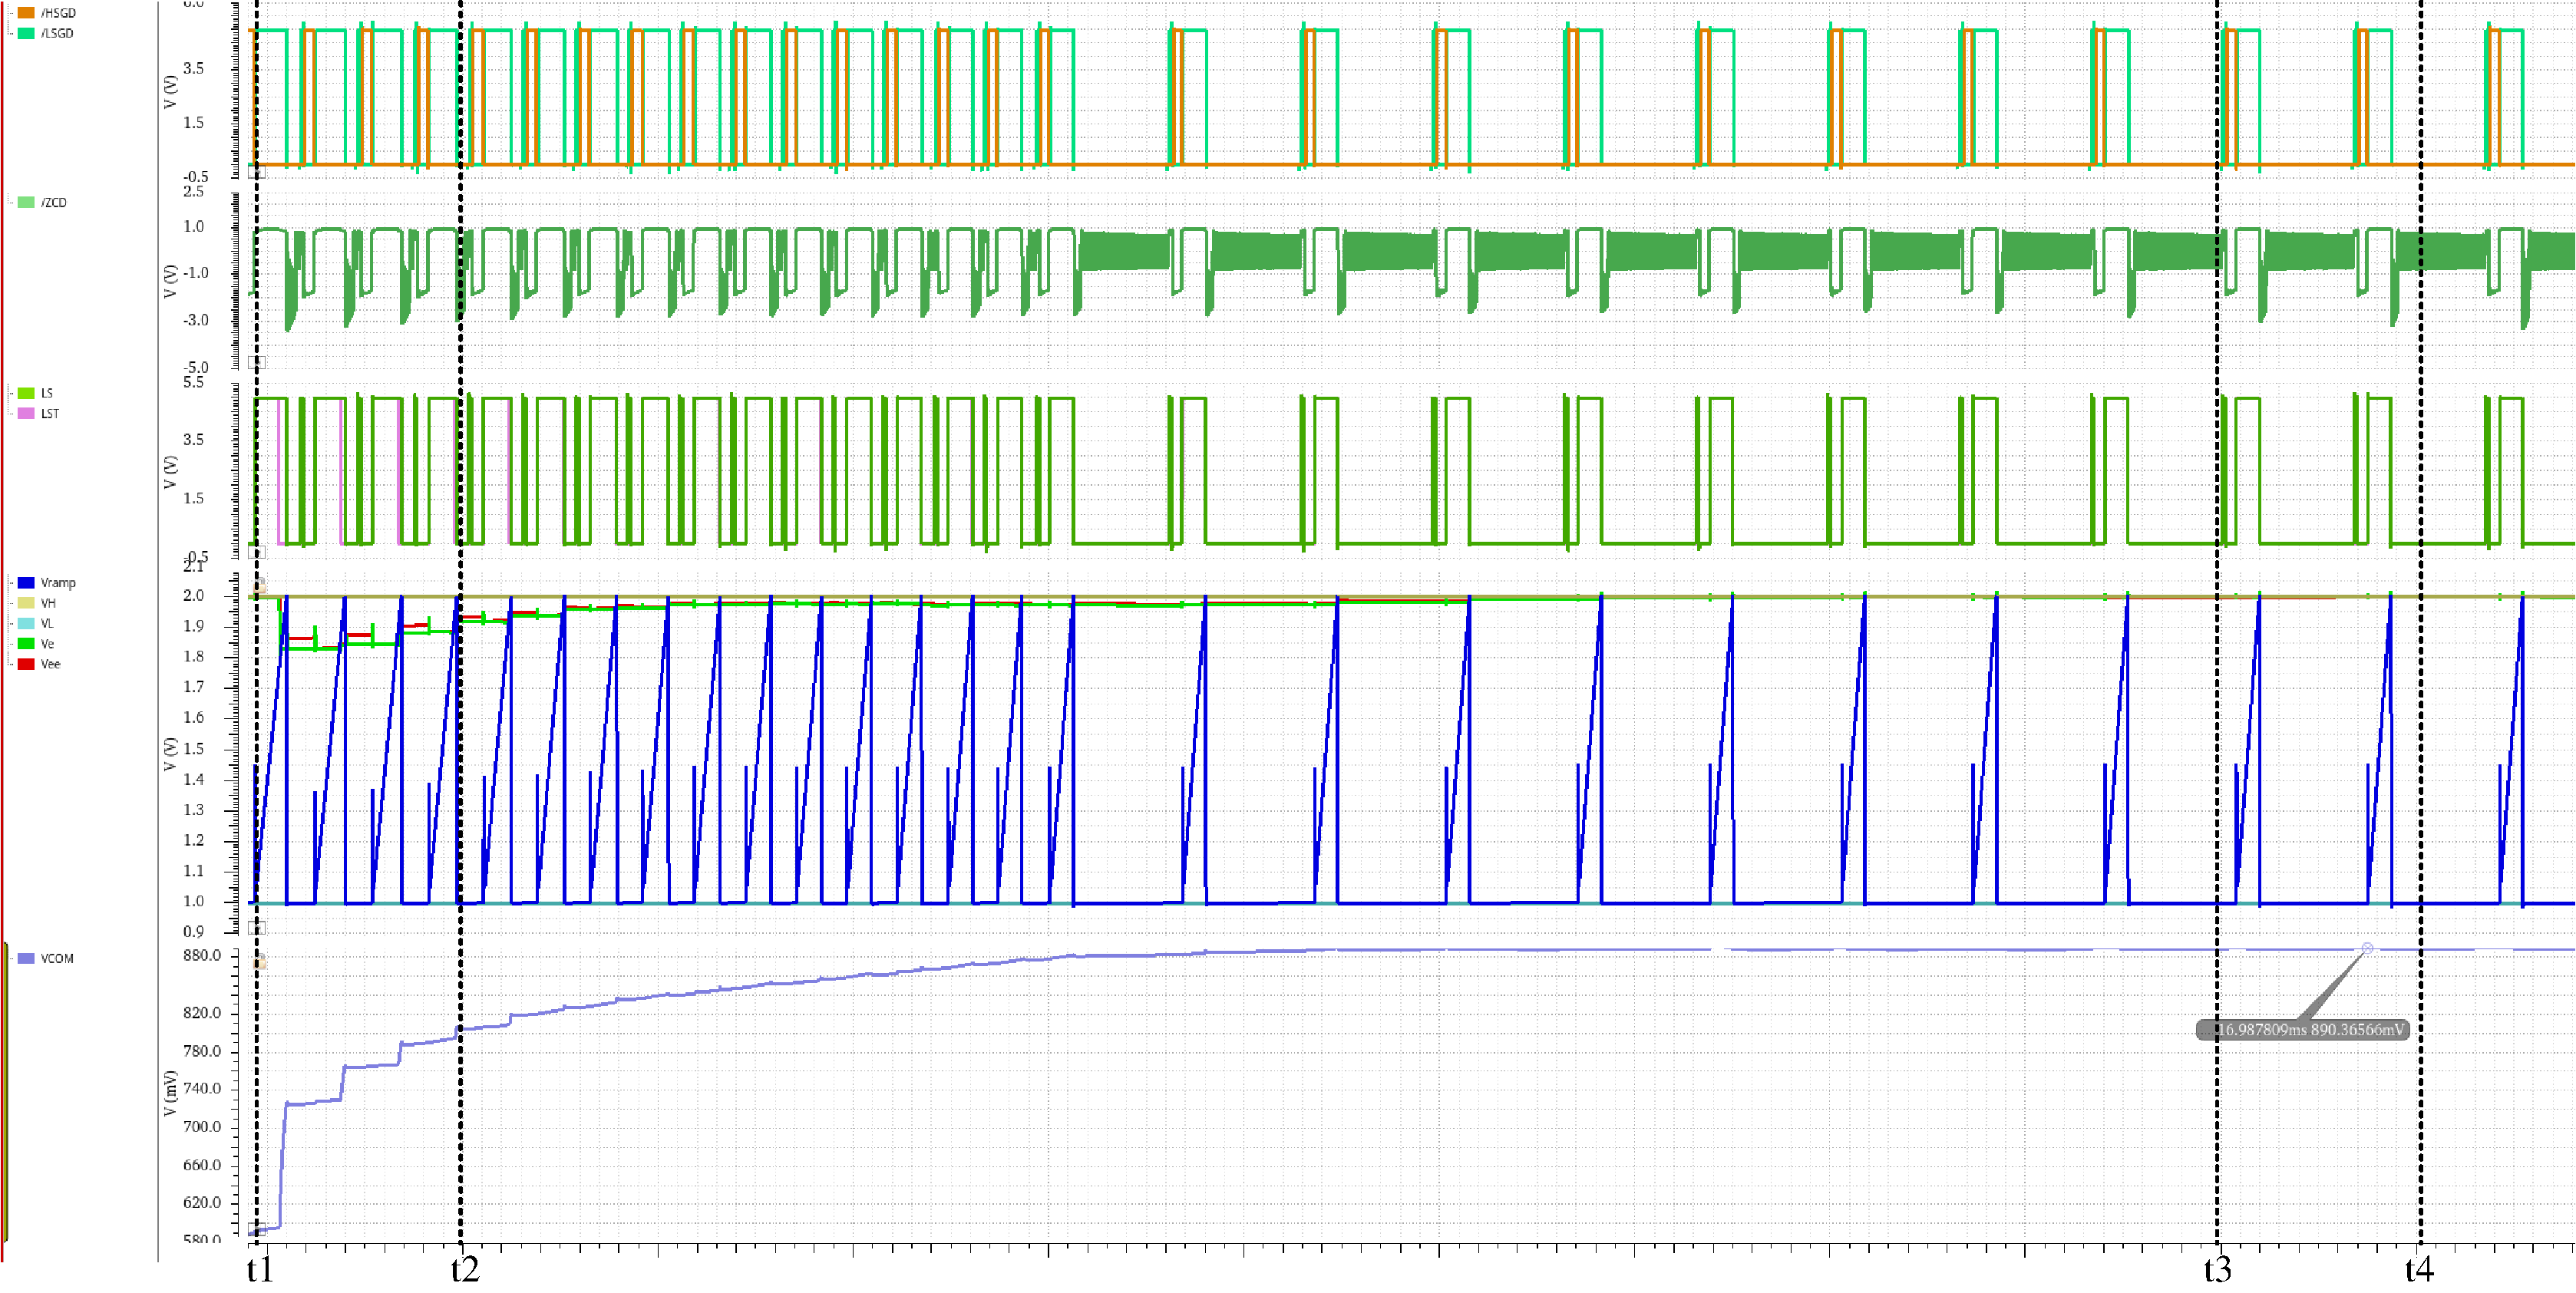
\includegraphics[width=0.9\linewidth]{figures/StepByStep.pdf}
    \subcaptionbox{未稳定\label{fig:退磁时间仿真图1}}{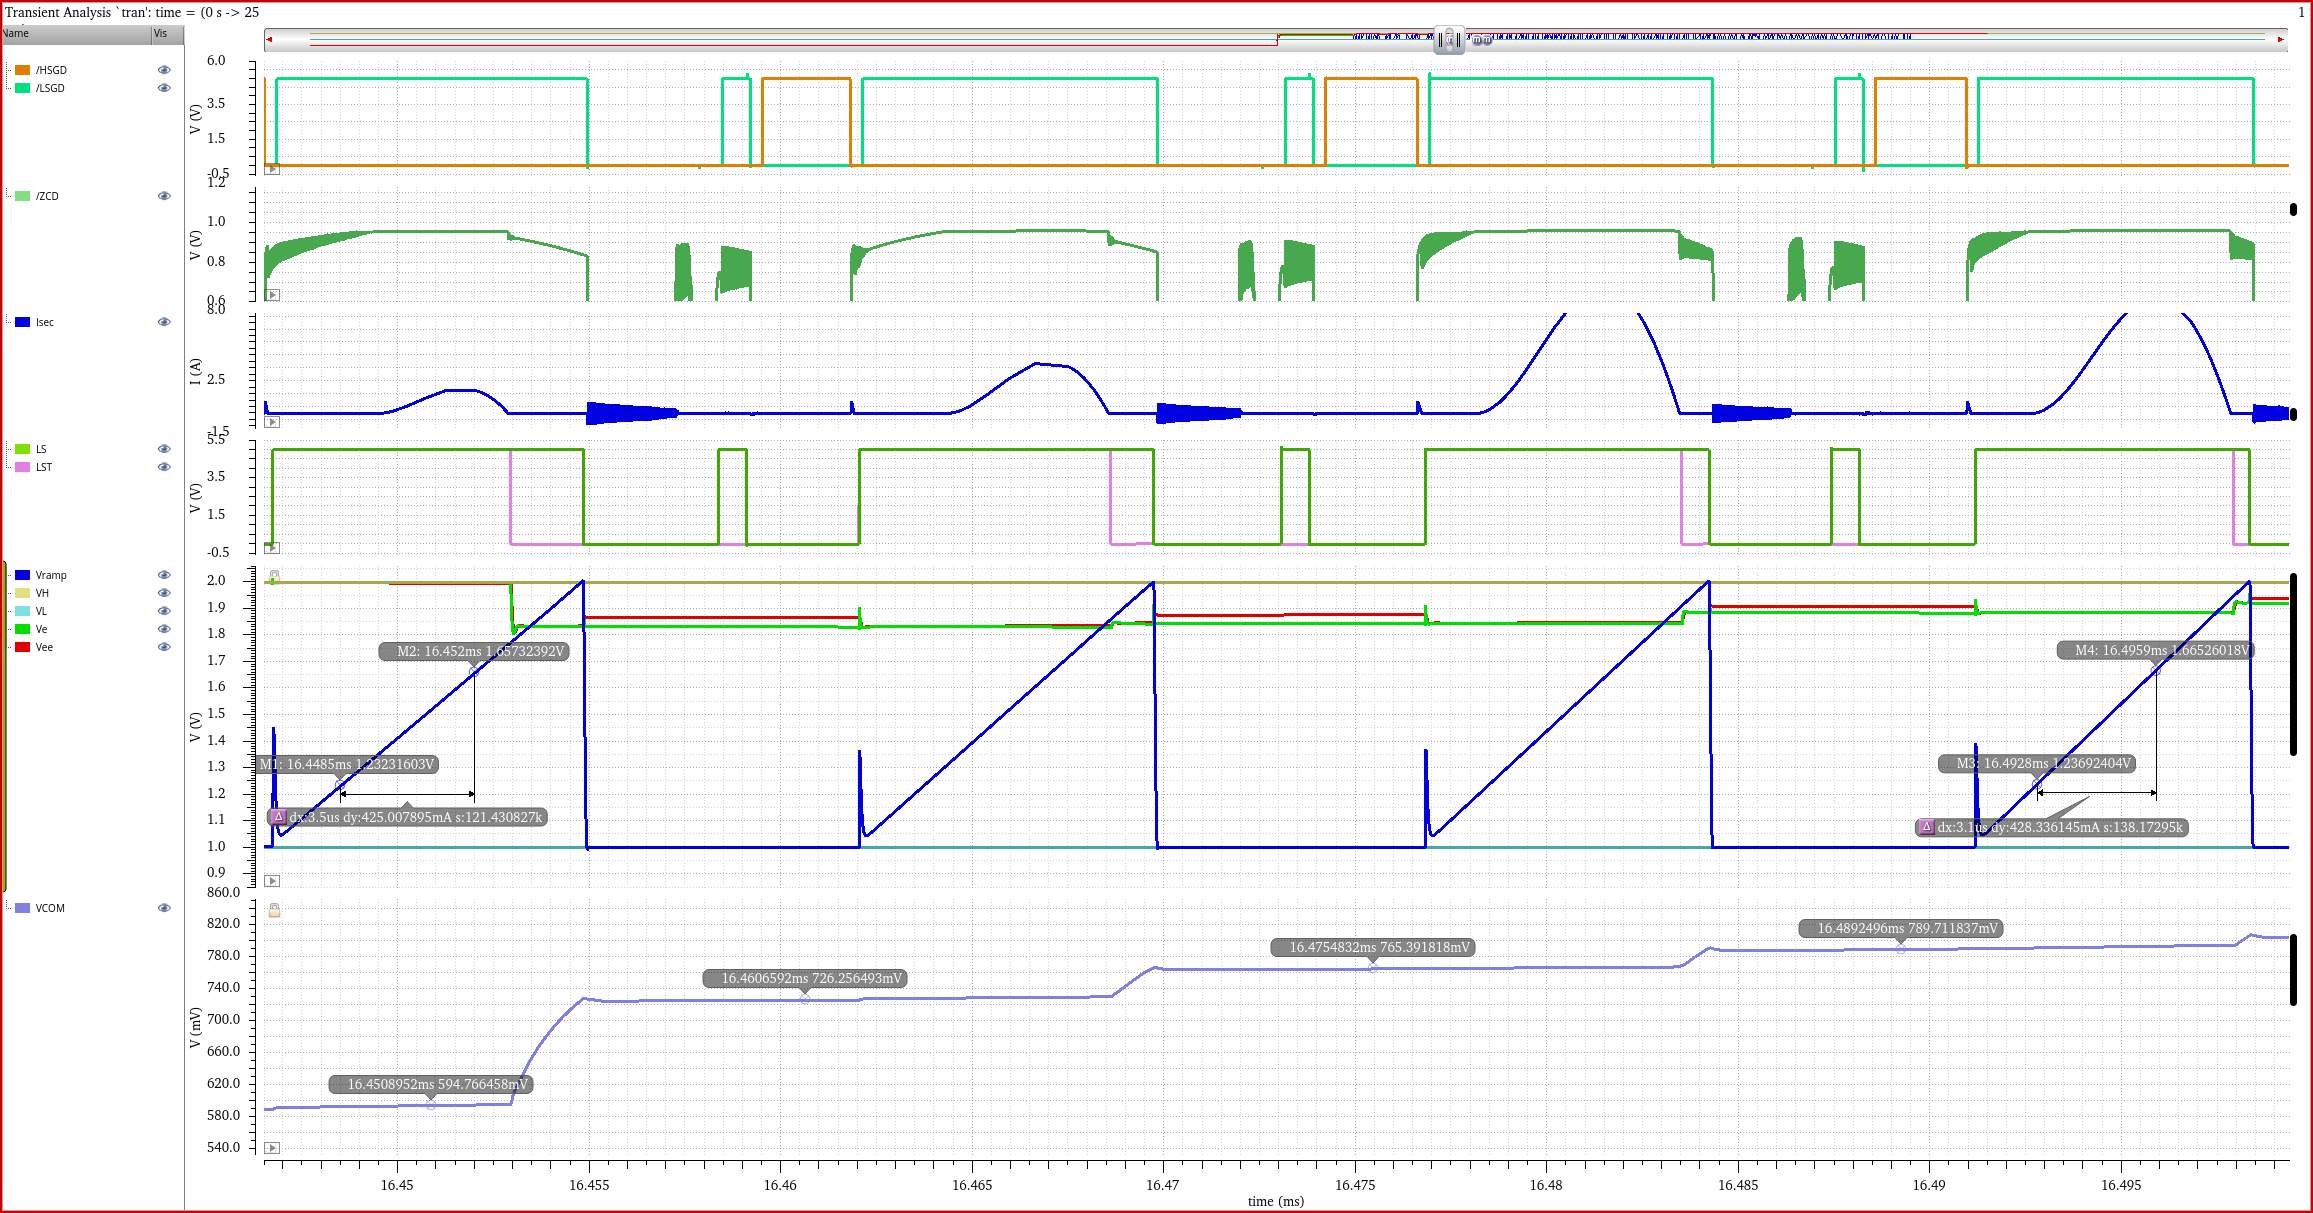
\includegraphics[width = 0.6\linewidth]{figures/stepbystep1.png}}
	\subcaptionbox{稳定  \label{fig:退磁时间仿真图2}}{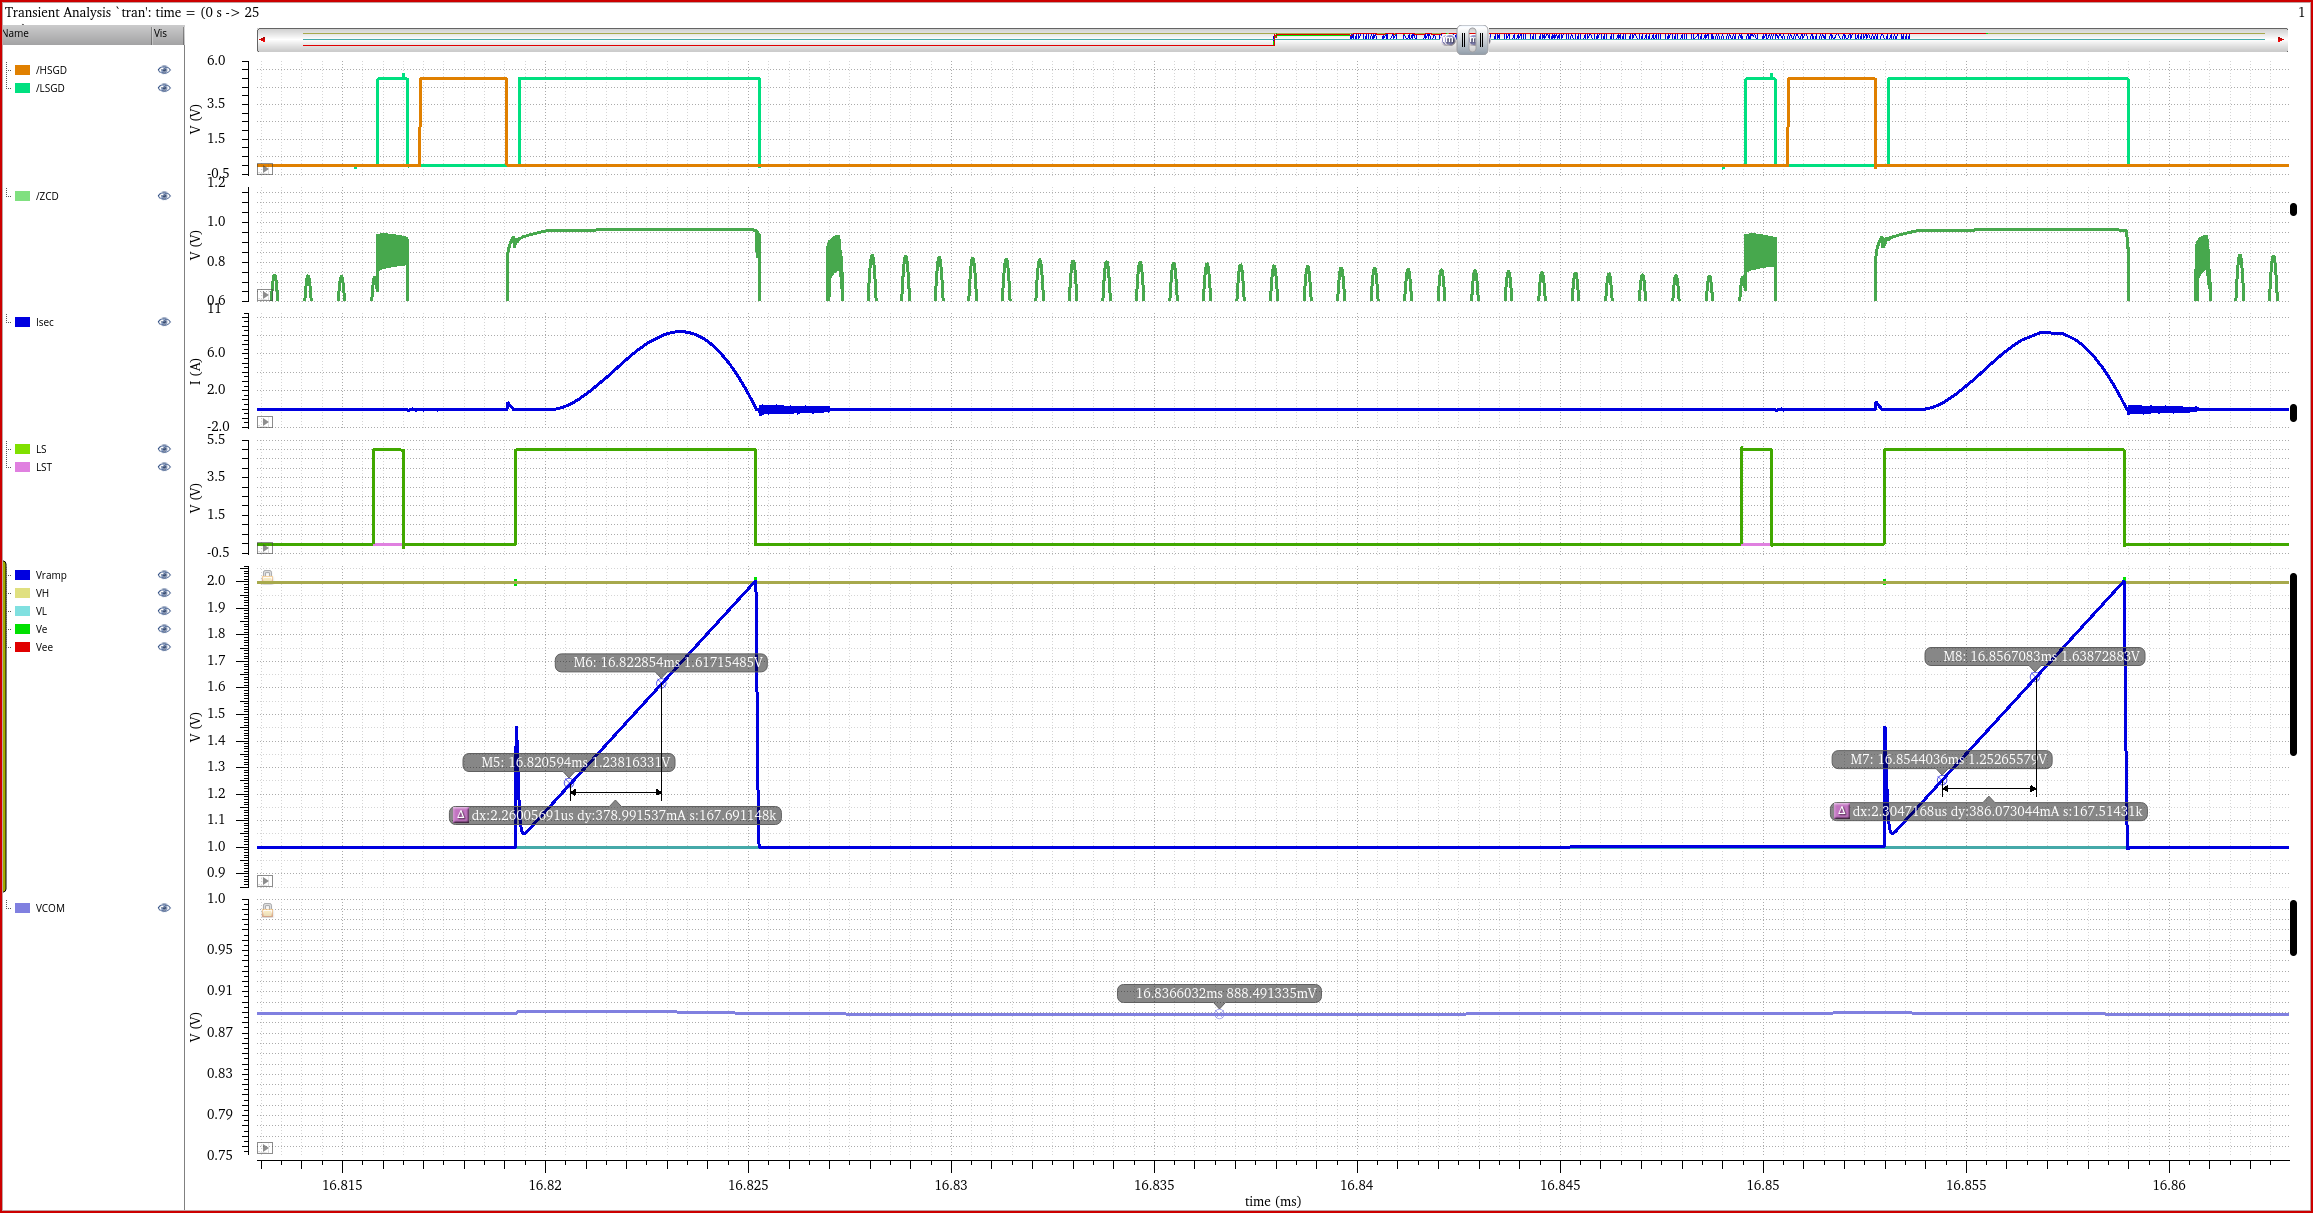
\includegraphics[width = 0.6\linewidth]{figures/stepbystep2.png}}
    \caption{退磁时间动态校准电路波形图}
    \label{fig:退磁时间动态校准电路波形图}
\end{figure}

退磁时间动态校准电路的具体波形图如图~\ref{fig:退磁时间动态校准电路波形图}所示,该波形图和图~\ref{fig:动态校准闭环补偿波形图}中的示意波形一致,从具体的仿真波形图可以看到,在$t_1$时刻所处的开关周期内,逻辑控制信号LS未能和退磁完成时间信号LST重叠,说明此时低边功率管的导通时间较长,能量虽完全传递到副边但变压器未立刻反转导致的原边电流反向励磁产生了很多不必要的损耗,但随着通过几个开关周期的不断逼近,在$t_4$时刻补偿电压$V_{com}$逐渐稳定在888mV处,电压Vee和Ve也都贴近了参考电压VH,逻辑控制信号LS和励磁电感退磁完全时间信号LST重叠,此时低边功率管导通时间近似完全等于原边励磁电感退磁完成时间,实现了能量的最大传递功能。其中,由于输出负载电流突变引起的开关频率变化也未对退磁时间动态校准电路的结果产生影响,证明了该电路在不同负载下的兼容性。

图~\ref{fig:退磁时间仿真图1}为整体仿真图中斜坡电压$V_ramp$未稳定时,$t_1$到$t_2$时间段内的四个开关周期的仿真图,可以观察到第一个开关周期内信号$V_{ZCD}$上的高频谐波振荡,在此高频振荡处,副边电流$I_{sec}$刚好降低为零,原副边的能量传递结束,信号LST从高电平降低为低电平,此时积分器斜坡电压$V_ramp$的斜率较低,等于121kV/s,补偿电压在信号LS和信号LST未重叠区间内逐渐增大,提高积分器斜坡电压的$V_ramp$的下一周期斜率,在该图中的第四个开关周期斜坡斜率已增大为138kV/s,信号LS和信号LST未重叠区间也大大减小,逐步逼近功能实现优异。图~\ref{fig:退磁时间仿真图2}为斜坡电压$V_ramp$稳定时,$t_3$到$t_4$时间段内两个开关周期的仿真图,可以观察到此时补偿电压$V_{com}$不在发生变化,两个开关周期内斜坡电压$V_ramp$的斜率也同时维持在167kV/s,证明了该退磁时间动态校准电路的基本功能已实现,充分提高了整体系统的高效率能量传递且具有较好的鲁棒性。












\section{逻辑控制电路}

逻辑控制电路是用于控制片外功率管导通和关断的关键电路,通过电路内各种数字逻辑接收、综合和处理变换器芯片内的其他模块的各种指示信号,最终输出高低边功率管的逻辑控制信号HS和LS给驱动电路。

\subsection{逻辑控制电路原理}

由于本文介绍的非对称半桥反激式变换器采用了不同负载下的多模式控制,尤其是RVS工作模式和CRM工作模式的切换过程中,不仅发生了开关周期长短的变化,还需要改变对高低边功率管的导通和关断顺序;同时不论是RVS工作模式在精确谷底导通模块的要求或是CRM工作模式的最大能量传递要求,都导致了变换器芯片内不能使用恒定的时钟信号对开关周期的开启进行控制,涉及到不同负载不同工况下开关周期开启信号的变化,这些都加大了逻辑控制电路的设计难度。

\begin{figure}[htbp] 
    \centering
    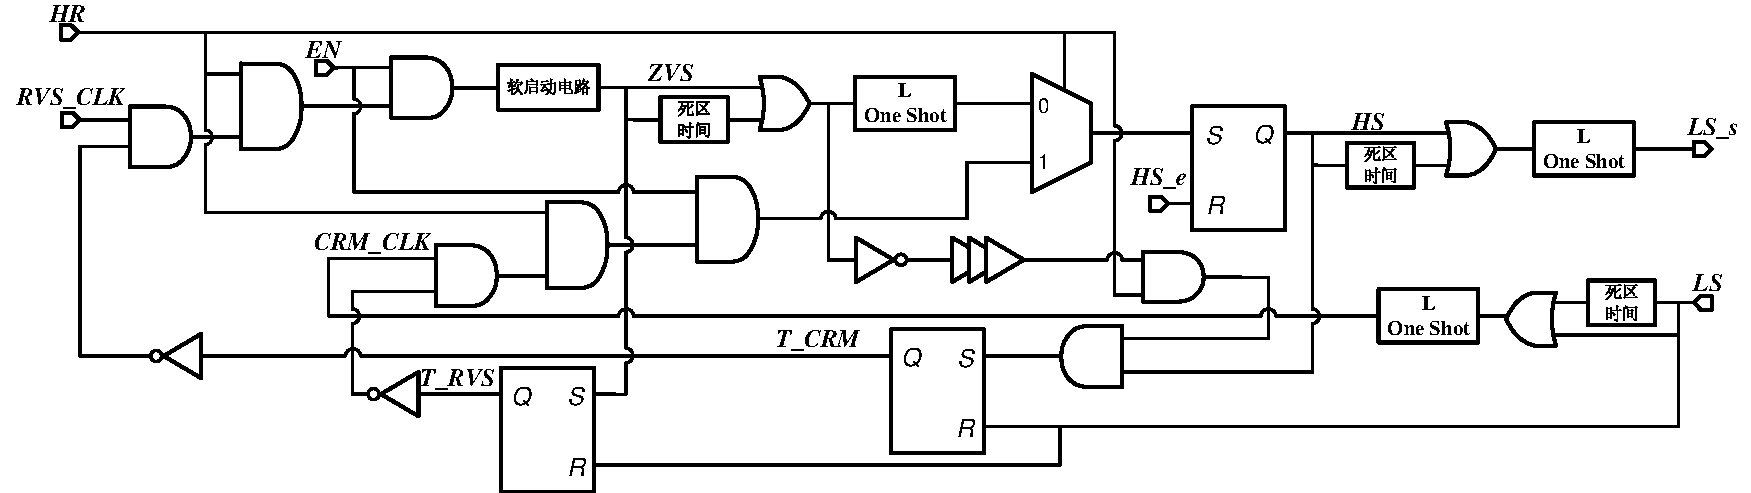
\includegraphics[width=1.0\linewidth]{figures/逻辑控制电路.pdf}
    \caption{逻辑控制电路原理图}
    \label{fig:逻辑控制电路原理图}
\end{figure} 

逻辑控制电路的具体原理图如图~\ref{fig:逻辑控制电路原理图}所示,包含多个输入输出信号,其中信号EN是变换器芯片的整体使能信号;信号HR表征输出负载轻重程度,决定了电路的具体工作模式,当信号HR为逻辑“1”时,此时负载电流较大,电路应工作在CRM模式,信号HR为逻辑“0”时,电路工作在RVS模式;信号RVS\_CLK是如图~\ref{fig:精确谷底导通技术框图}中所示的精确谷底导通模块输出的时钟信号;信号HS\_e是电感电流采样电压和峰值电流电压通过比较器输出的信号,控制着低边功率管的关断;信号LS\_s是输出给退磁时间动态校准电路的控制信号,控制着逻辑控制信号LS的上升沿的产生;同时退磁时间动态校准电路将产生的信号LST输入到逻辑控制电路中用于后续的控制。

电路通过使用一个MUX选择器根据信号HR的高低电平选通逻辑SR锁存器1的S输入端后产生逻辑控制信号HS。

在不考虑SR锁存器2和3的输出,当信号HR为低电平时,系统应工作在RVS模式,输入的谷底时钟信号RVS\_CLK经过一些与门后输入到软启动时间电路中产生信号ZVS,信号ZVS输入到死区时间电路中产生功率管全部关闭的死区时间信号,两个信号再通过或门相或后经过一个下降沿脉冲电路输入到SR锁存器1的S端,并和R端的信号HS\_e一起产生逻辑控制信号HS。信号HS再次和死区时间电路的输出信号相或后经过脉冲电路产生控制信号LS\_s。LS\_s输出到退磁时间动态校准电路中并将其产生的控制信号LST输入回逻辑控制电路中,最后信号LST和信号ZVS相或后产生逻辑控制信号LS。至此产生RVS工作模式中的全部功率管逻辑控制信号,直至下一个时钟信号RVS\_CLK再次出现。

当信号HR为低电平时,系统应工作在CRM模式,但与RVS模式不同的是,CRM模式并无专用的时钟信号控制开关周期的开启,而是紧跟着上一个开关周期中的死区时间后开启新的开关周期。故CRM\_CLK是输入信号LST和死区时间相或后经下降沿脉冲电路产生的脉冲信号。后续的逻辑和RVS相同,但因为CRM模式没有提前开启低边功率管的逻辑,故直接将信号LST作为逻辑控制信号LS输出。

\begin{figure}[htbp] 
    \centering
    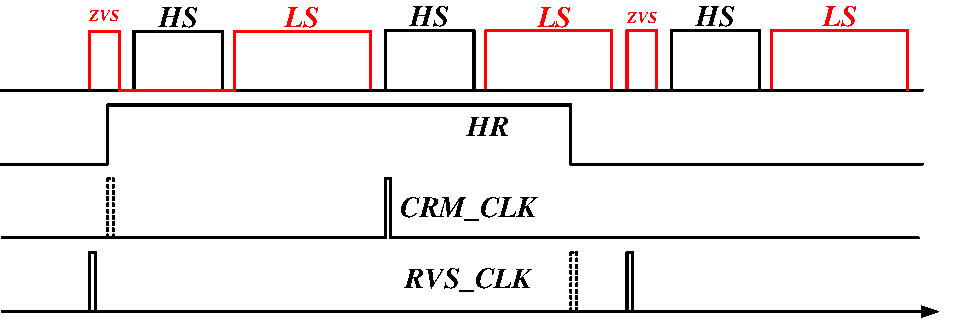
\includegraphics[width=0.8\linewidth]{figures/逻辑控制波形1.pdf}
    \caption{不同工作模式切换波形图}
    \label{fig:逻辑控制波形1}
\end{figure} 

同时为了防止初值出现系统模式切换不连贯甚至功率管同时开通导致电源短路的问题,引入了SR锁存器2和3来预防在一个开关周期未结束时即使信号HR逻辑电平发生变化也不立即切换模式的解决方案。具体电路过程的波形图如图~\ref{fig:逻辑控制电路原理图}所示,当HR从低电平变为高电平时,此时刻RVS模式的工作周期正处于低边功率管导通的软启动阶段,如果此刻立即切换为CRM模式导通高边功率管,很大可能造成同时导通问题。本逻辑控制电路中通过SR锁存器2和3产生了信号T\_CRM和T\_RVS,这两个信号代表了两种模式下整个开关周期的脉宽长度,即在周期结束之前,即使HR电平发生变化,也不允许出现切换模式的操作,防止误触发。

\subsection{逻辑控制电路仿真分析}

\begin{figure}[htbp] 
    \centering
    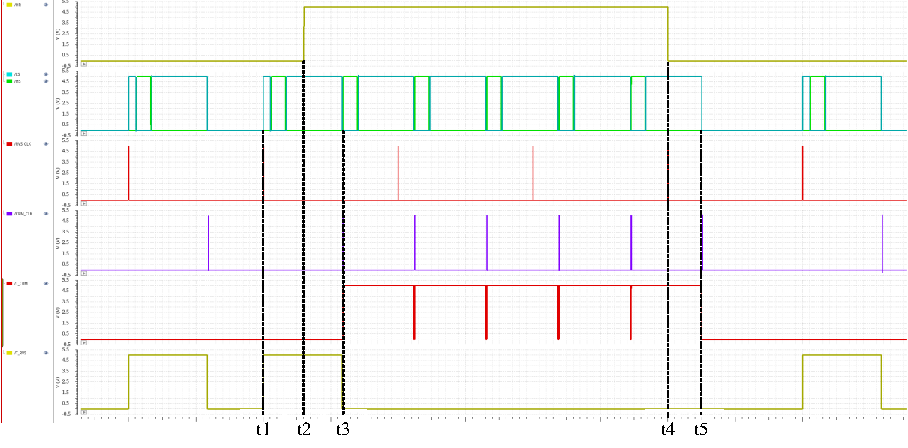
\includegraphics[width=0.8\linewidth]{figures/逻辑控制波形2.pdf}
    \caption{逻辑控制电路具体仿真波形图}
    \label{fig:逻辑控制波形2}
\end{figure} 

逻辑控制电路的具体仿真波形图如图~\ref{fig:逻辑控制波形2}所示,详细显示了在系统整体仿真时的工作模式,可以观察到在$V_{HB}$谷底信号附近t1时刻产生的控制信号RVS\_CLK,此时RVS模式开关周期信号T\_RVS同时变为高电平;当工作到t2时刻时,信号HR被拉高到高电平,但由于此时仍处于T\_RVS为高电平的状态下,因此并未立刻切换工作模式,而是在t3时刻RVS模式开关周期结束后接收到信号CRM\_CLK后开启CRM工作模式。当HR从高电平切换为低电平时同样并未立刻发生开关周期的立刻切换。此仿真波形很好的验证了该逻辑控制电路的设计,完成了其基本功能,符合系统需要。


%\section{保护电路}
%
%\subsection{过温保护}
%\subsection{过压保护}

\section{系统整体仿真}


\subsection{恒流模式仿真}

\begin{figure}[htbp] 
    \centering
    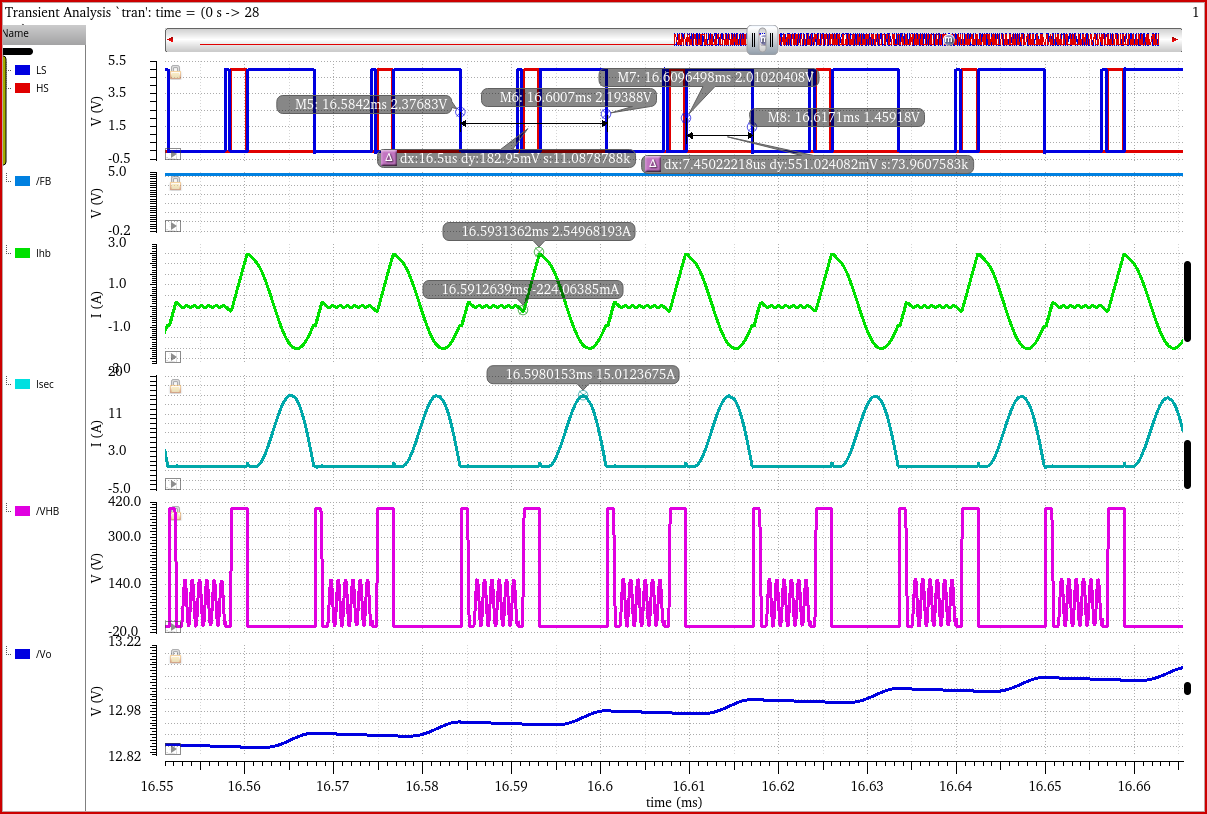
\includegraphics[width=0.8\linewidth]{figures/constant_current.png}
    \caption{恒流控制模式仿真波形图}
    \label{fig:恒流控制模式仿真波形图}
\end{figure} 

图~\ref{fig:恒流控制模式仿真波形图}为恒流控制模式的仿真波形图,电路的输入电压为直流输入370V,输出额定电压20V,负载电阻为5Ω,系统工作在重载工作情况下。此时输出电压未达到额定电压附近,副边反馈电压$V_{FB}$被上拉电阻保持在最高电位。根据式\eqref{eq:Io_1}可以算得输出电流为8.6A,同时将仿真波形内的副边电流通过Virtuoso软件内置计算器求平均得8.406A,和计算值相似,证明恒流模式设计正确。但由于此时工作在RVS模式下,开关周期16us,退磁时间7.5us,故实际输出电流为3.94A,符合变换器芯片设计要求,通过调整原边电感电流采样电阻即可调整恒流模式充电电流大小。

\subsection{恒压模式仿真}

\subsubsection{重载工况}


图~\ref{fig:重载工况仿真波形图}显示为恒压控制模式中满载情况下的电路仿真波形图。由仿真图可见,在重输出负载电流的情况下,电路工作在CRM模式,每个开关周期在原副边能量传递完成副边电流$I_{sec}$降为0A时结束本周期,并经过死区时间后开启下一个开关周期。通过在这种模式下交替通断高低边功率管将平均输出电压稳定在19.98V,输出平均电流为5A,副边反馈电压$V_{FB}$稳定在3.79V。

\begin{figure}[htbp] 
    \centering
    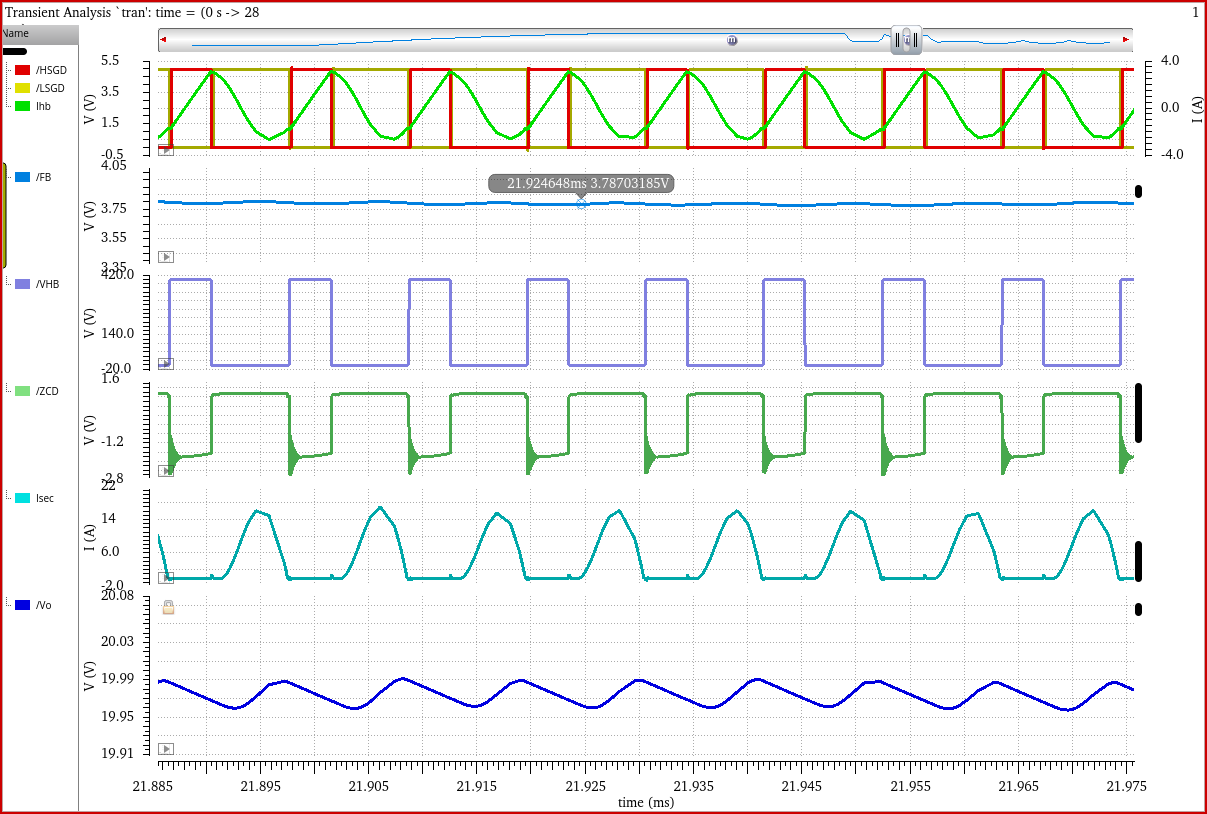
\includegraphics[width=0.8\linewidth]{figures/5A1_polt.png}
    \caption{满载电路仿真波形图}
    \label{fig:重载工况仿真波形图}
\end{figure} 

图~\ref{fig:重载工况单周期仿真波形图}是图~\ref{fig:重载工况仿真波形图}单个周期内电路仿真波形图,通过对单个开关周期的放大可以观察到,电路完成了在退磁完成时刻关闭低边功率管的功能,且半桥节点电压$V_{HB}$在死区时间内在负向原边电感电流的充能下被抬升至输入电压大小,实现CRM模式下的功率管软开关技术,当高边功率管零电压导通时,电感电流采样电阻电压$V_{cs}$并未出现电压尖峰,电路性能良好。

\begin{figure}[htbp] 
    \centering
    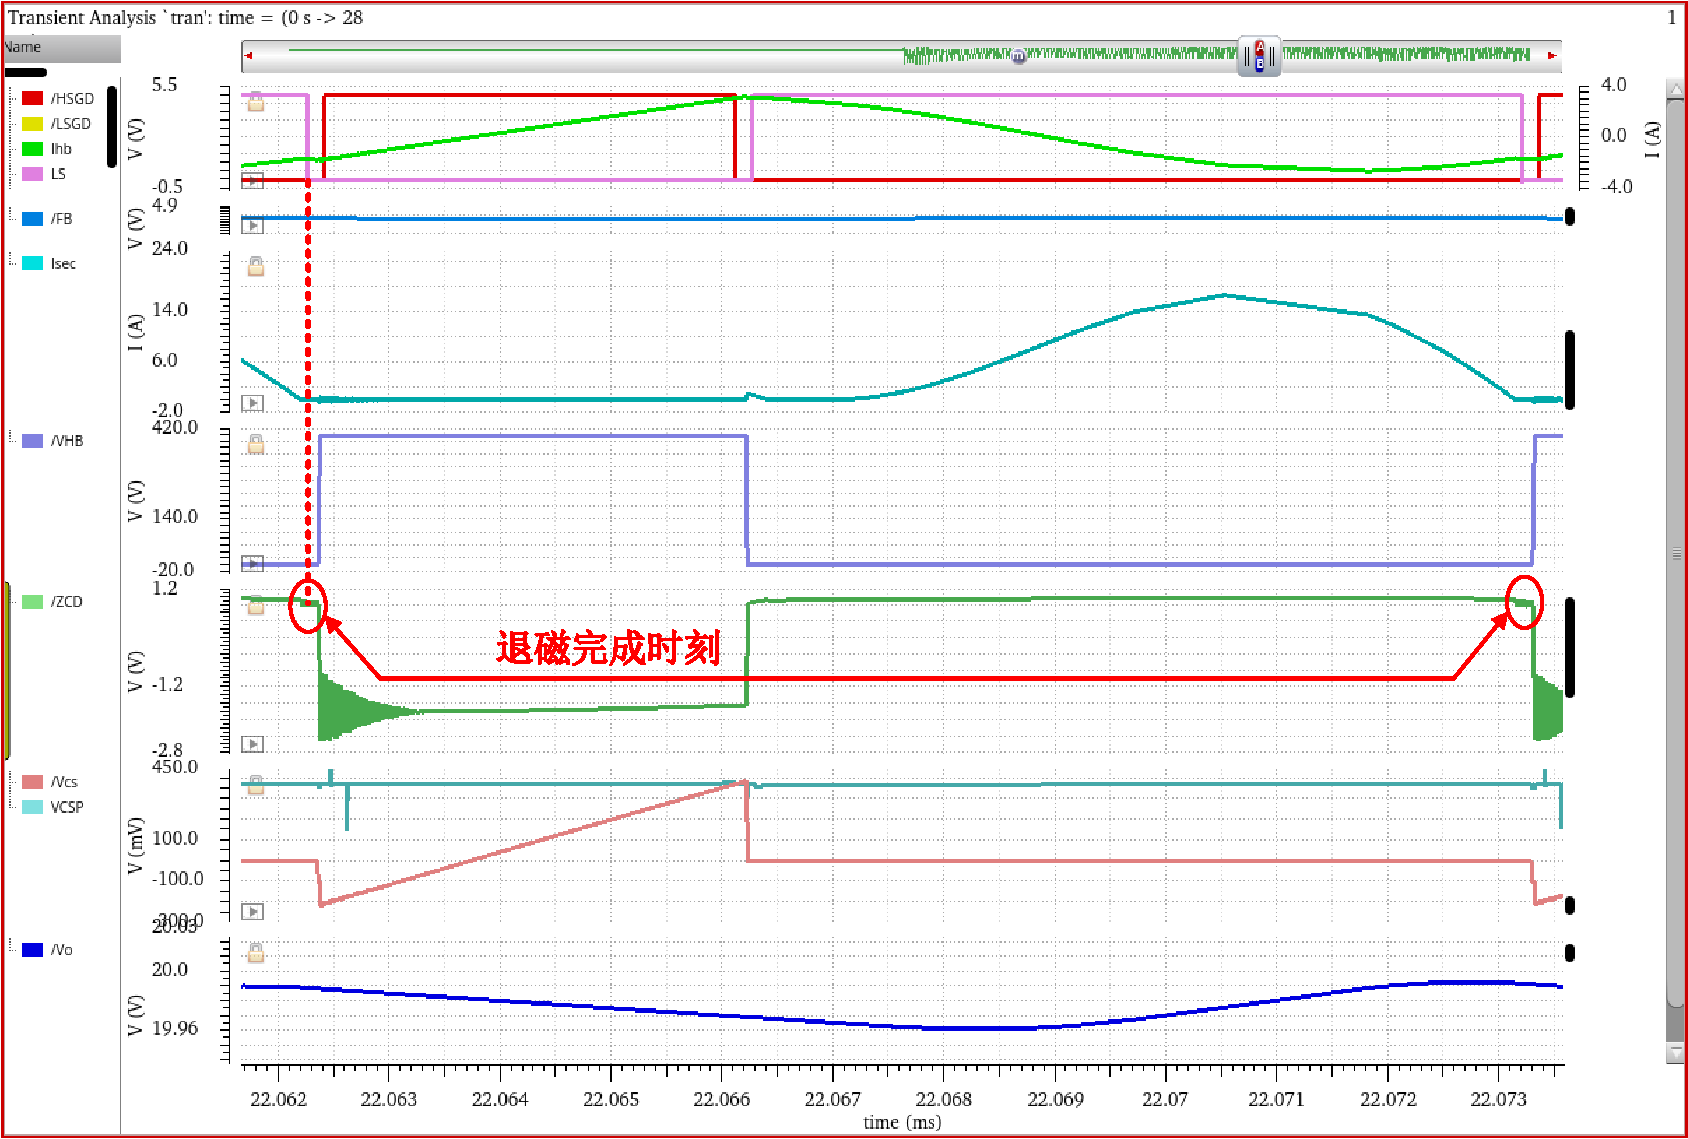
\includegraphics[width=0.8\linewidth]{figures/满载仿真图2.pdf}
    \caption{满载电路单周期仿真波形图}
    \label{fig:重载工况单周期仿真波形图}
\end{figure} 

\subsubsection{轻载工况}

%\subsubsection{空载工况}
%在次级侧调节(SSR)反激式转换器中,由于输出是通过光耦合器采样的,零载时的频率可以通过突发模式(跳过一些周期)来降低。当负载从零变为重载时,光耦合器会及时将负载信息传输到 IC 控制器,以便快速退出突发模式并提高动态响应速度。对于初级侧调节(PSR)转换器,输出状态不能及时反馈给控制器,而是每个周期采样一次,所以 PSR 转换器没有突发模式。

\subsubsection{负载跳变}

图~\ref{fig:负载2.5_5A跳变仿真波形图}是非对称半桥反激式变换器恒压控制模式下的输出负载电流从2.5A跳变到5A的仿真波形图。可以观察到在2.5A的负载电流下,电路工作在RVS工作模式下,此时副边反馈电压$V_{FB}$等于1.73V,位于谷值锁定稳定区域,谐振谷值被锁定在第二个谷底处。当负载发生跳变后,$V_{FB}$迅速增大超过$V_{FBRVS2CRM}$,电路切换为CRM模式,输出电压下冲变化量约为317mV,经过0.5ms后输出电压恢复稳定,电路响应速度良好。


\begin{figure}[htbp] 
    \centering
    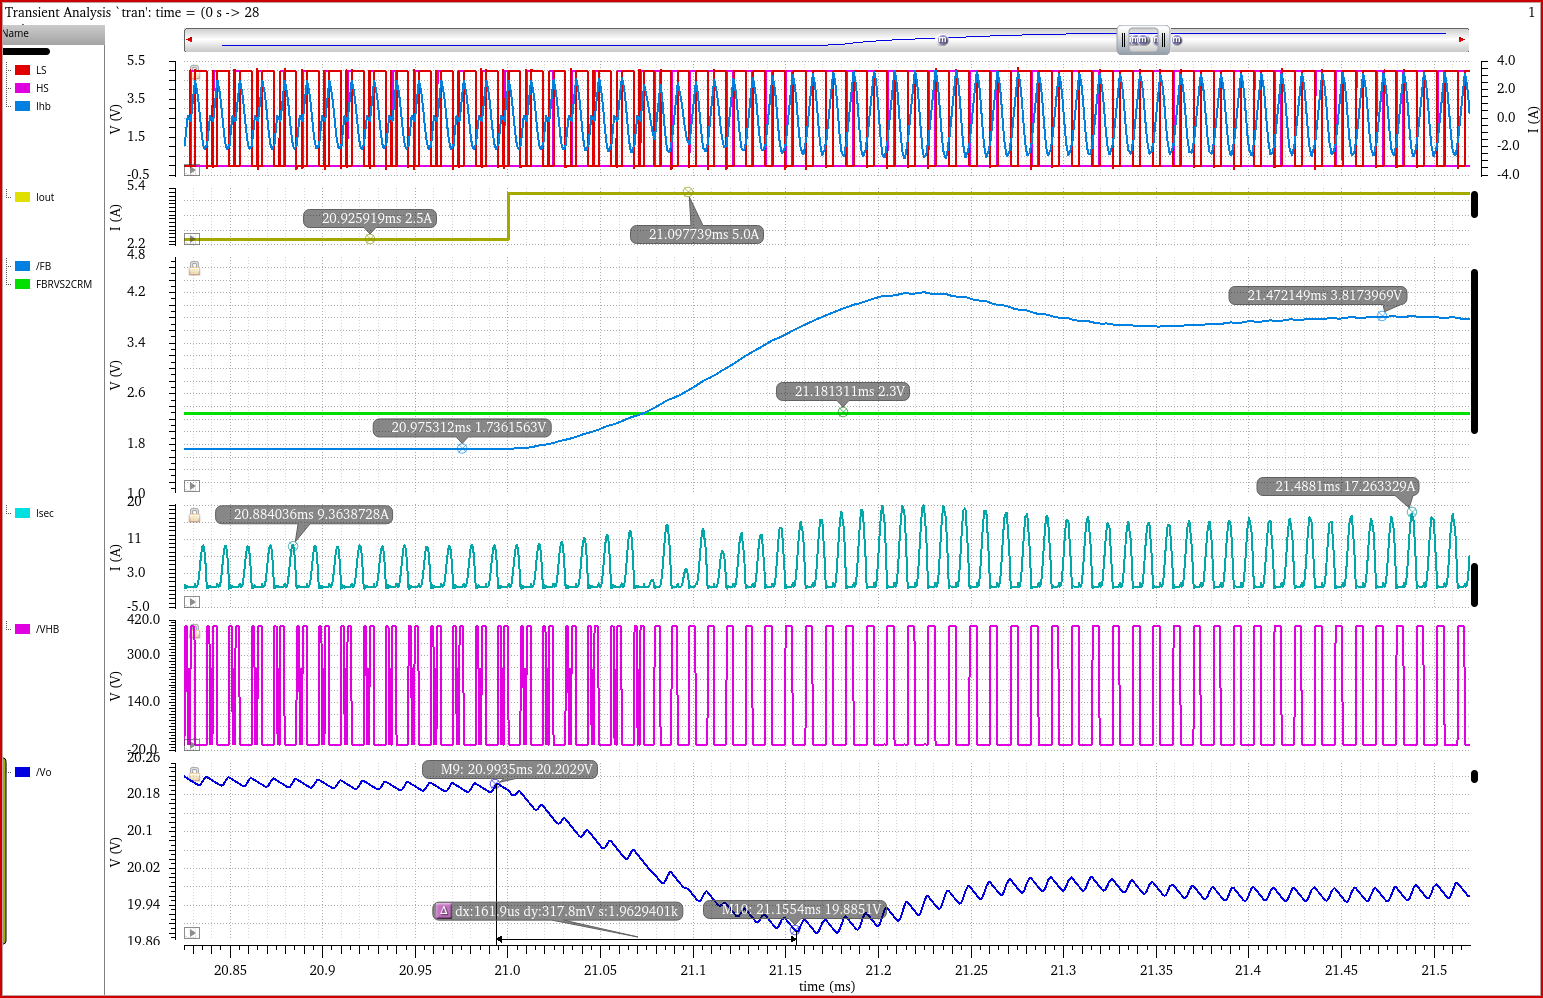
\includegraphics[width=0.8\linewidth]{figures/2.5A_ 5A.png}
    \caption{负载2.5-5A跳变仿真波形图}
    \label{fig:负载2.5_5A跳变仿真波形图}
\end{figure} 



• 满载下输出电压纹波仿真
• 恒压下20V\_5A、20V\_3A、20V\_1A、5V\_5A、5V\_3A、5V\_1A的仿真图

• 恒压下极轻载的仿真测试BM模式

• 恒压下负载跳变的仿真



\section{小结}




